\chapter{Experimental Results}
\label{chap:experiment}
In this chapter we introduce the evaluation metrics and dataset adopted in our work firstly. Then the experiment results are shown and analyzed in detail. We also compare our model with other advanced works.

\section{Dataset}

In visual relationship detection / scene graph generation, most of related works adopt Visual Genome~\cite{krishna2017visual} as dataset. Compared with another dataset VRD, the scenes of Visual Genome are more diverse and challengeable. It contains 108,077 Images with 2.3 million relationships.

However, the original Visual Genome has the problems such as overlapping bounding boxes and ambiguous object and predicate names. We adopt the Visual Genome cleaned up by Danfei et al.~\cite{xu2017scene}  and also use the most frequency 150 object categories and 50 predicates for the experiments on our deep learning model. In this thesis, we use $ 62,723 $ images as the train dataset, and $ 26,446 $ images as the test dataset.

\begin{figure}[!hbtp]
	\centering
	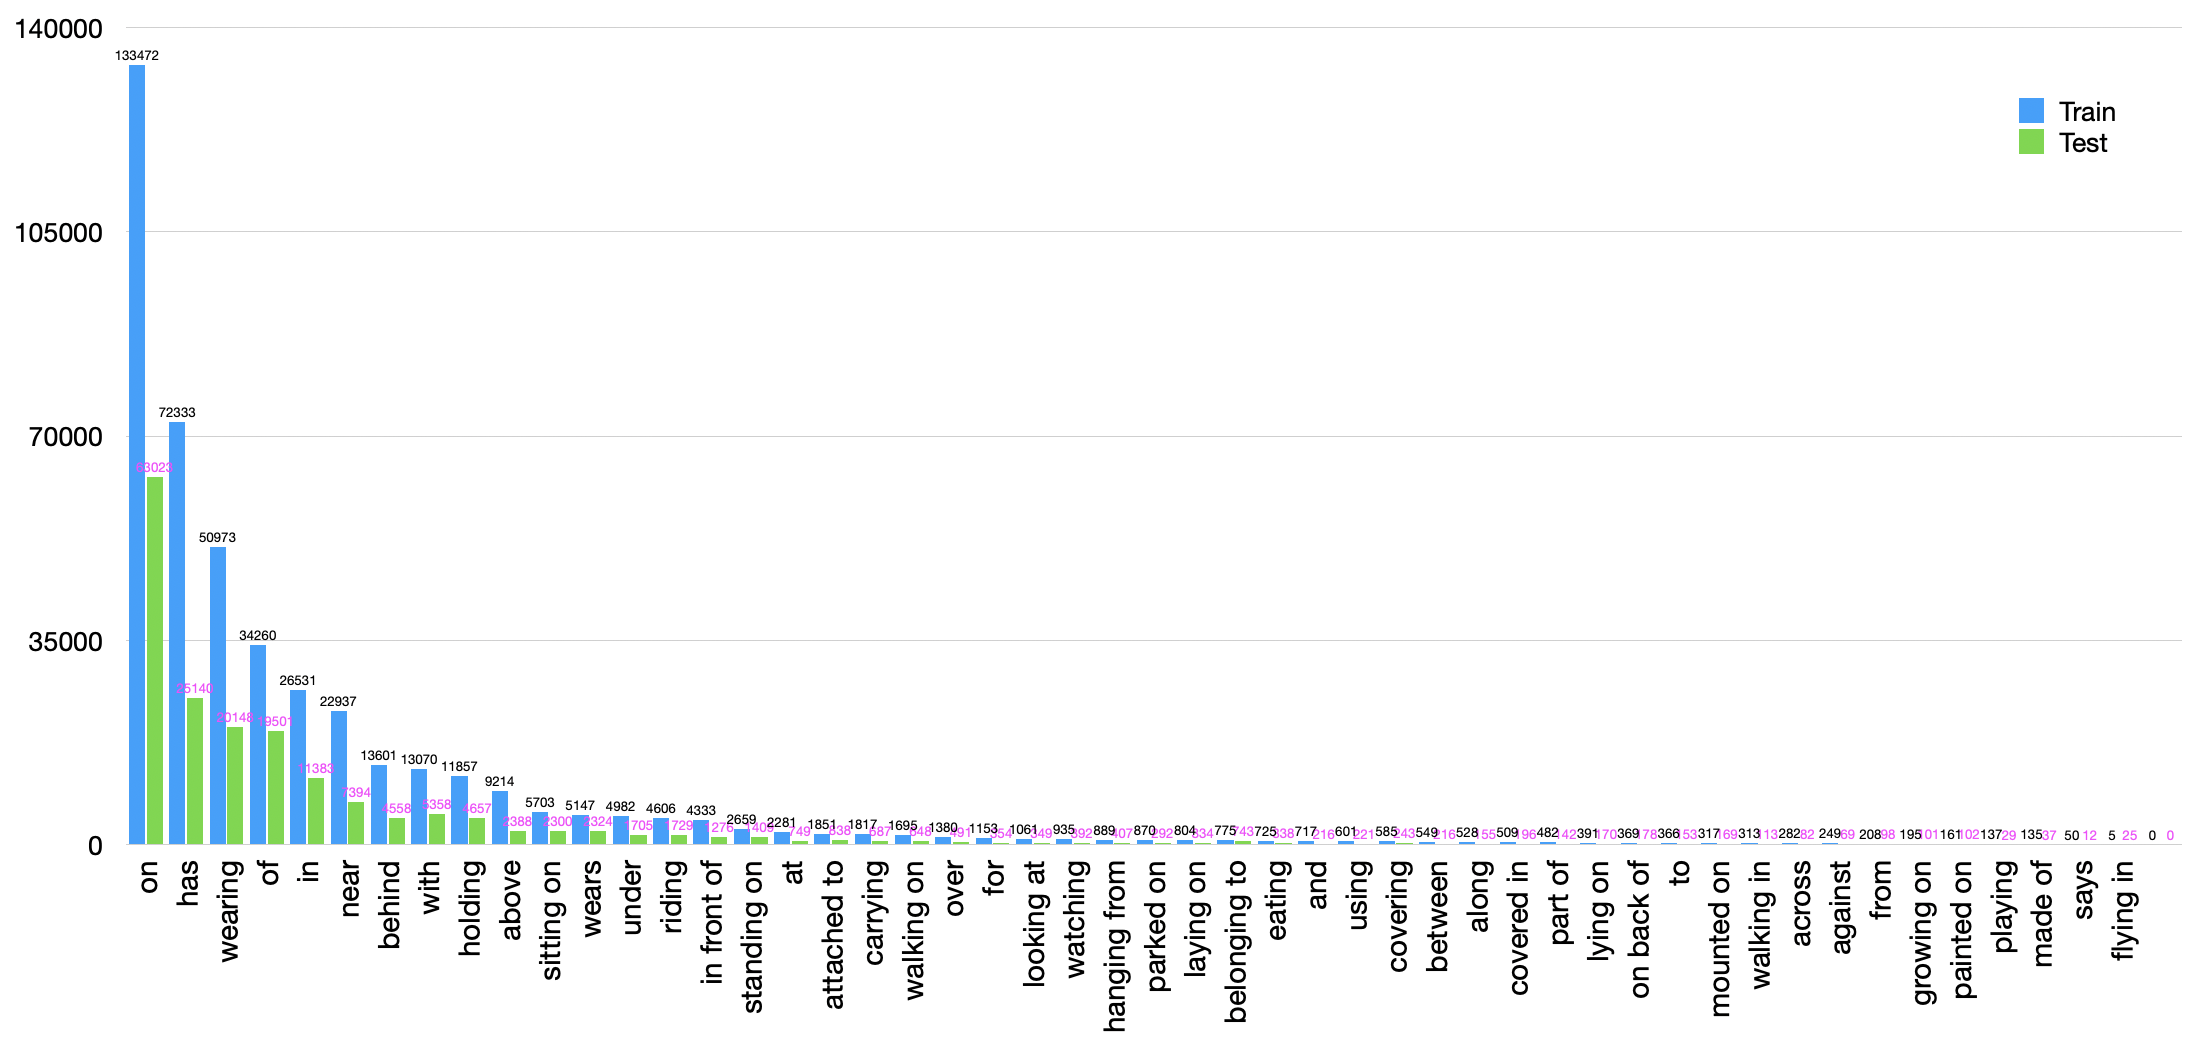
\includegraphics[width=0.9\linewidth]{figures/predicates}
	\caption[Predicate distribution of VG dataset]{Predicate distribution of VG dataset.}
	\label{fig:predicates}
\end{figure}

Figure~\ref{fig:predicates} is the predicate distribution in the data set we selected. We can conclude that the train data set and the test data set have the same predicate distribution.

\section{Evaluation Metrics}


Visual relationship detection involves object classification, localization and predicate prediction. As we mentioned before, the vrd problem has three tasks, and each task has different input information:

\begin{enumerate}[\qquad  $\bullet$]
\item Predicate Classification(\textbf{predcls}): The input is an image and a set of objects with their object classes and bounding boxes. The classes and locations of the objects are known. The model predicts the matching of subject-object pairs and their predicates.

\item Scene Graph Classification(\textbf{sgcls}): The input is an image and a set of objects with their boun- ding boxes. The classes of the objects are unknown. The model classifies the objects and predicts the matching of subject-object pairs and their predicates.

\item Scene Graph Detection(\textbf{sgdet}): The input is an image. The output involves the classes of the subjects and objects, the predicates of each subject-object pairs and the bounding boxes of each subject and object which have at least 0.5 overlap with the bounding boxes in ground truth.
\end{enumerate}

In our experiment, due to the incomplete annotation of the true relationship, we use the relationship detection $ Recall@K $ as an evaluation indicator, which measures the scores of the true relationship triples in the top K most reliable triple predictions that appear in the image.


\section{Experiments on Pixel-based Attention}
In Section~\ref{sec:pixel_base}, we put forward related ideas, through the attention map in Figure~\ref{fig:method1baseline} to find possible relationships in the detected pictures. We hope that the most relevant area can be directly reflected in the attention map, so we designed an Attention loss function(see Eq.~\ref{pixel_attention_loss}) so that the attention weights of the relevant area are higher than the non-relevant area.

We tried to add a Multihead Self-Attention module after obtaining the image feature in VGG16 based on the code of RelDN~\cite{zhang2019graphical},  so that we obtained a new image feature with a size of $ [bs, 512, 50, 66]  $and an  Attention map with a size of $ [bs, 3300, 3300] $, where bs is batch size=2. We build the baseline as the Fig.~\ref{fig:method1baseline} shown.

\subsubsection{Result of the Pixel Attention Loss  Function}
Figure~\ref{fig:motor_attention} shows the result of our training. Figure~\ref{fig:motor_img} is our input, and Figure~\ref{fig:motor_attention_map} is the corresponding attention map. In order to show it well, we normalized it and drew it through Matlab.

From the results, our attention loss has made certain modifications to the attention map. But in general, the values in the attention map are relatively average, and there is no strong distinguish ability. For instance, the ground truth pair $ <man, motorcycle>  $ shown in Fig.~\ref{fig:motor_man0}, its location of the corresponding area in attention map shown in Fig.~\ref{fig:motor_map0}. We can see the attention values in the area of the attention map(Fig.~\ref{fig:motor_attention_map}) is not higher than other areas, even be low.

In general, we use our  average of attention weights  of each pair to replace the original pair score ($ score_{pair}=score_{subject }*score_{predicate}* score_{object} $) in the evaluation to sort relation pairs, and it does not improve the recall rate of the relation.

\begin{figure}[!h]
	\centering
	\subfigure[Image input.]{
		\begin{minipage}[t]{7.5cm}
			\centering
			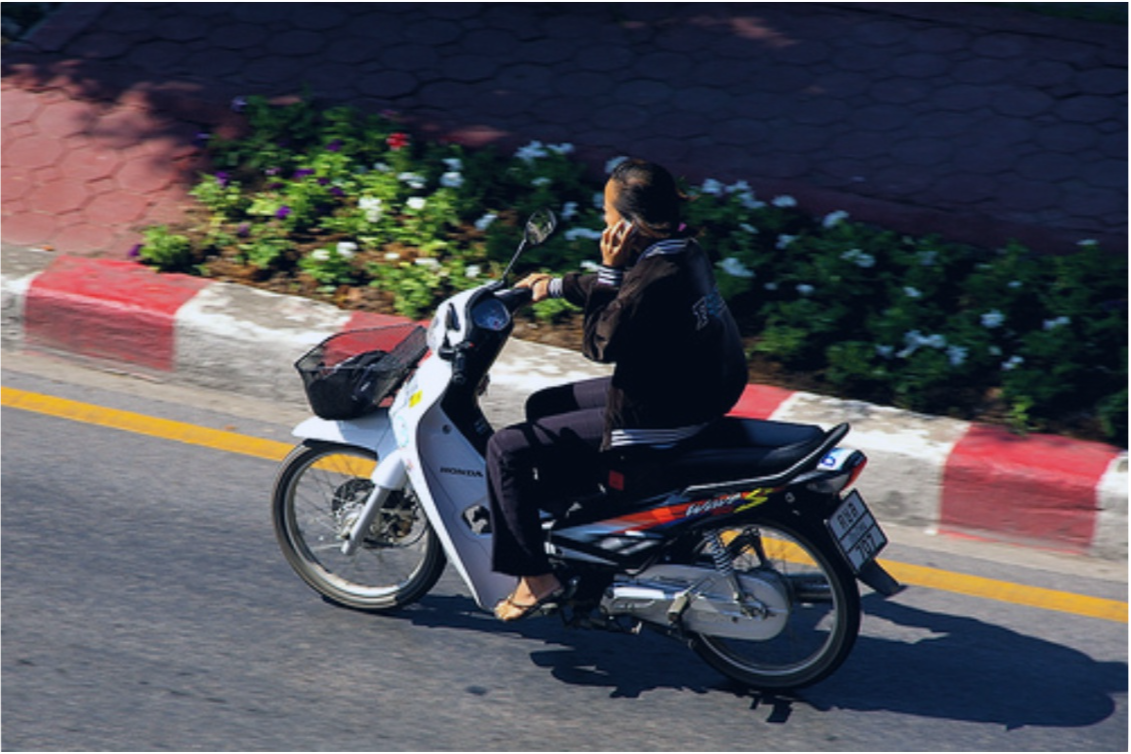
\includegraphics[width=0.95\linewidth]{figures/motor/img}
			\label{fig:motor_img}
	\end{minipage}}
	\subfigure[The result of a normalized Attention Map.]{
		\begin{minipage}[t]{7.5cm}
			\centering
			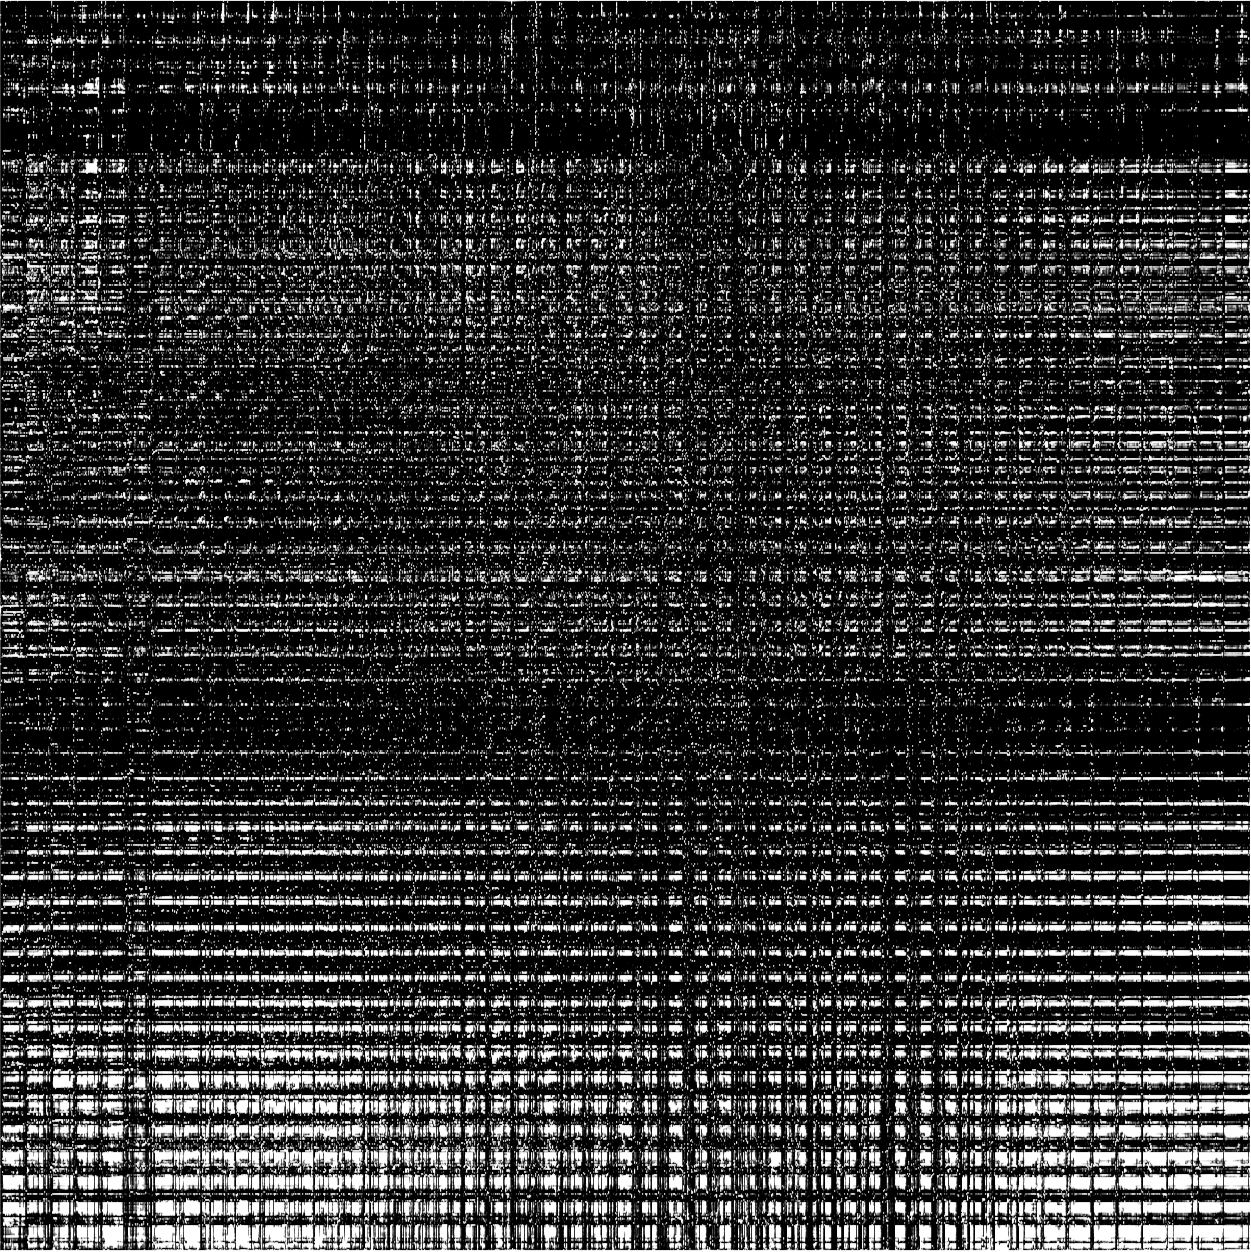
\includegraphics[width=0.95\linewidth]{figures/motor/attention}
			\label{fig:motor_attention_map}
	\end{minipage}}
	
	\caption[The result of a normalized Attention Map drawn by matlab]{The result of a normalized Attention Map drawn by matlab.}
	\label{fig:motor_attention}
\end{figure}


\subsubsection{Result analysis}

Then we analyzed the results, and we drew the position of all $ Att_{rel} $s and all $ Att_{no\_rel} $s in the attention map of image~\ref{fig:motor_img} , see Fig.~\ref{fig:overlap} $ (a) $ and $ (b) $ in the figure. And the overlap between them is shown in Figure $ (c). $ We found that $ Att_{rel }$ and $ Att_{no\_rel} $ have a very serious overlap, and are basically the same as $ Att_{rel }$, that is,  $ Att_{no\_rel} $ contains $ Att_{rel }$. The purpose of our Attention Loss is to make $ Att_{rel }$ higher and $ Att_{no\_rel }$ lower. The existence of this overlap makes its purpose very contradictory. For example, the area in Figure~\ref{fig:motor_all0} belongs to $ Att_{rel }$ but it also belongs to $ Att_{no\_rel }$ in Figure~\ref{fig:motor_all1}. We cannot make it higher and lower. This overlap in the image is shown in Figure~\ref{fig:motor_pair}. For example, for the same subject $ man $, there are  pairs $<man,ride,motorcycle>$, $ <man, \varnothing, wheel_1> $  and  $ <man, \varnothing, wheel_2>  $, their objects have an overlap, and the bounding box  of $ motor $ obviously contains the bounding box of  $ wheel $.

This overlap is not a special case. We found that almost all images have this situation, so the attention loss we designed is meaningless, and the idea of Piexl-based Attention also failed. We cannot use the attention between pixels to obtain which pair is most likely to have a relationship.

\begin{figure}[h!]
	\centering
	\subfigure[$<man,ride,motorcycle>$]{
		\begin{minipage}[t]{5cm}
			\centering
			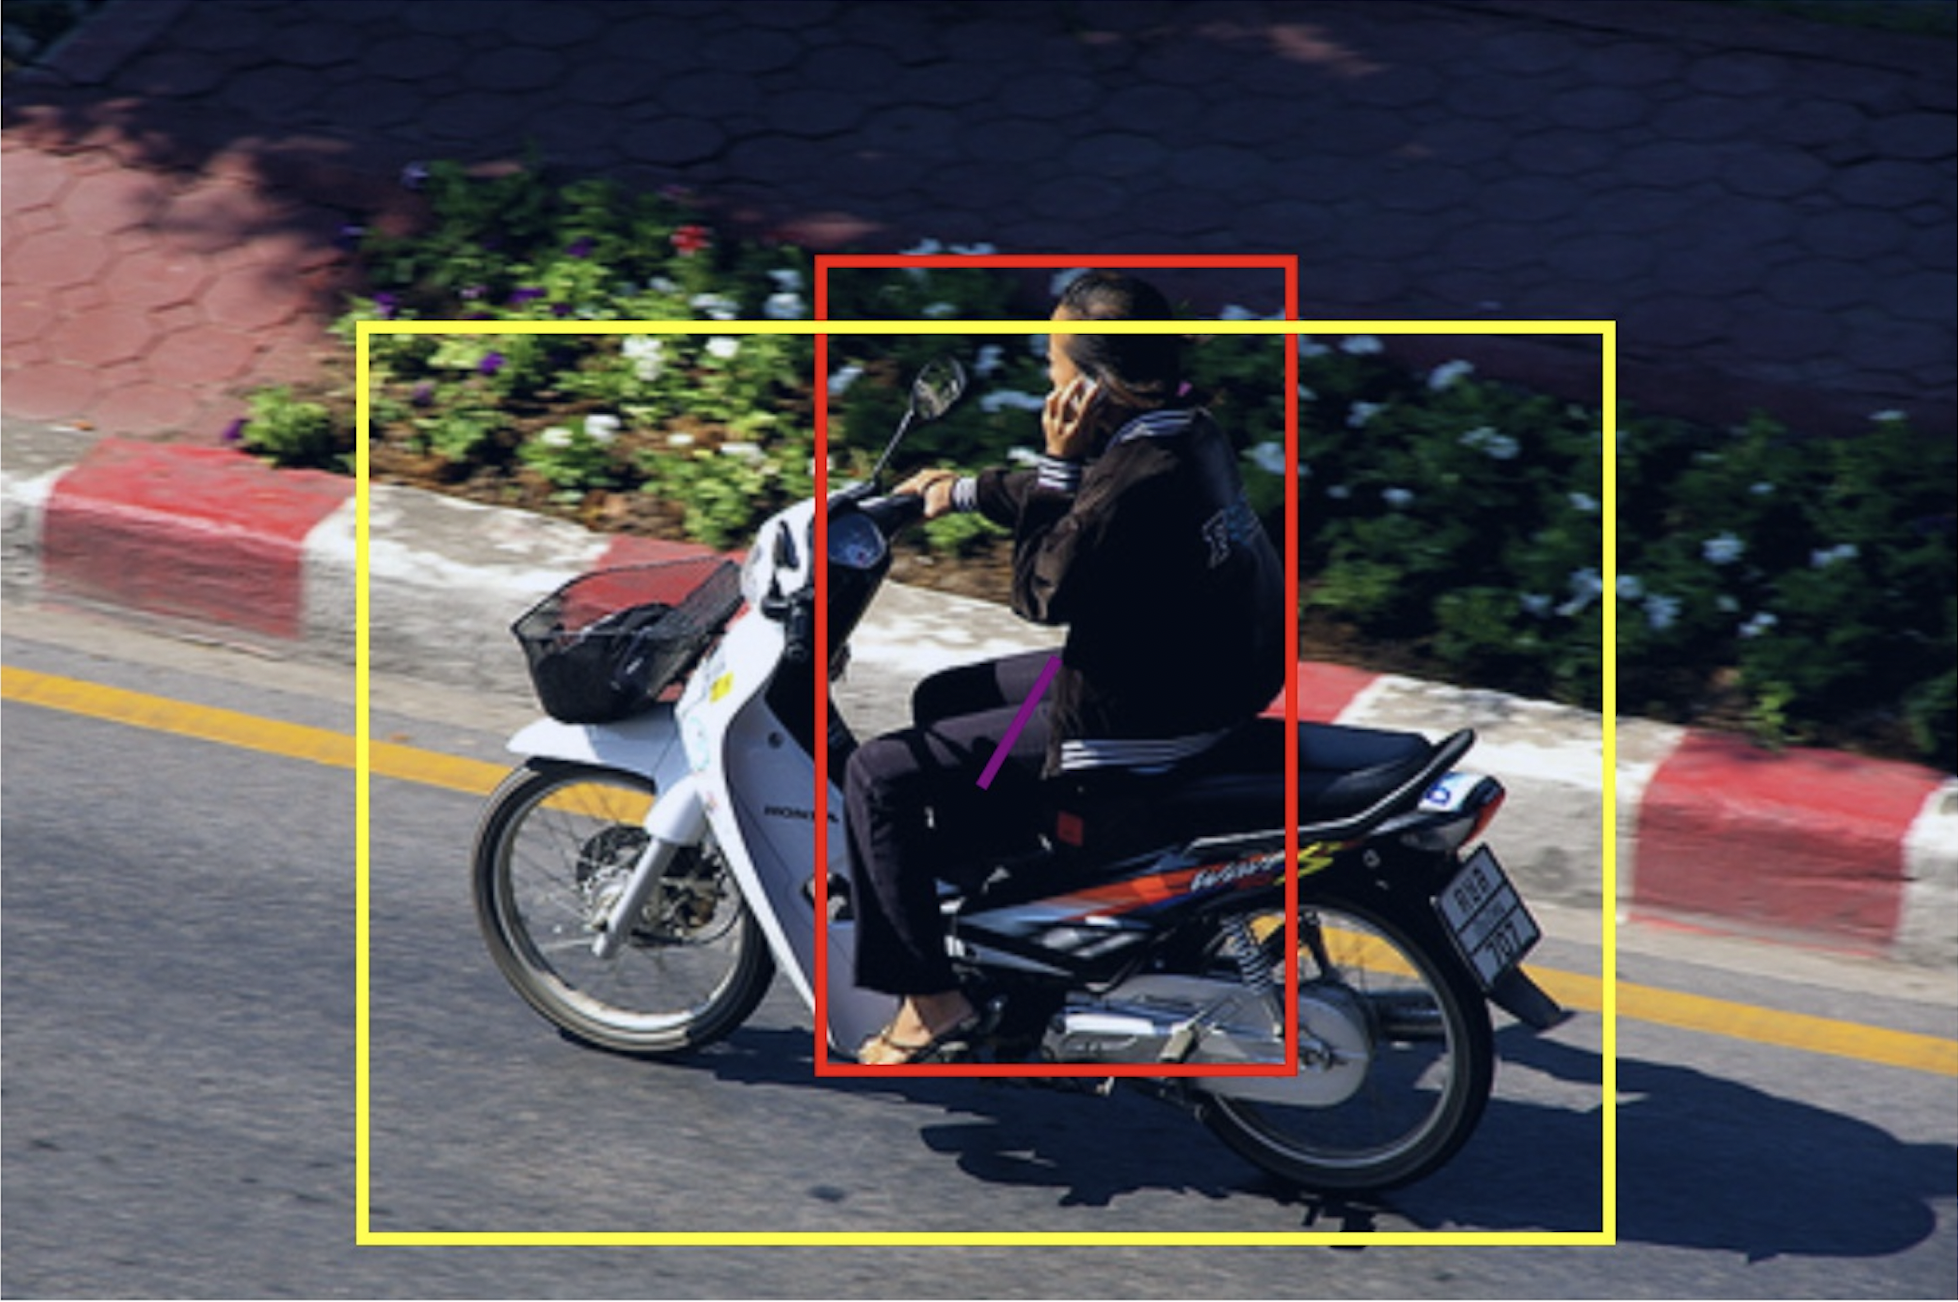
\includegraphics[width=0.9\linewidth]{figures/motor/man0}
			\label{fig:motor_man0}
	\end{minipage}}
	\subfigure[$ <man, \varnothing, wheel_1> $]{
		\begin{minipage}[t]{5cm}
			\centering
			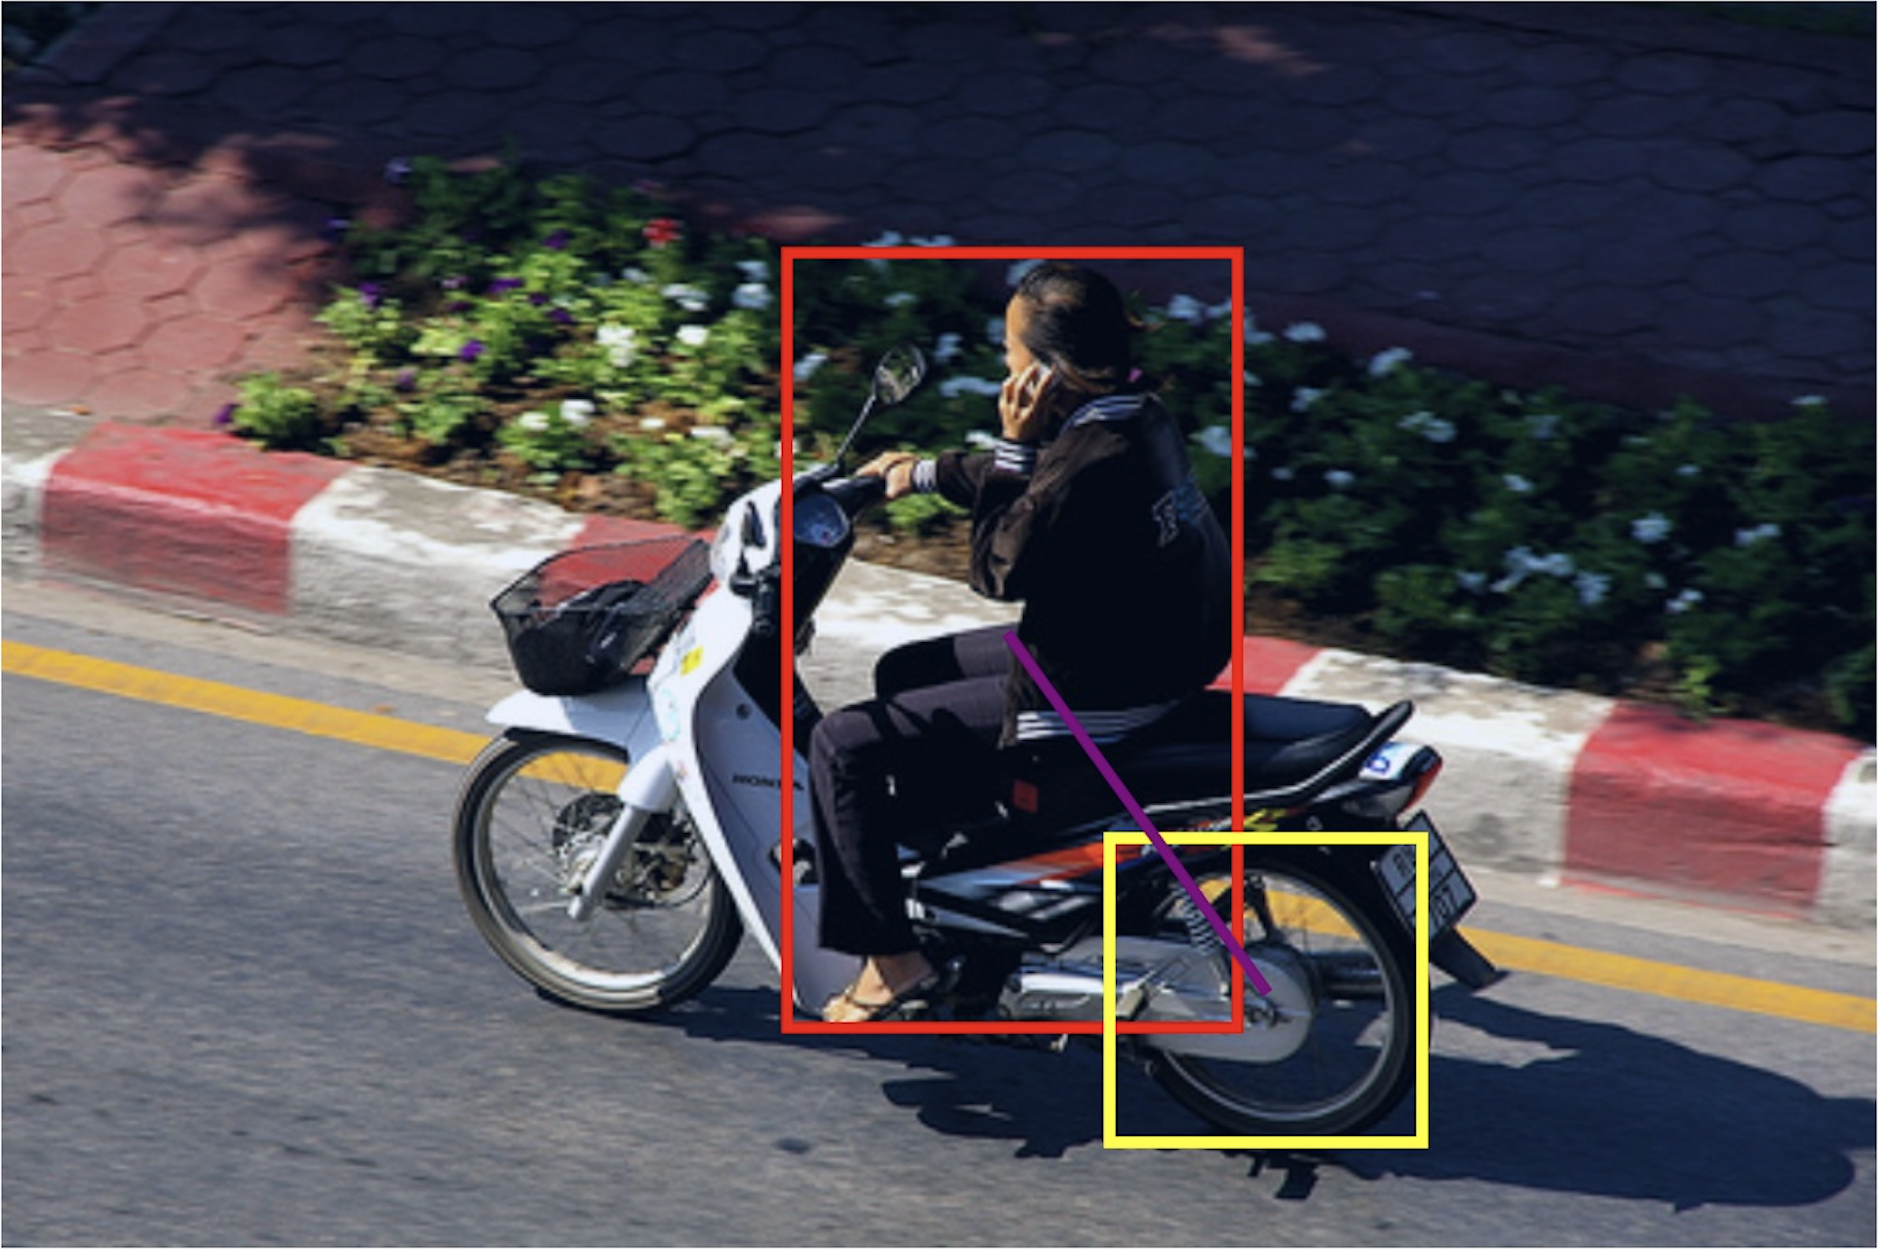
\includegraphics[width=0.9\linewidth]{figures/motor/man1}
			\label{fig:motor_map0}
	\end{minipage}}
	\subfigure[$ <man, \varnothing, wheel_2>  $]{
		\begin{minipage}[t]{5cm}
			\centering
			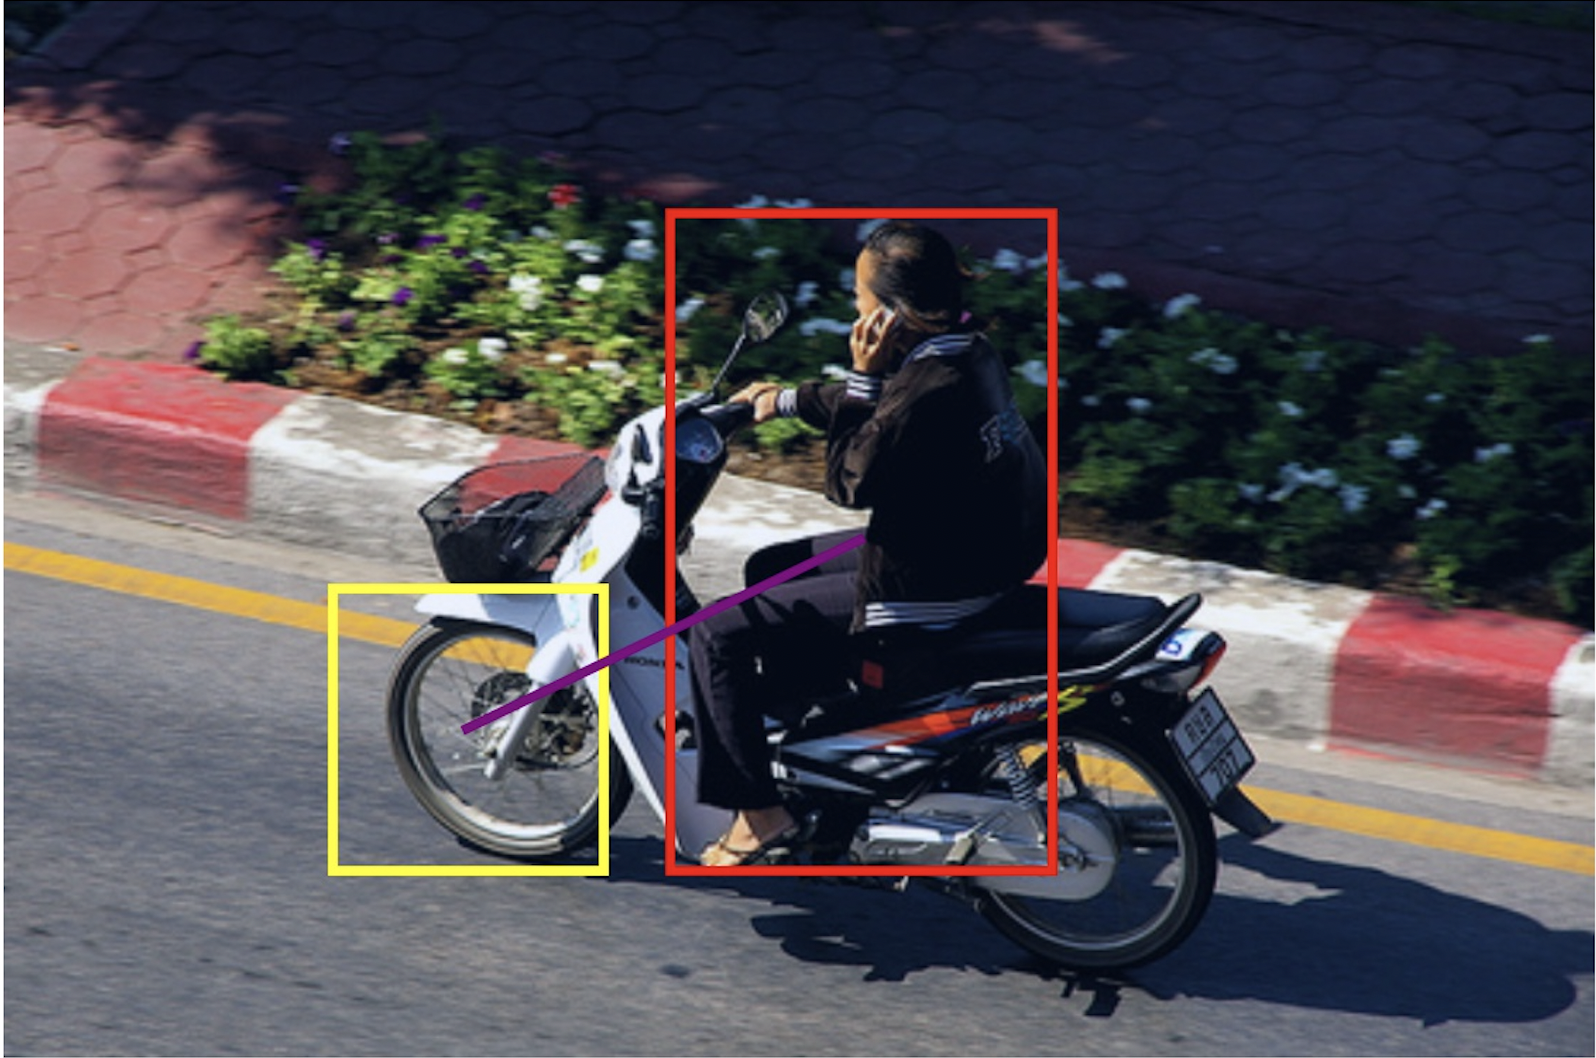
\includegraphics[width=0.9\linewidth]{figures/motor/man2}
			\label{fig:motor_man1}
	\end{minipage}}

	\subfigure[$Attention_{man \to motorcycle} $]{
		\begin{minipage}[t]{5cm}
			\centering
			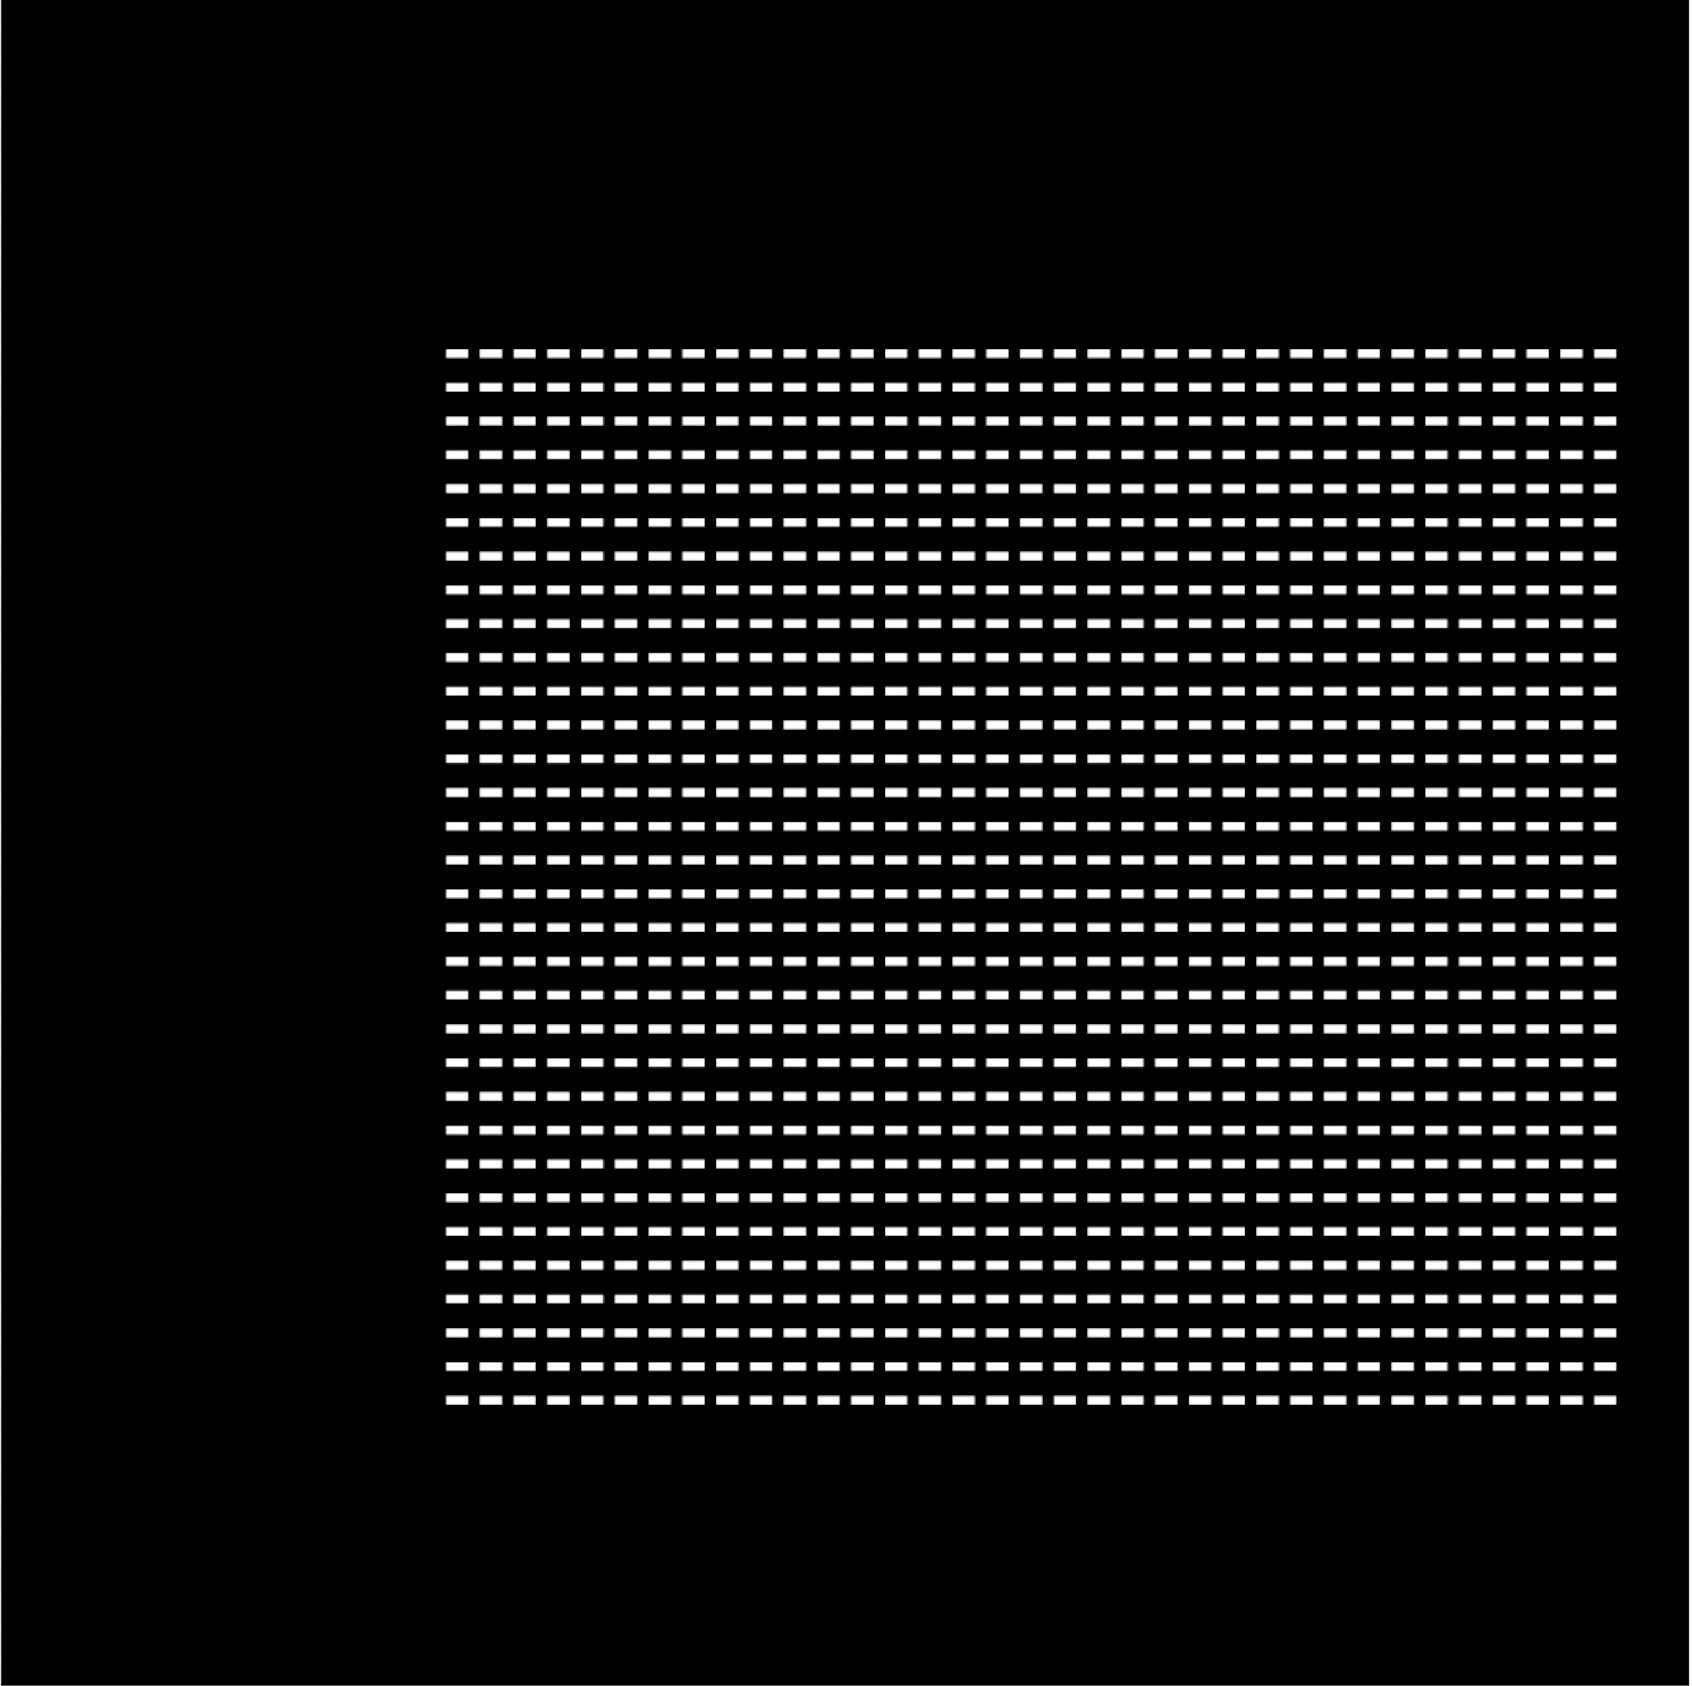
\includegraphics[width=0.9\linewidth]{figures/motor/map0}
			\label{fig:motor_map1}
	\end{minipage}}
	\subfigure[$Attention_{man \to wheel_1} $]{
		\begin{minipage}[t]{5cm}
			\centering
			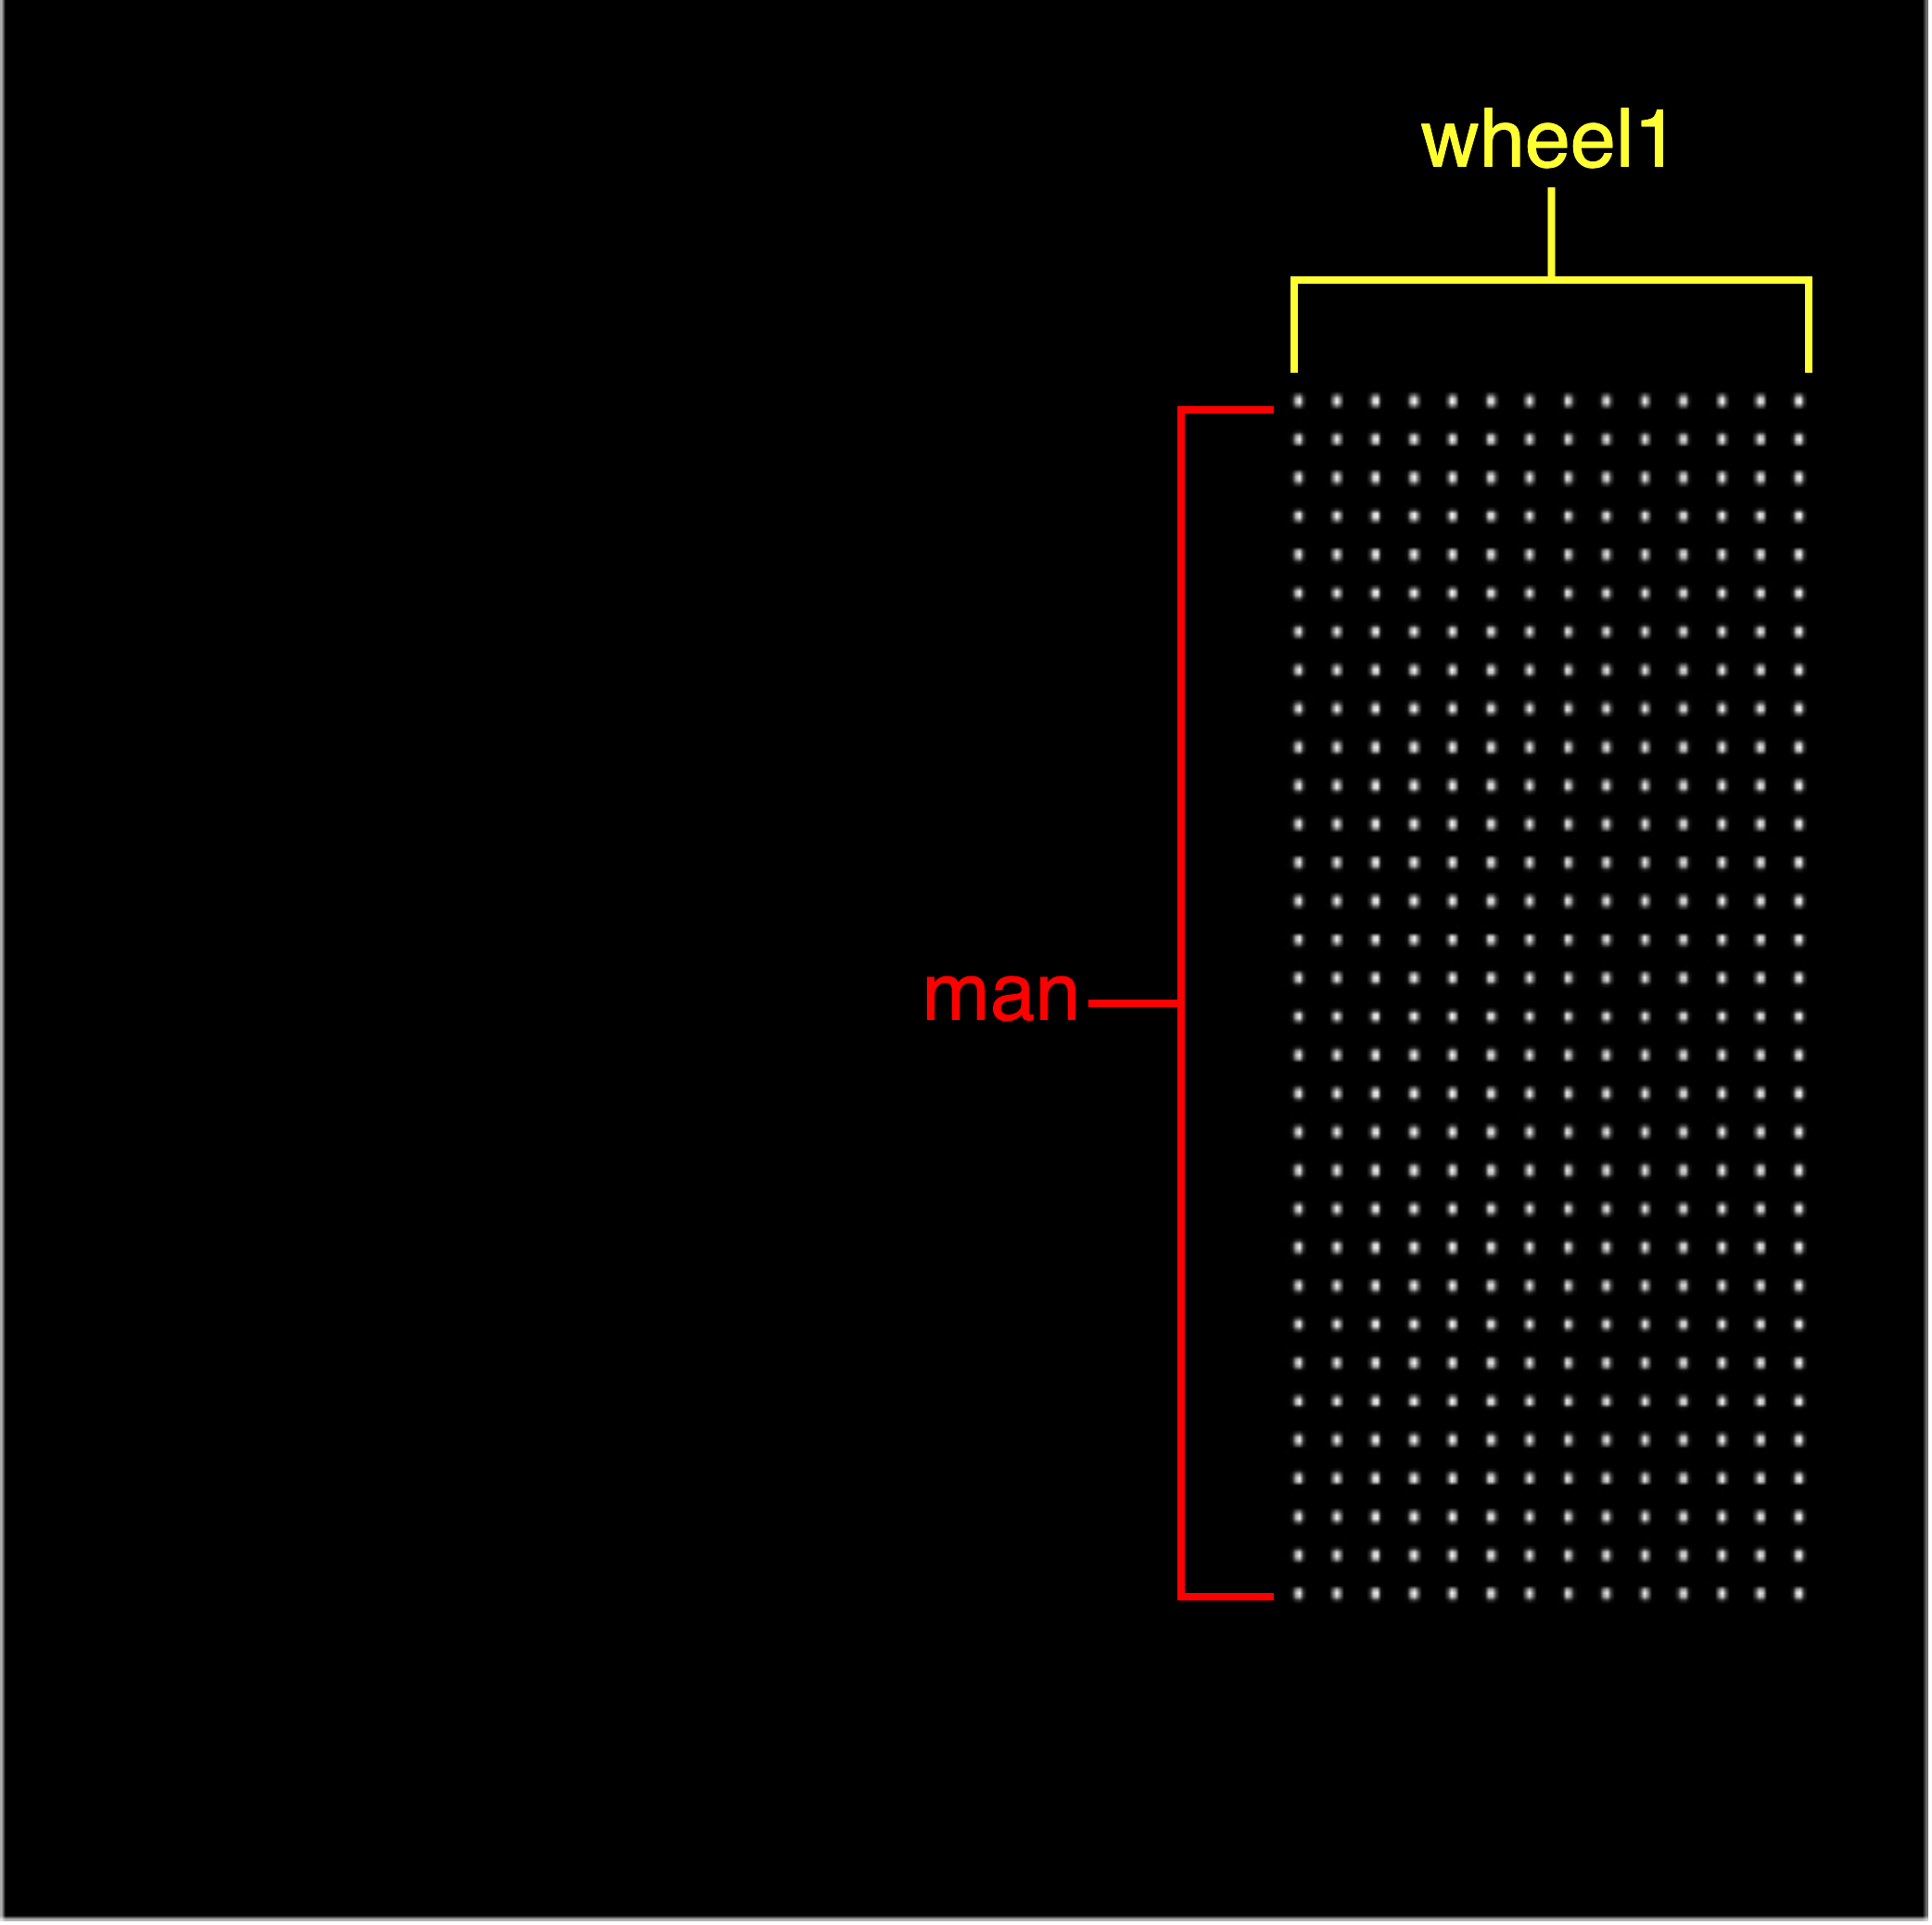
\includegraphics[width=0.9\linewidth]{figures/motor/map1}
			\label{fig:motor_man2}
	\end{minipage}}
	\subfigure[$Attention_{man \to wheel_2} $]{
		\begin{minipage}[t]{5cm}
			\centering
			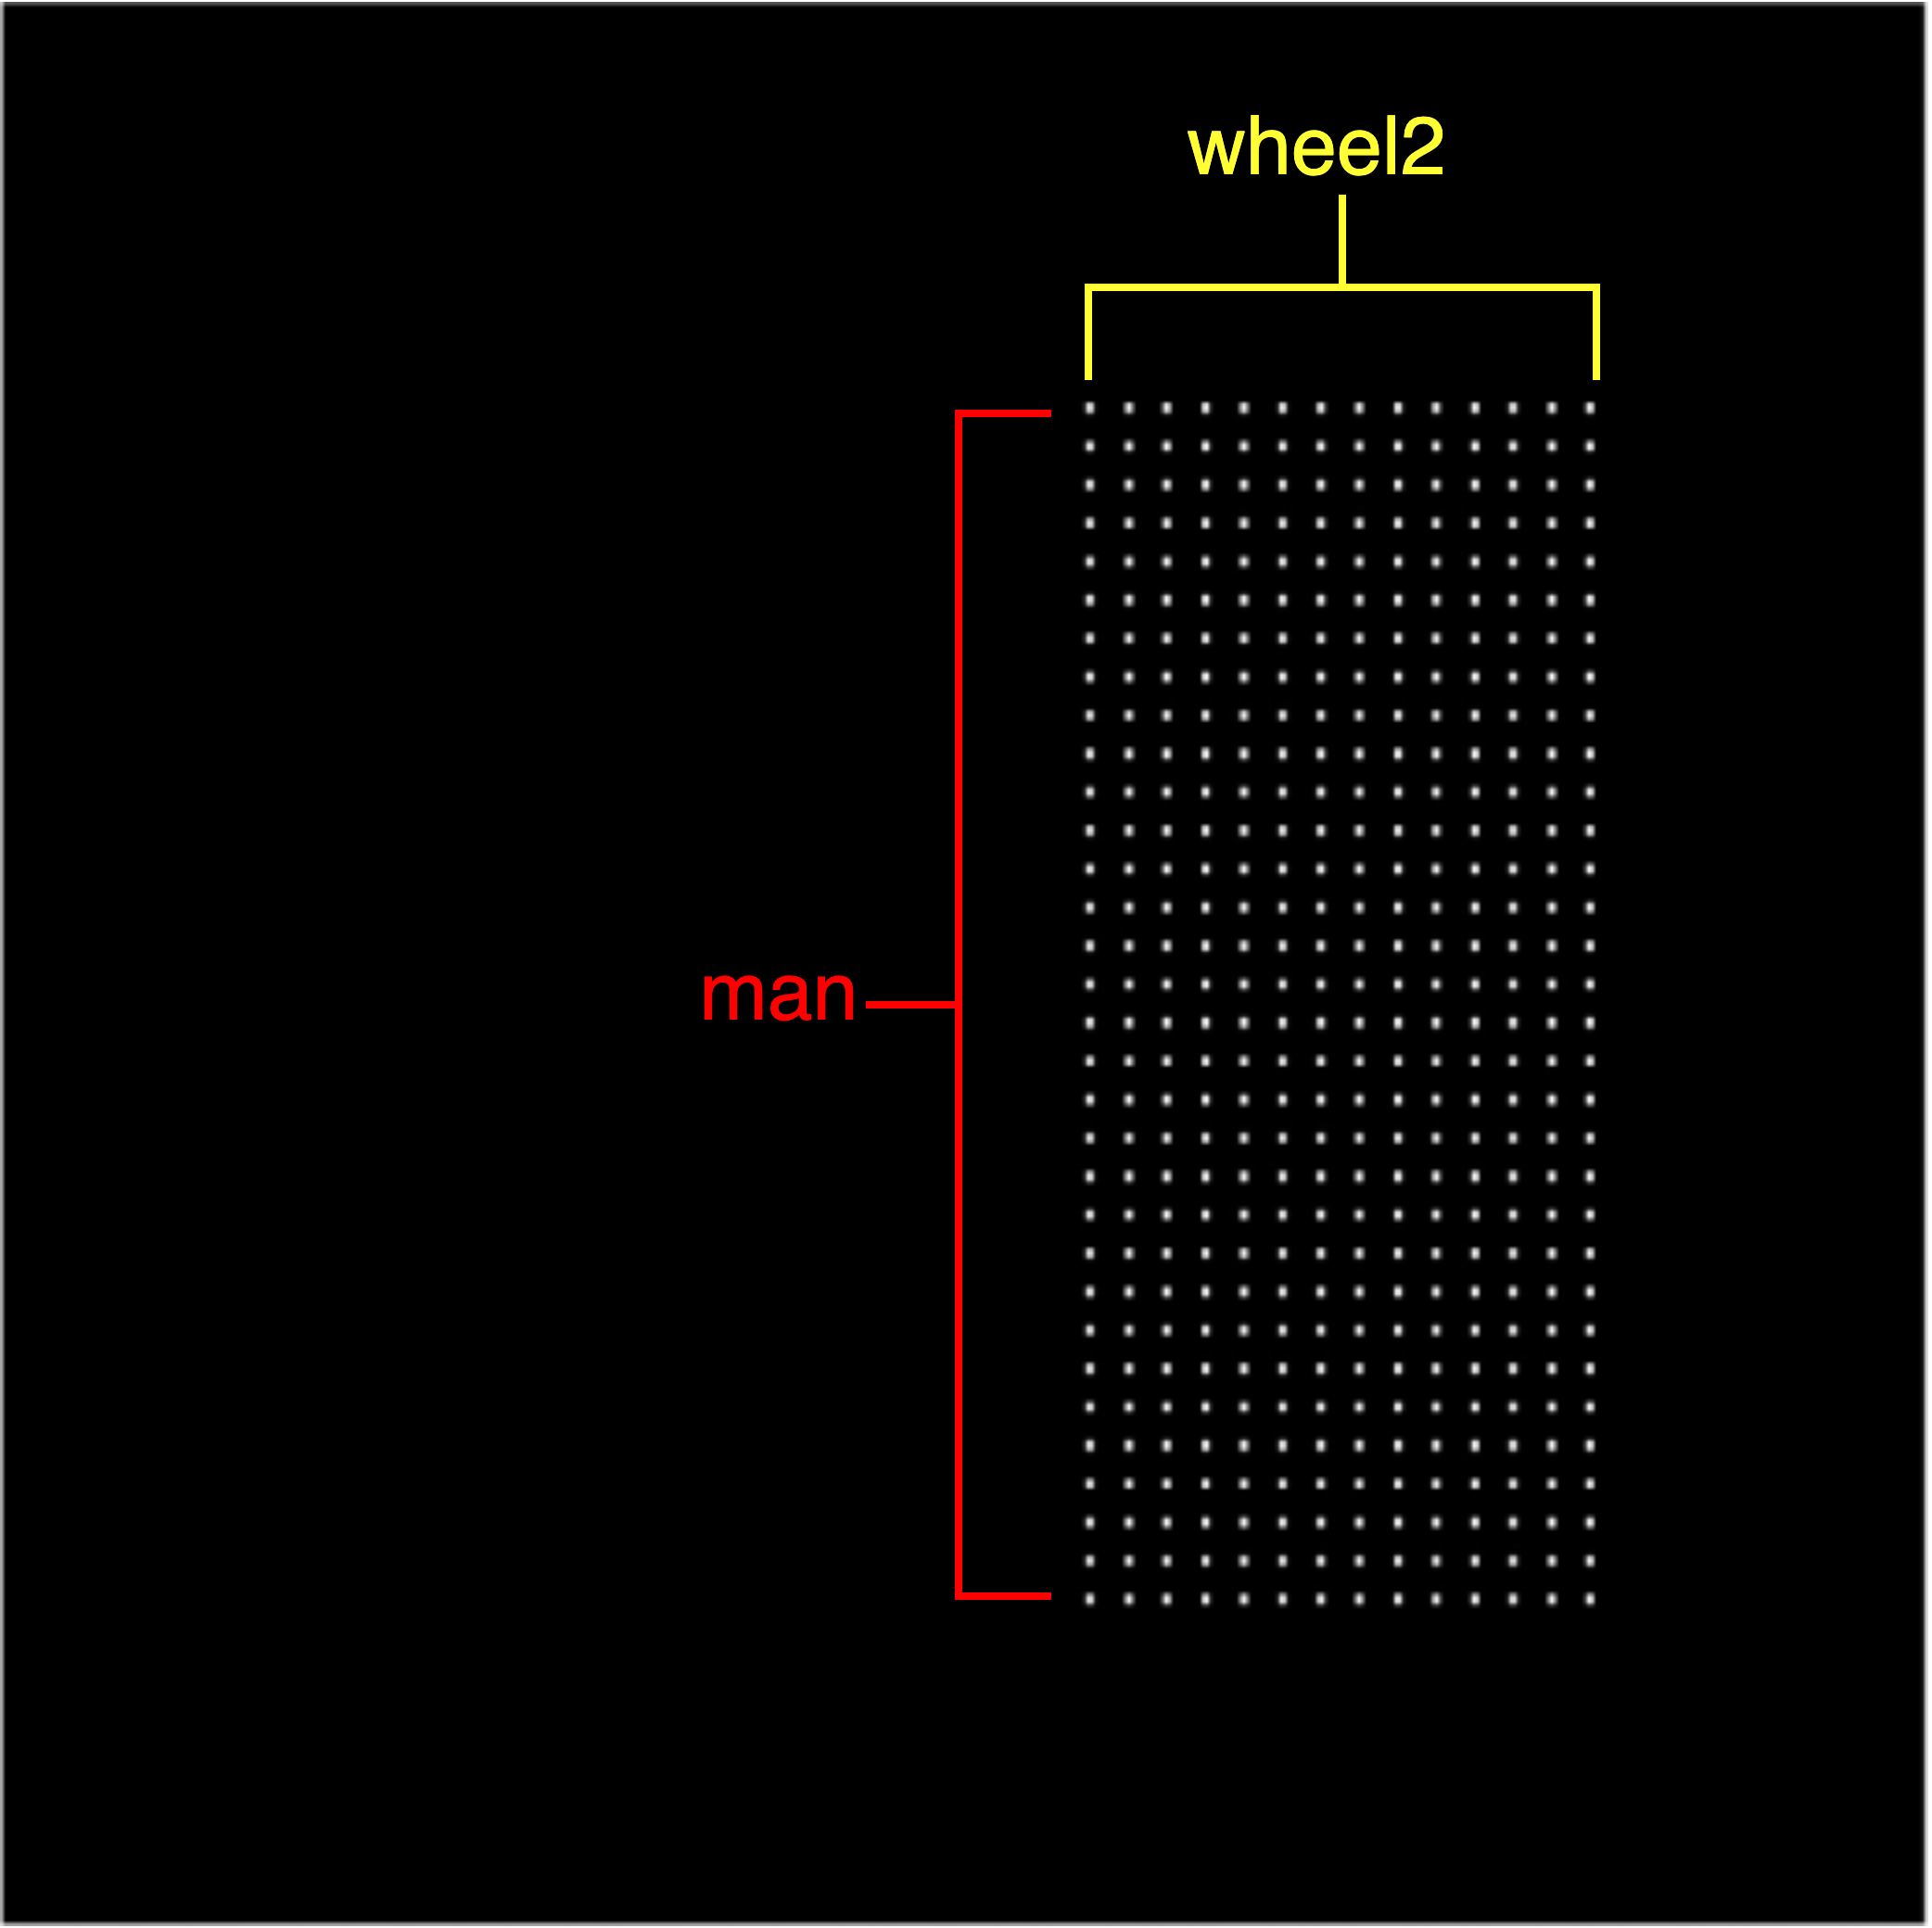
\includegraphics[width=0.9\linewidth]{figures/motor/map2}
			\label{fig:motor_map2}
	\end{minipage}}
	
	\caption[The attention map of each pair.]{The attention map of each pair, where $ (a) $ is the ground truth pair and $ (d) $ is its corresponding position in the attention map. $ (b) $, $(c) $ are no relationship pair, and $ (e) $, $ (f) $ is theirs corresponding positions in the attention map.}
	\label{fig:motor_pair}
\end{figure}

\begin{figure}[tbph!]
	\centering
	\subfigure[All pixels of $Att_{rel}$]{
		\begin{minipage}[t]{5cm}
			\centering
			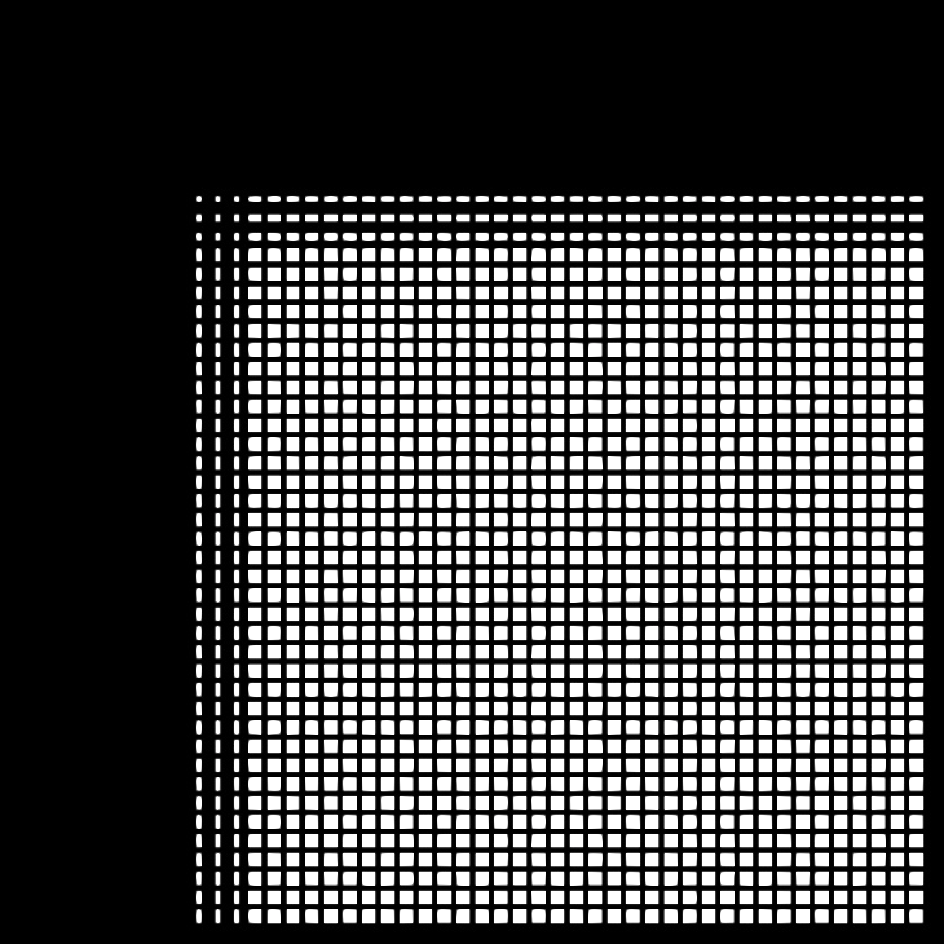
\includegraphics[width=0.9\linewidth]{figures/motor/all0}
			\label{fig:motor_all0}
	\end{minipage}}
	\subfigure[All pixels of $ Att_{no\_rel }$]{
		\begin{minipage}[t]{5cm}
			\centering
			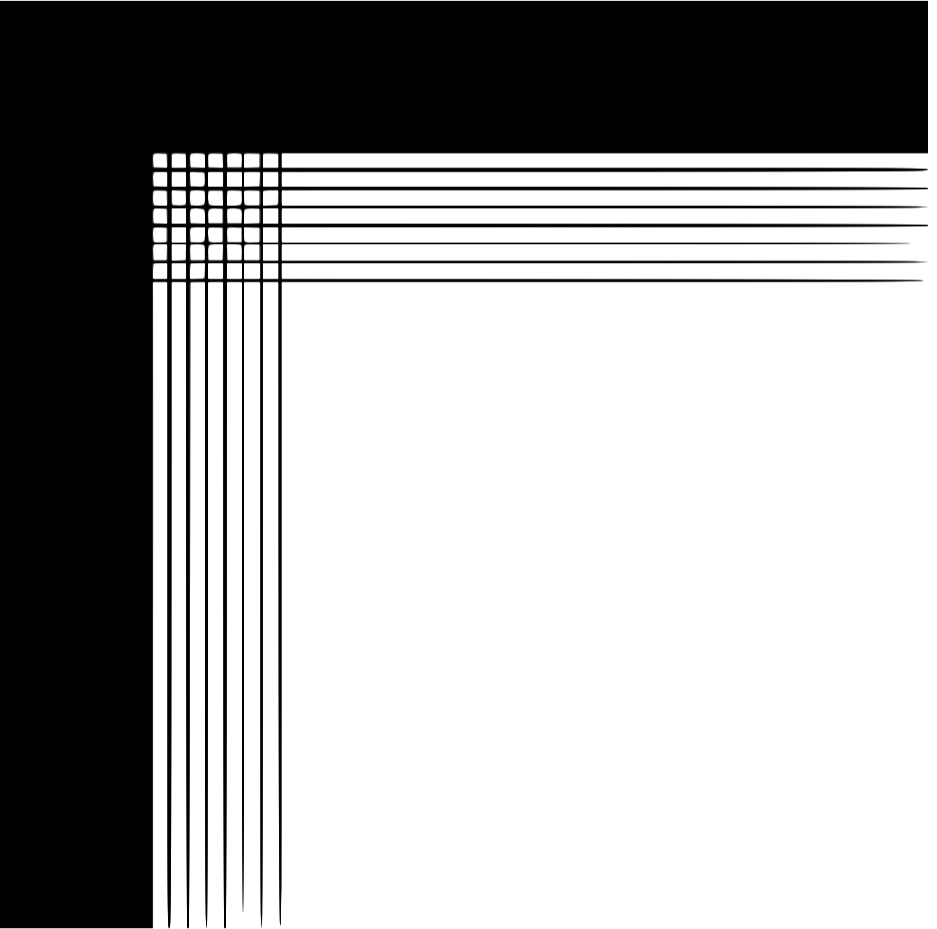
\includegraphics[width=0.9\linewidth]{figures/motor/all1}
			\label{fig:motor_all1}
	\end{minipage}}
	\subfigure[Overlap]{
		\begin{minipage}[t]{5cm}
			\centering
			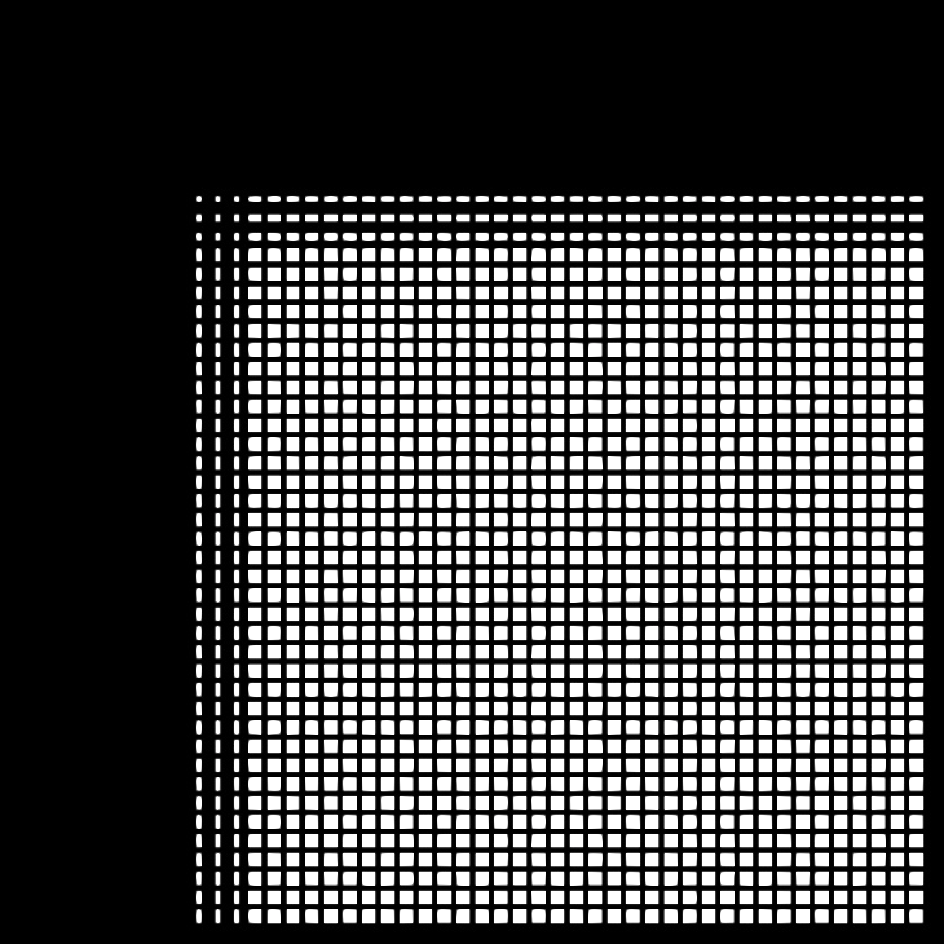
\includegraphics[width=0.9\linewidth]{figures/motor/all0}
			\label{fig:motor_all2}
	\end{minipage}}
	
	\caption[The overlap in Attention map]{The overlap in Attention map.The sub-figure (a) is the attention of all the related pairs, and the sub-figure (b) is the attention of all the irrelevant pairs. The sub-figure(c) shows that there is a serious overlap between them. We cannot increase the attention shown in (a) and decrease the attention of (b) through our attention loss.}
	\label{fig:overlap}
\end{figure}



\section{Experiments on Proposed Framework}

As mentioned above, our Pixel Attention idea did not meet our expectations due to the overlap. In this section, we introduce in detail the relevant experiments and results of our Retina Net.

\subsection{Implementation details}
We have implemented our model in $ pythorch\-0.4 $~\cite{paszke2019pytorch}. The input of our model is the same as~\cite{zellers2018neural} , that is an image with a size of $ 592 \times 592 $. We have used VGG16~\cite{simonyan2015deep} backbone pretrained on visual genome dataset. As mentioned in our Sec.~\ref{sec:retinanet}, the encoder and the two decoder modules accept input features of size 2048. We have used 3x Encoder, 3x Object Decoder , 3x Relation Decoder and 8 attention head for transformer network. The glove vector embedding has size 200. SGD with momentum along with learning rate of $ 10^{-3 }$ and our batch size is 6. Also, we have used cross-entropy loss for both of our object and relation classification loss.

We follow three standard evaluation modes same as in current benchmark of the Motifs-Net ~\cite{zellers2018neural}  : (1) \textbf{predicate classification} (PREDCLS): given a ground truth set of boxes and labels, predict relationship labels, (2) \textbf{scene graph classification} (SGCLS): given ground truth boxes, predict box labels and relationship label and (3) \textbf{scene graph detection} (SGDET): predict boxes, box labels, and relationship labels.
For the subtask SGDET, we use a learnable object query, and use the Hungarian matching algorithm to match each object feature. For the other two subtasks, we use our custom object query to obtain the object feature.


\subsection{Experiment on Object query}

We will discuss the feasibility of our proposed object query to replace learnable query. The task PredClS has classes and bounding boxes information, so we designed several object queries based on the known information, as shown in Fig.~\ref{fig:objectquery}, Fig.~\ref{fig:objquery1} and Fig.~\ref{fig:objquery2}. We call them  \textit{objec query 1} ,  \textit{objec query 2} , and  \textit{objec query 3}  respectively. We will discuss their pros and cons, and their substitutability.

We have already mentioned object query 1 above, it has the spatial information of the entity, while the object query 2 is to add a class word embedding on his basis, so that our object query has semantic information. For the object query 3, we only made a simple design. The bounding box of each entity in a picture is different, so their object query is also different.

\begin{figure}[tbph!]
	\centering
	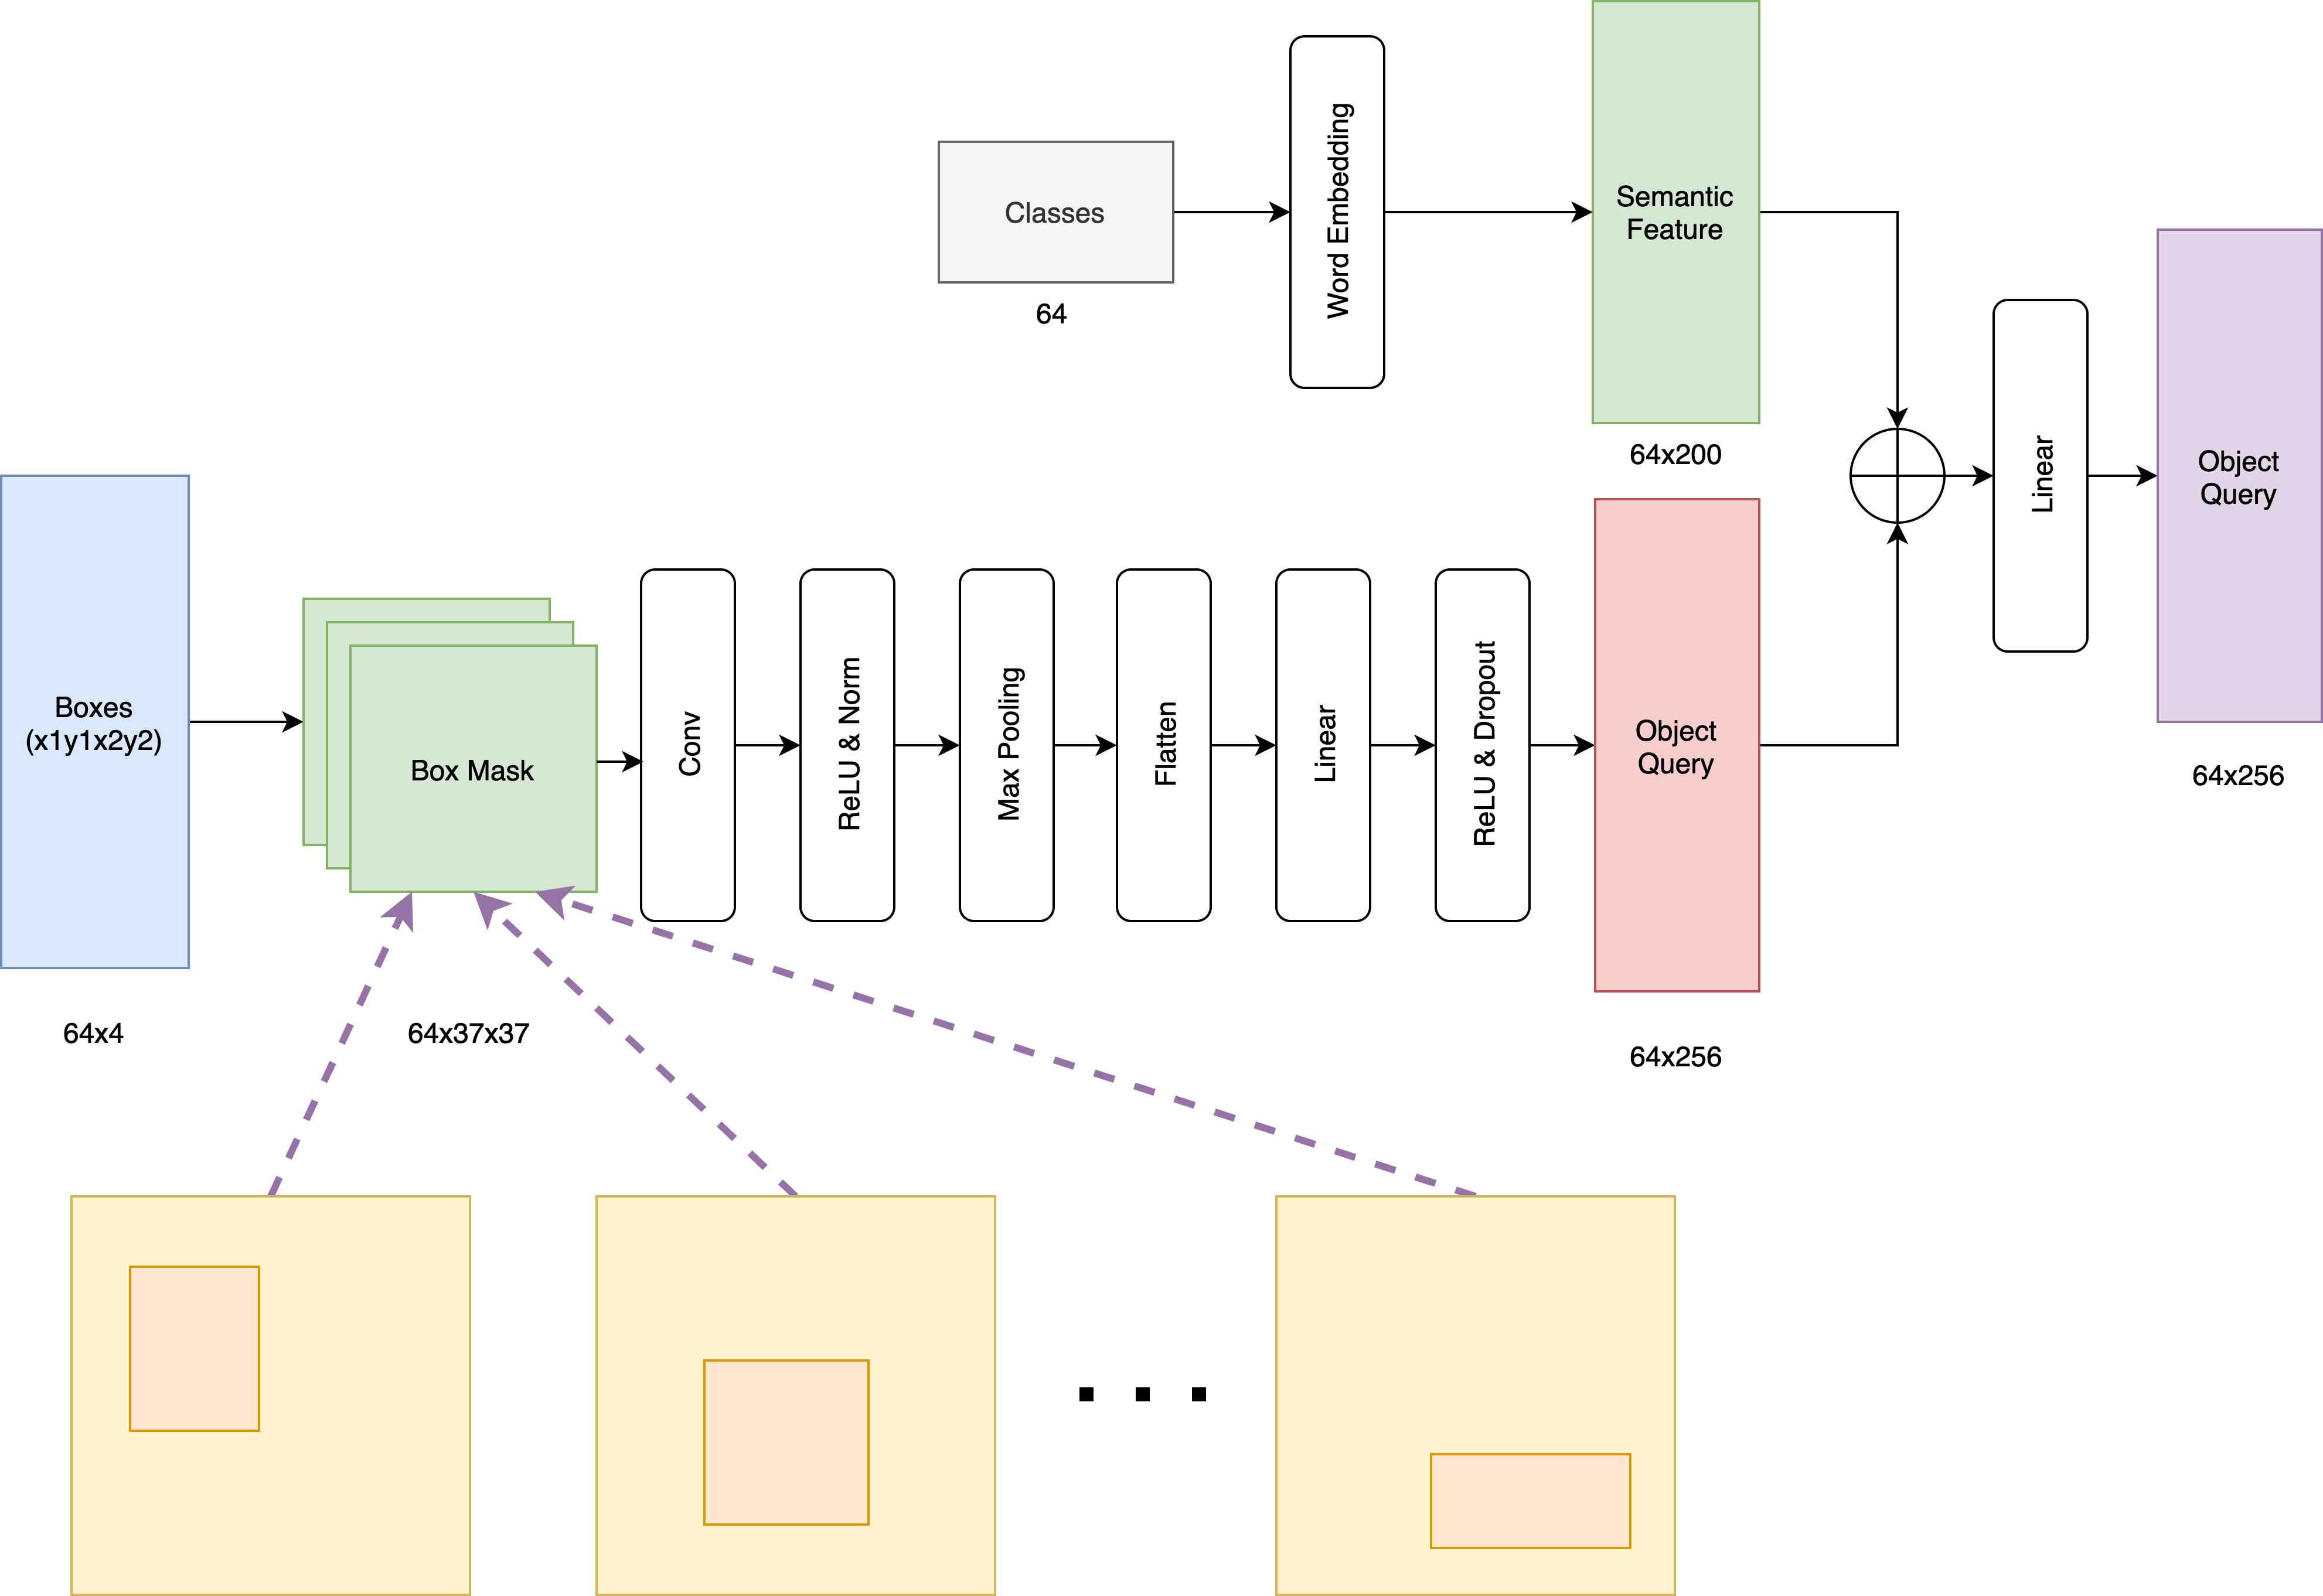
\includegraphics[width=0.9\linewidth]{figures/obj_query1}
	\caption[Illutrastion of the object query 2]{Illutrastion of the object query 2. Compared with object query1, we integrate the semantic feature of objects.}
	\label{fig:objquery1}
\end{figure}

\begin{figure}[tbph!]
	\centering
	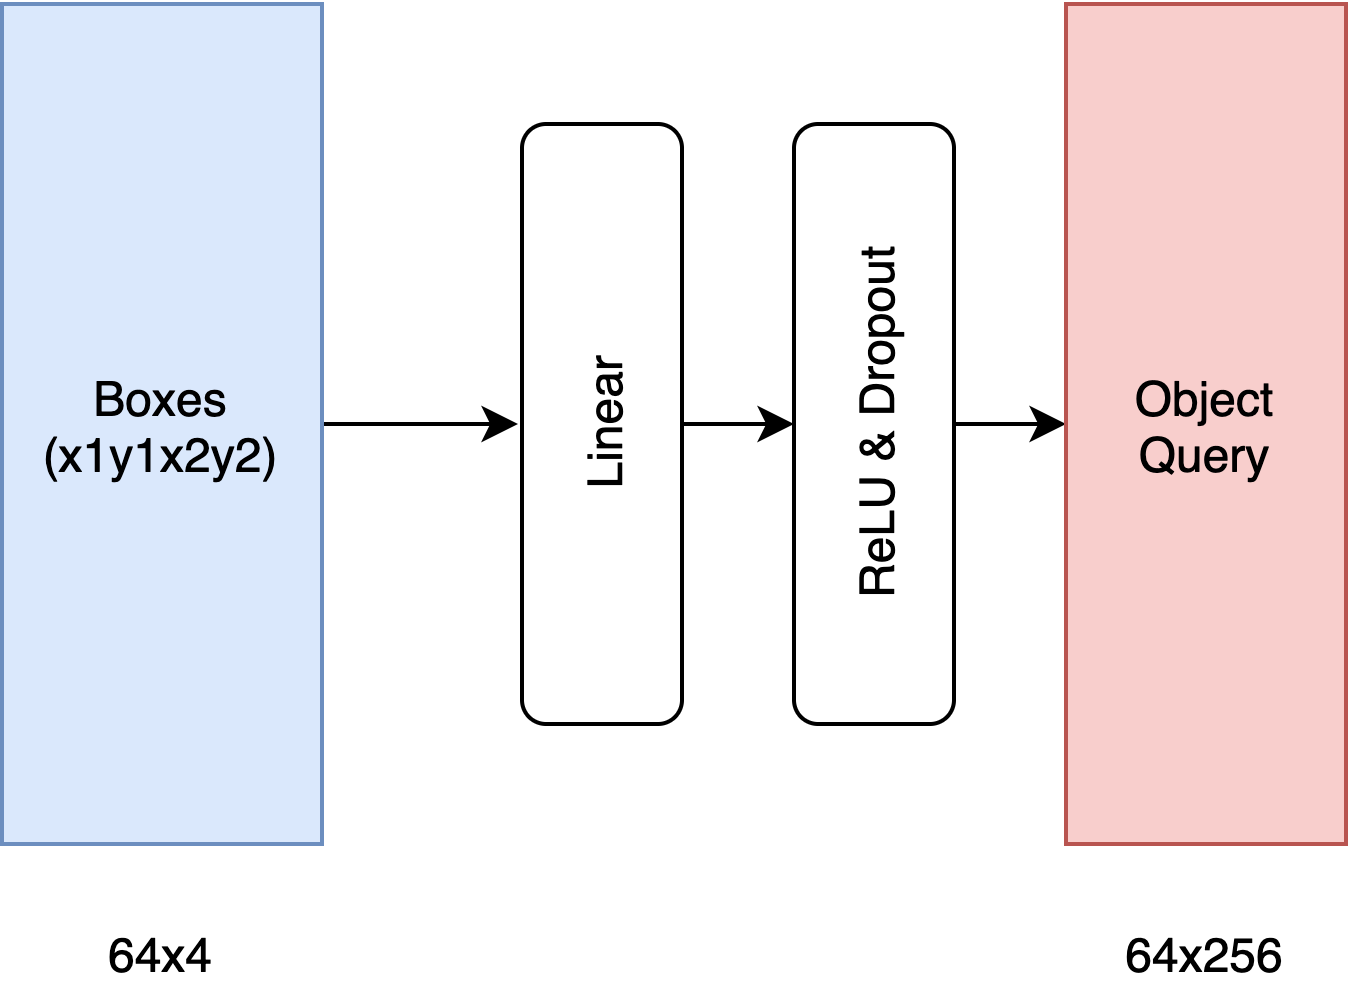
\includegraphics[width=0.5\linewidth]{figures/obj_query2}
	\caption[Illutrastion of the object query 3]{Illutrastion of the object query 3,we only added a simple linear layer behind the bounding box.}
	\label{fig:objquery2}
\end{figure}

\subsubsection{Consistency of the Object Query }

When people use a learnable embedding vector as the query, such as detr, they need to use the Hungarian matching algorithm to find the most matching object feature, because their query has no actual physical meaning. And our object query contains relevant information of each object, such as spatial information and semantic information. He is in one-to-one correspondence with the entities in the picture.

In order to verify the correspondence between our object query and the entity in the picture, we designed a regression experiment: we add an Multilayer Perceptron(MLP) module after ours object query and object feaure, then observe whether they can regain the spatial information of the object. We use IoU and GIoU~\cite{rezatofighi2019generalized}  as evaluation metrics.

After the MLP we obtain a bounding box tenser $ \hat{b_\sigma} $, then we calculate the box loss $\mathcal{L}_{box}$ with ground truth bounding box $b$, it consists of a GIoU loss and a $l_1$ loss, see the following equation:

$$ \mathcal{L}_{box}(b,\hat{b}_{\hat{\sigma}}) = \mathcal{L}_{GIoU}(b,\hat{b}_{\sigma}) + \left \| b - \hat{b}_{\sigma}  \right \| _1 $$

\begin{table}[!h]
	\centering
	\begin{tabular}{c|ccc}
		\bottomrule
		& object query 1 & object query 2 & object query 3  \\ \midrule
		IoU  & 0.759  & 0.750  & 0.681    \\
		GIoU & 0.744  & 0.733 & 0.669   \\ \bottomrule
		&object feature 1  &object feaure 2 & object feautre 3\\ \midrule
		IoU & 0.634 & 0.631 & 0.580 \\
		GIoU	& 0.617 & 0.620 & 0.568  \\\bottomrule
		
	\end{tabular}
\caption[The regression result of the object query and feature]{The regression result of the object query and feature.}
\label{tab:regresstion}
\end{table}

We can summarize from Tab~\ref{tab:regresstion} that our object query corresponds to object, and the IoU can reach about 75\%., and its  generated features also have about 60\%  IoU.

\subsubsection{Visualization of our object query}
Our object query is a $ 64 \times 256 $ tensor, corresponding to objects in each image, so we can draw each object query into a size of $16 \times 16$ image, see Fig.~\ref{fig:tennis} and Fig.~\ref{fig:street}. 

From the figure, we can see that we have generated three different queries through three different methods, and the query corresponding to each object is also different. For example, our object query1, as the area of our entities gradually increases, our query gradually becomes denser. 


\begin{figure}[h!]
	\centering
	\subfigure[The objects with bounding boxes.]{
		\begin{minipage}[t]{3.5cm}
			\centering
			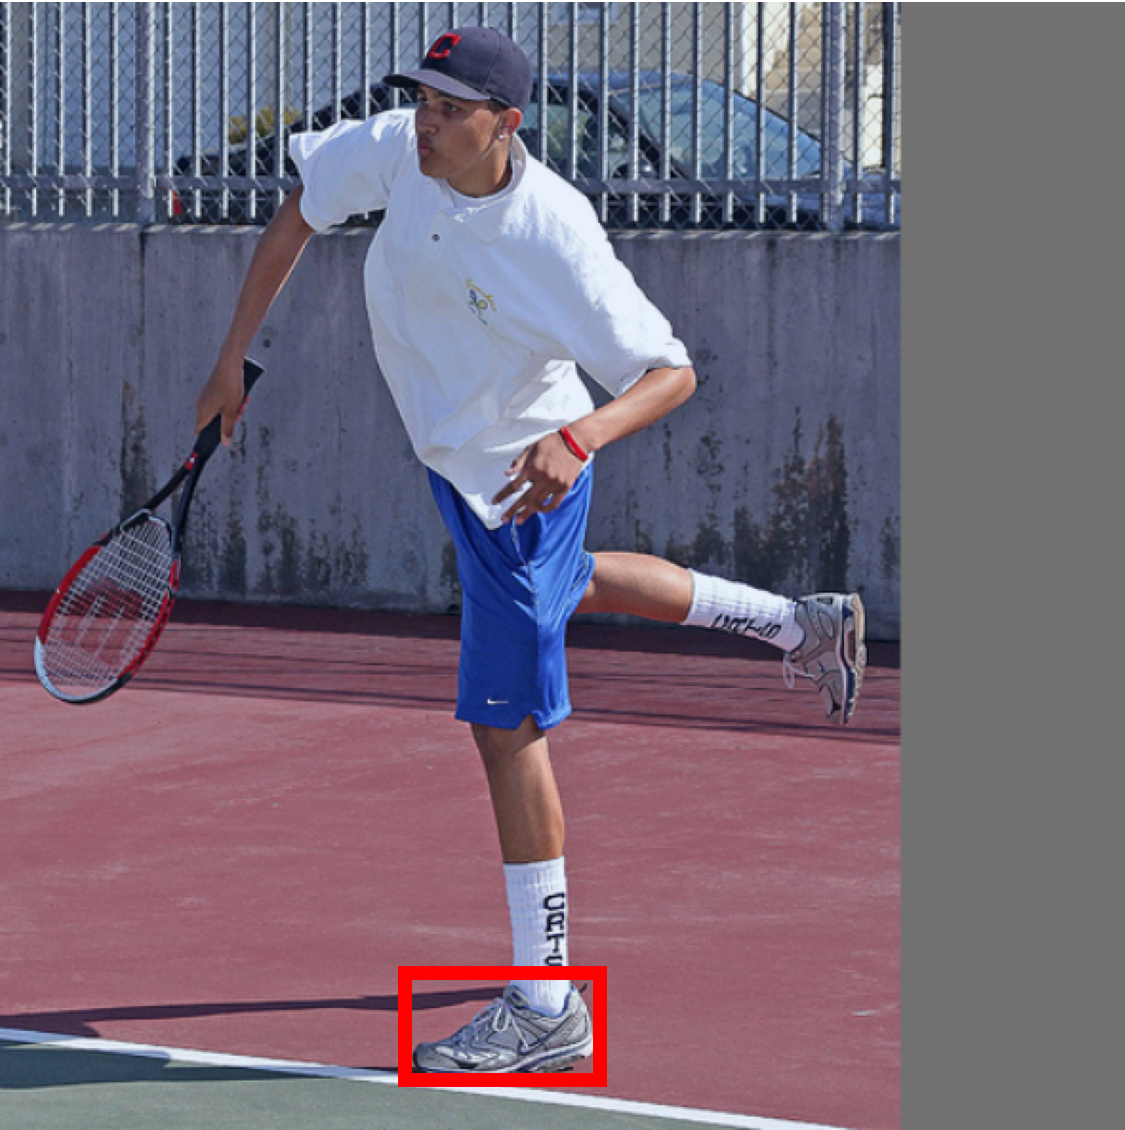
\includegraphics[width=0.9\linewidth]{figures/result/tennis/obj2}
	\end{minipage}
		\begin{minipage}[t]{3.5cm}
			\centering
			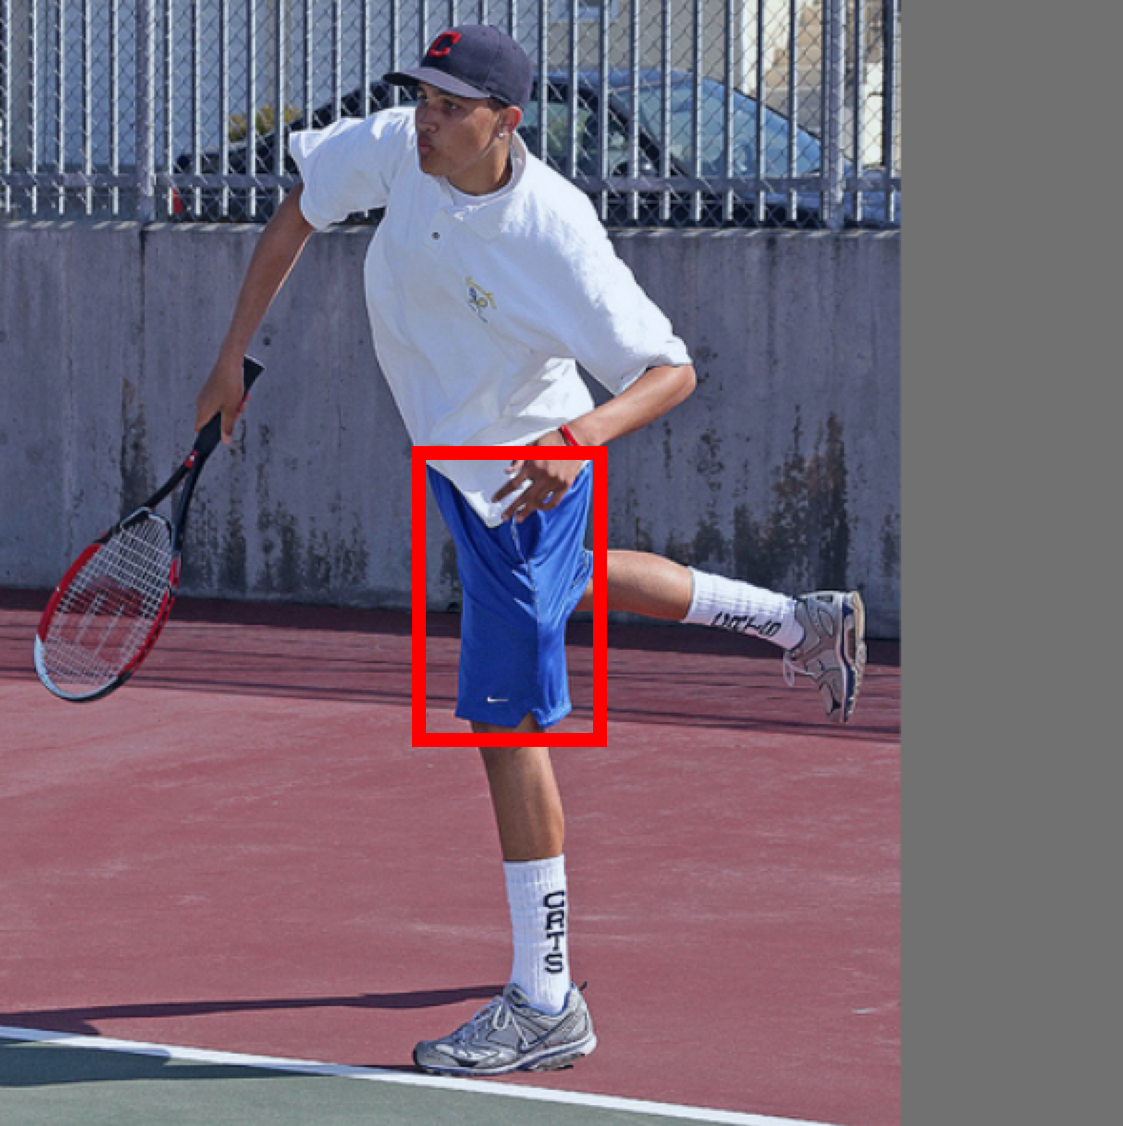
\includegraphics[width=0.9\linewidth]{figures/result/tennis/obj4}
	\end{minipage}
	\begin{minipage}[t]{3.5cm}
		\centering
		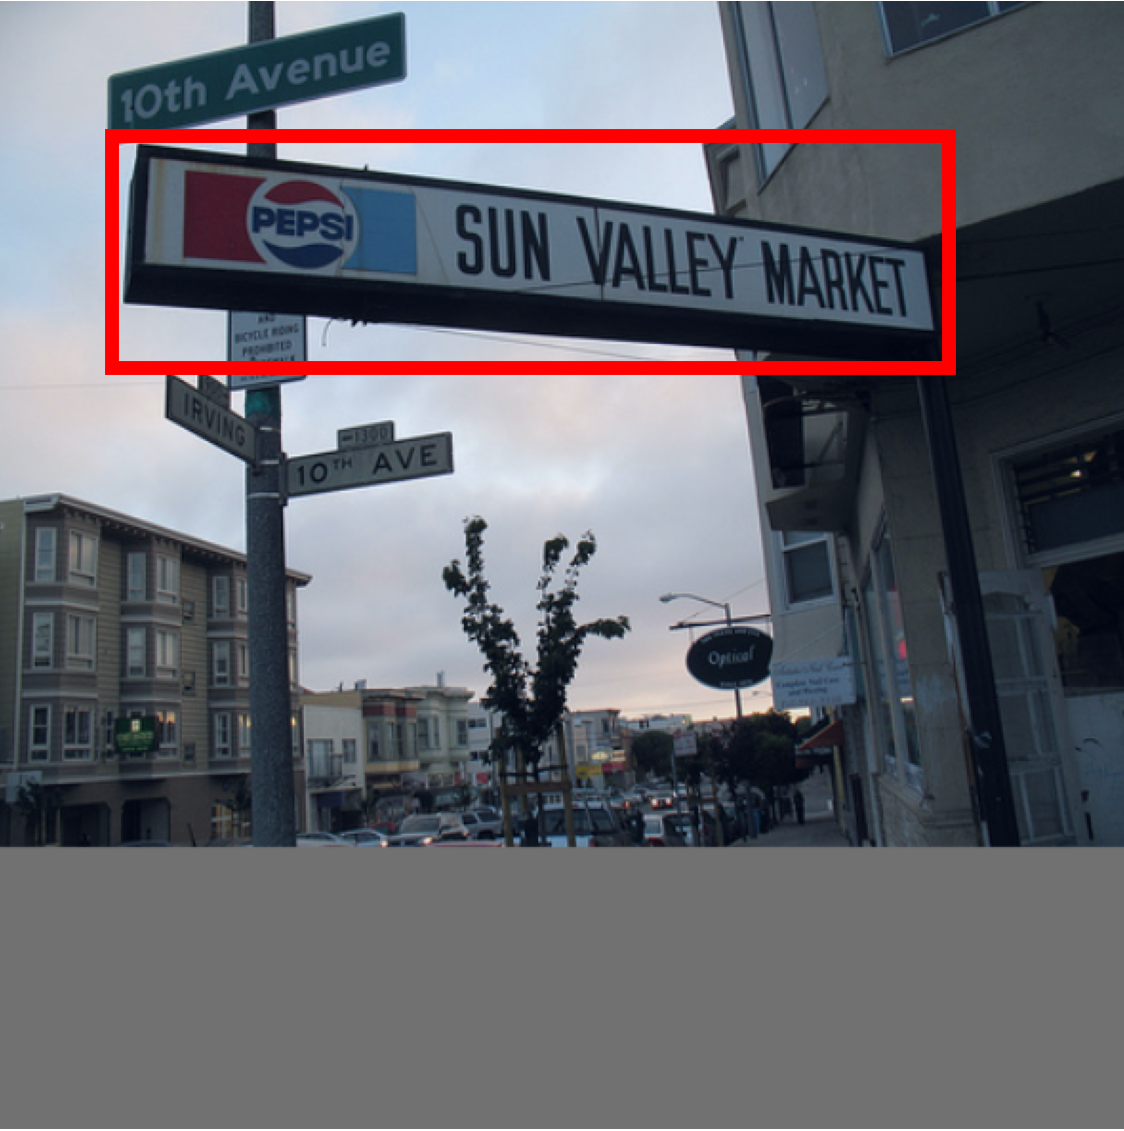
\includegraphics[width=0.9\linewidth]{figures/result/street/o3}
	\end{minipage}
		\begin{minipage}[t]{3.5cm}
			\centering
			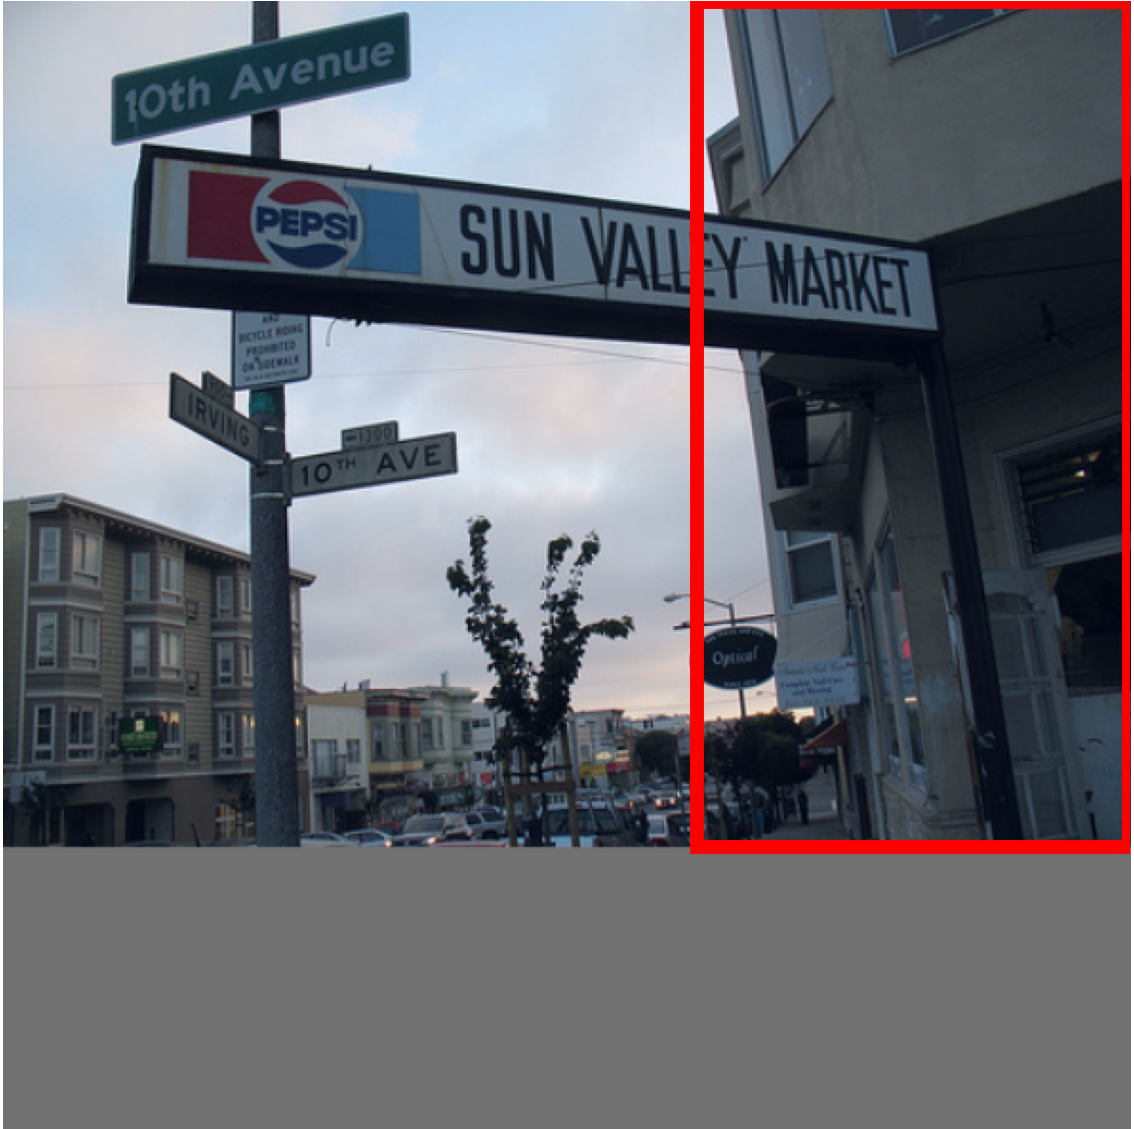
\includegraphics[width=0.9\linewidth]{figures/result/street/o4}
	\end{minipage}}
	
	\subfigure[The object query 1.]{
		\begin{minipage}[t]{3.5cm}
			\centering
			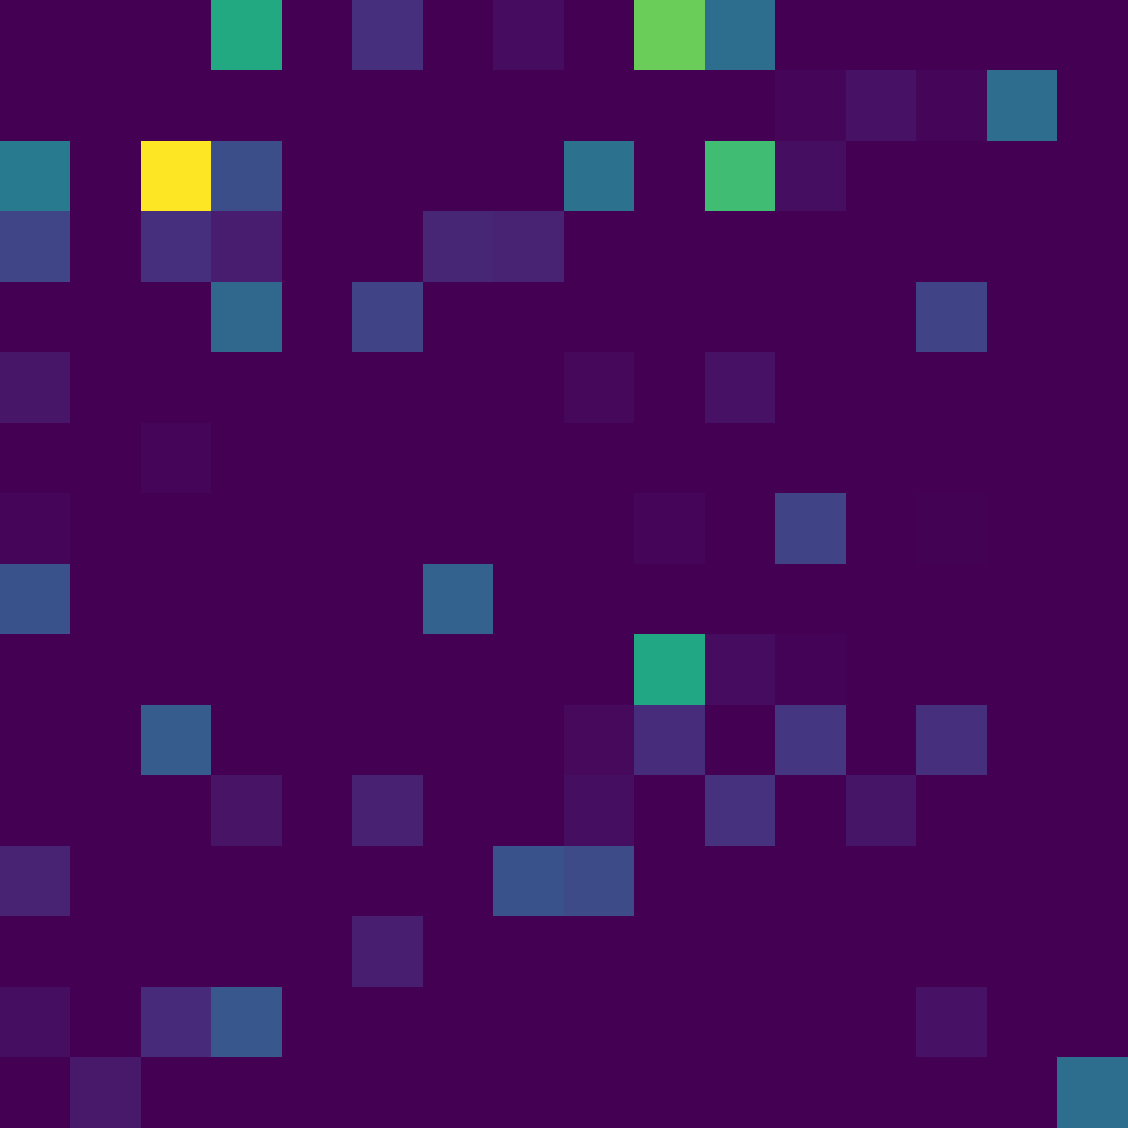
\includegraphics[width=0.9\linewidth]{figures/result/tennis/q0_2}
	\end{minipage}
		\begin{minipage}[t]{3.5cm}
			\centering
			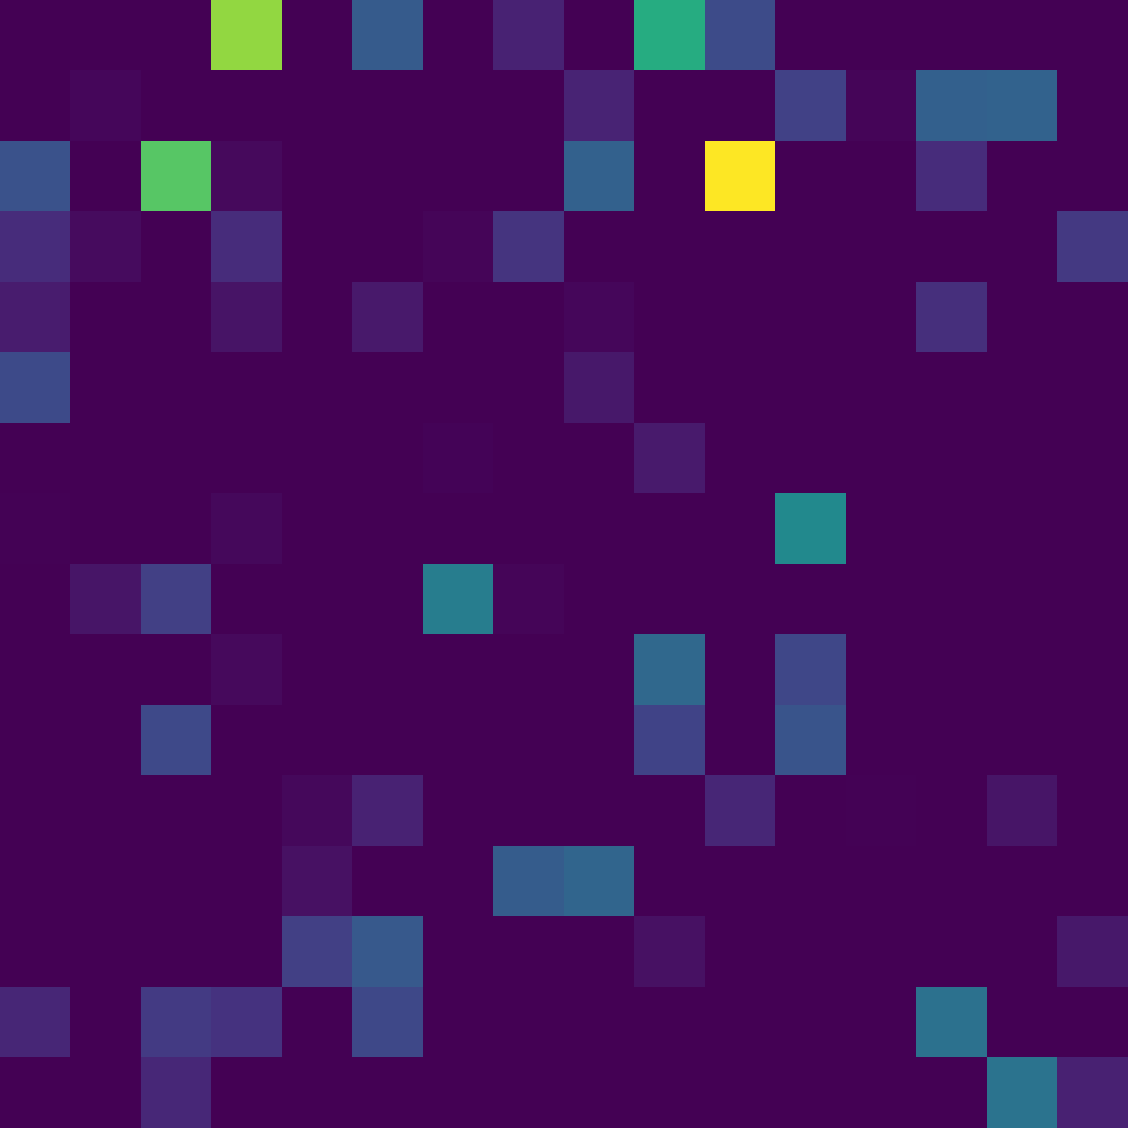
\includegraphics[width=0.9\linewidth]{figures/result/tennis/q0_4}
	\end{minipage}
	\begin{minipage}[t]{3.5cm}
		\centering
		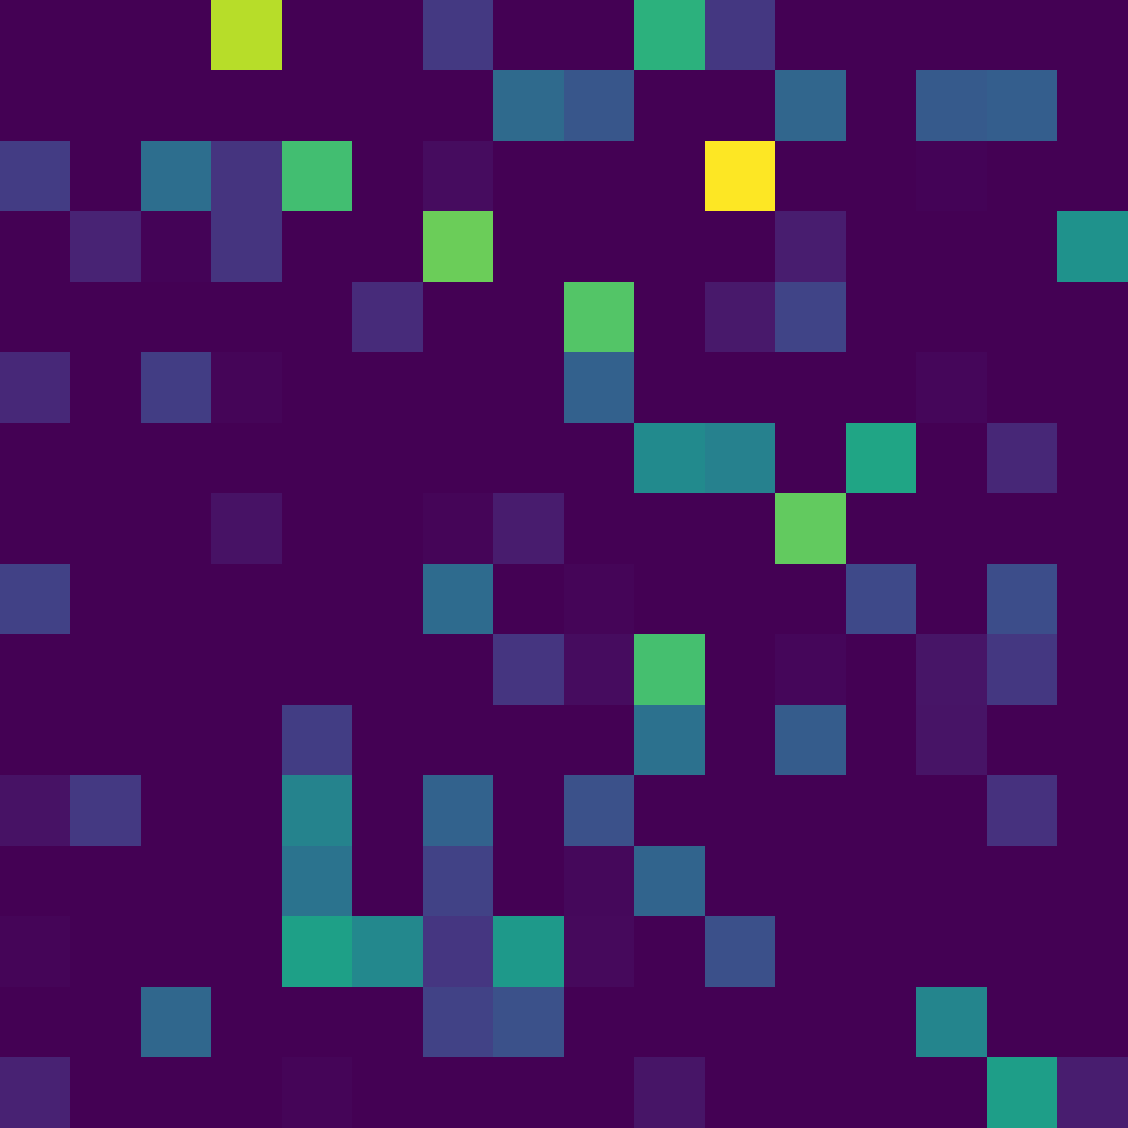
\includegraphics[width=0.9\linewidth]{figures/result/street/q0_3}
	\end{minipage}
		\begin{minipage}[t]{3.5cm}
			\centering
			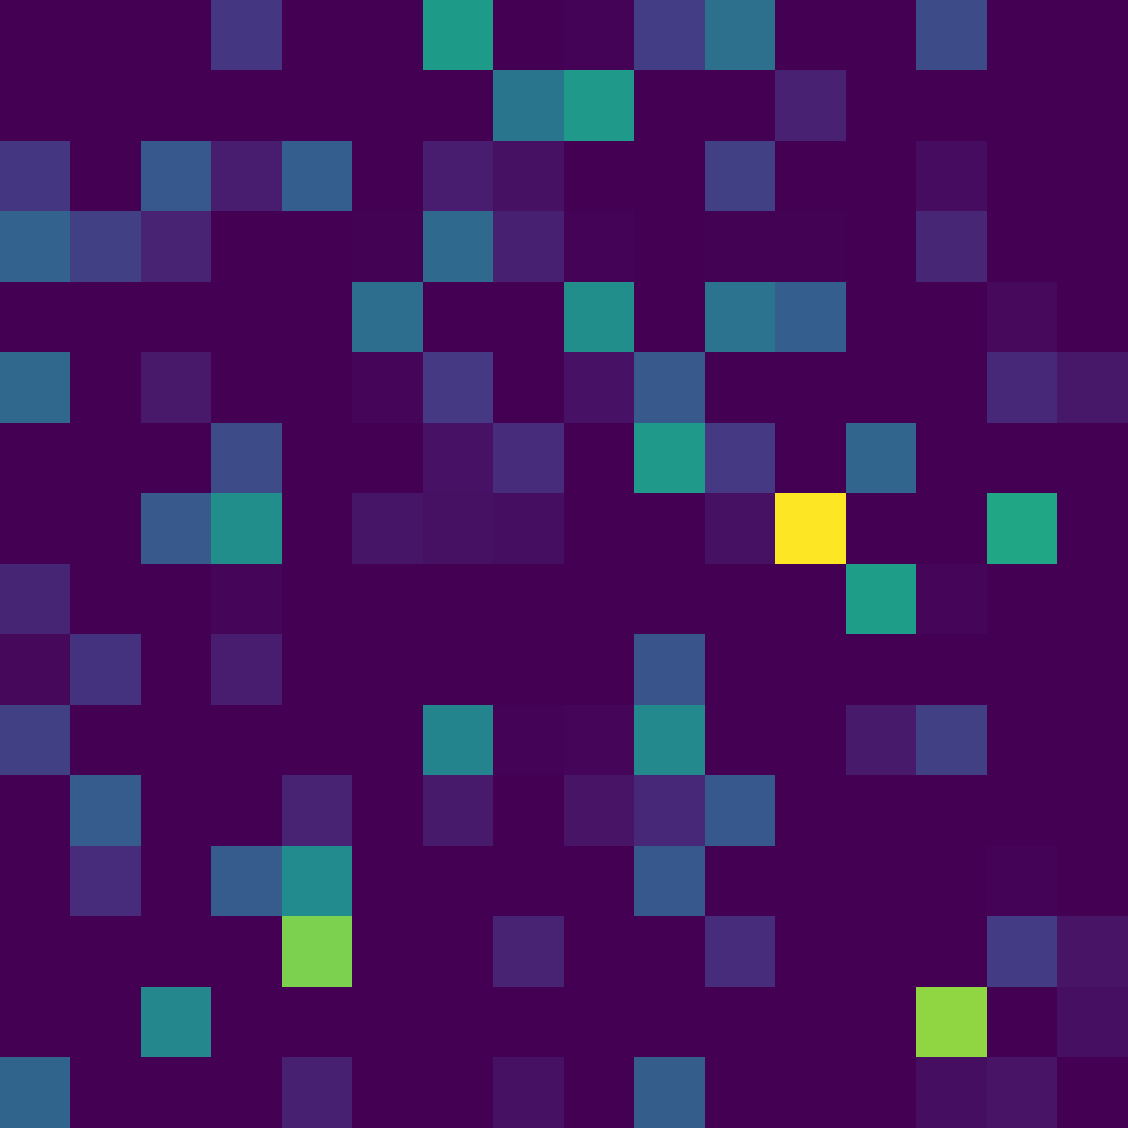
\includegraphics[width=0.9\linewidth]{figures/result/street/q0_4}
	\end{minipage}}


		\subfigure[the object query 2.]{
		\begin{minipage}[t]{3.5cm}
			\centering
			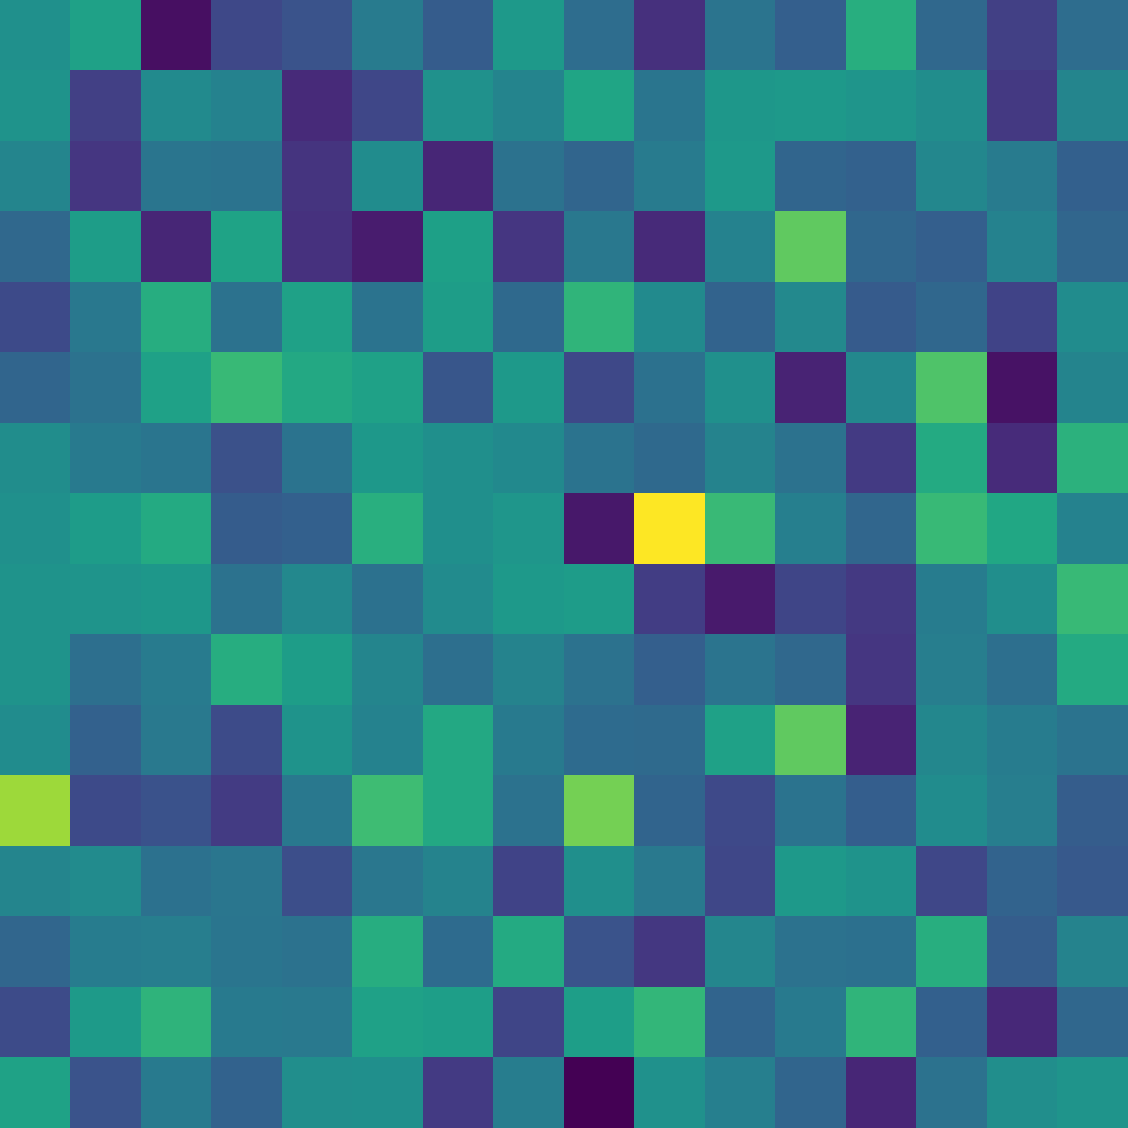
\includegraphics[width=0.9\linewidth]{figures/result/tennis/q3_2}
	\end{minipage}
		\begin{minipage}[t]{3.5cm}
			\centering
			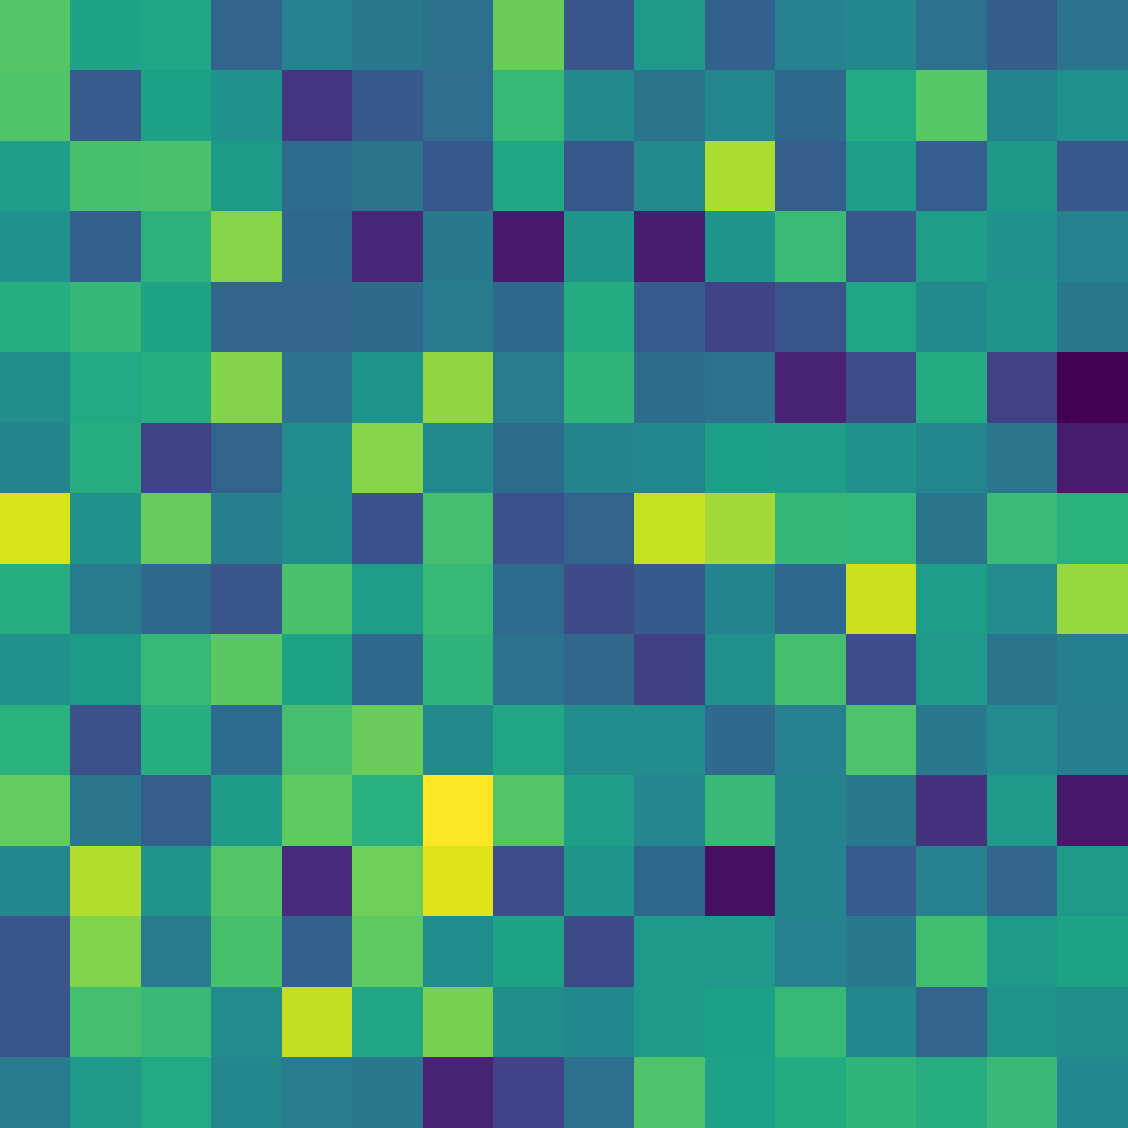
\includegraphics[width=0.9\linewidth]{figures/result/tennis/q3_4}
	\end{minipage}
		\begin{minipage}[t]{3.5cm}
			\centering
			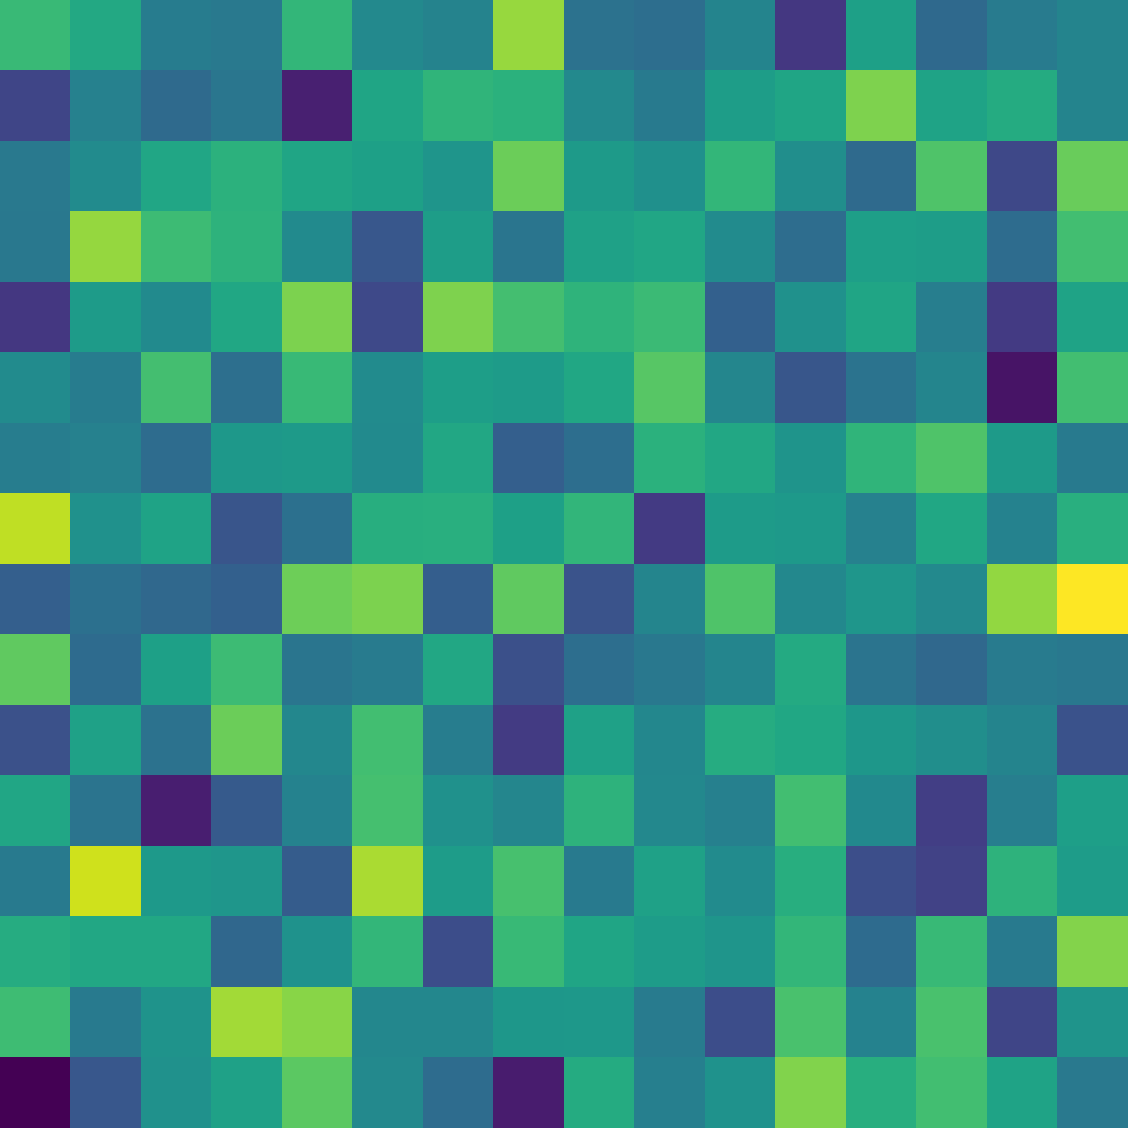
\includegraphics[width=0.9\linewidth]{figures/result/street/q3_3}
	\end{minipage}
		\begin{minipage}[t]{3.5cm}
			\centering
			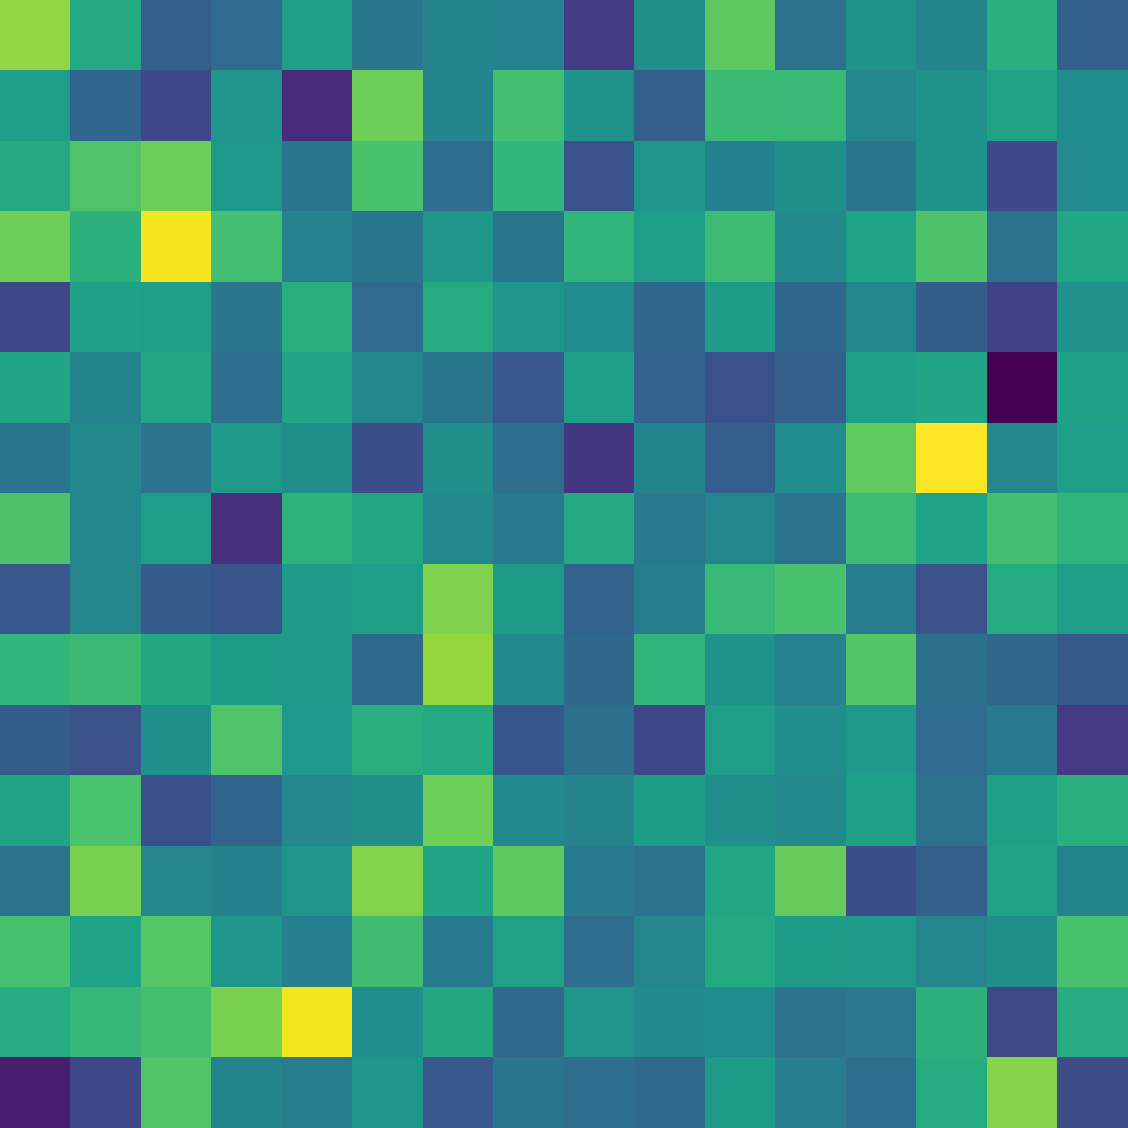
\includegraphics[width=0.9\linewidth]{figures/result/street/q3_4}
	\end{minipage}}

	\subfigure[The object query 3.]{
		\begin{minipage}[t]{3.5cm}
			\centering
			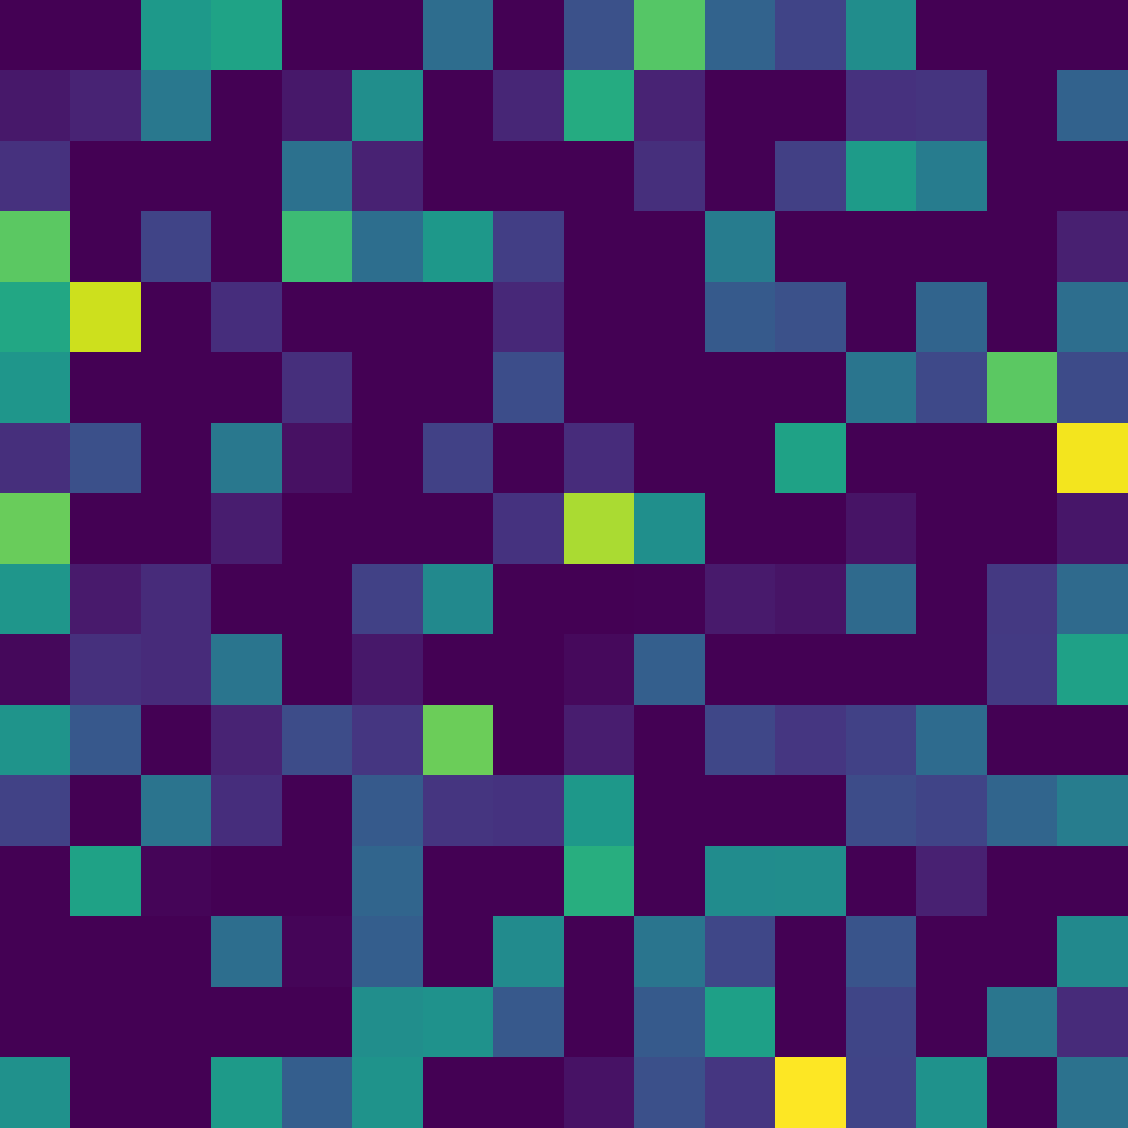
\includegraphics[width=0.9\linewidth]{figures/result/tennis/q2_2}
	\end{minipage}
		\begin{minipage}[t]{3.5cm}
			\centering
			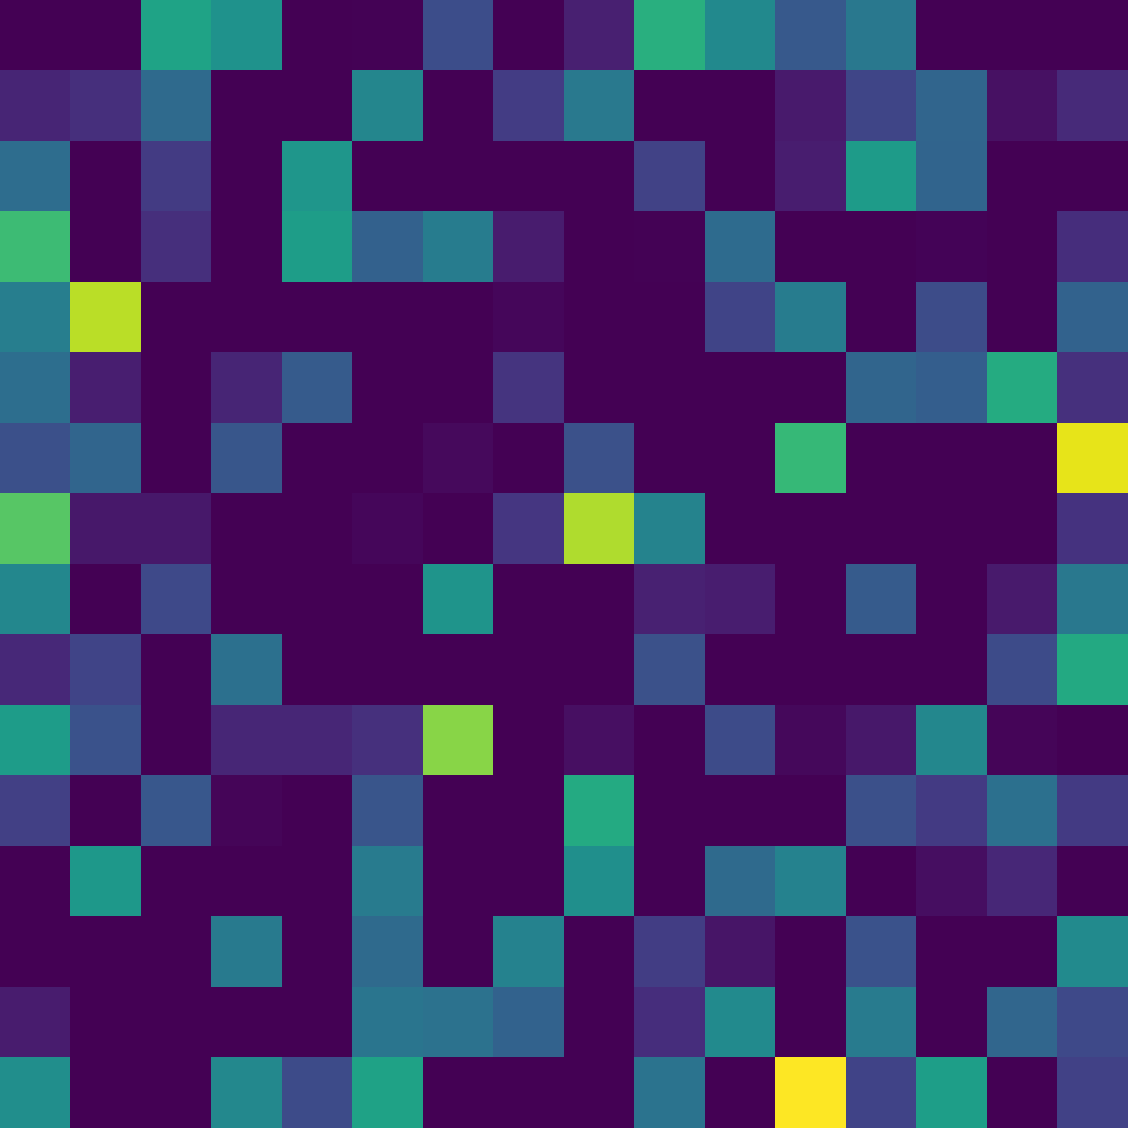
\includegraphics[width=0.9\linewidth]{figures/result/tennis/q2_4}
	\end{minipage}
	\begin{minipage}[t]{3.5cm}
	\centering
	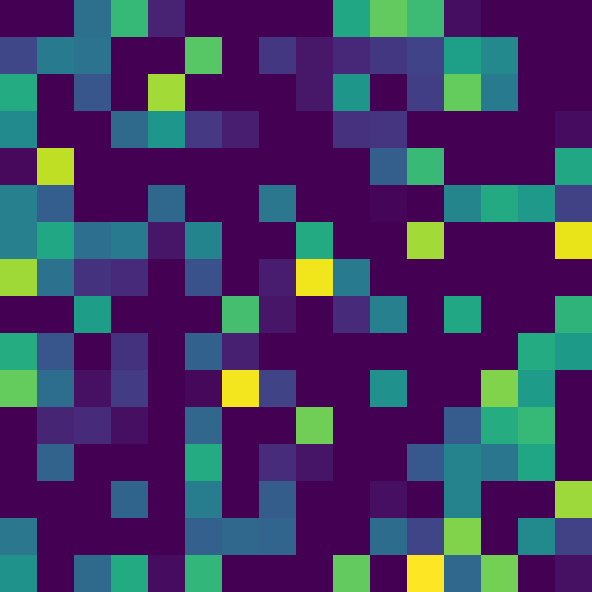
\includegraphics[width=0.9\linewidth]{figures/result/street/q2_3}
	\end{minipage}
	\begin{minipage}[t]{3.5cm}
	\centering
	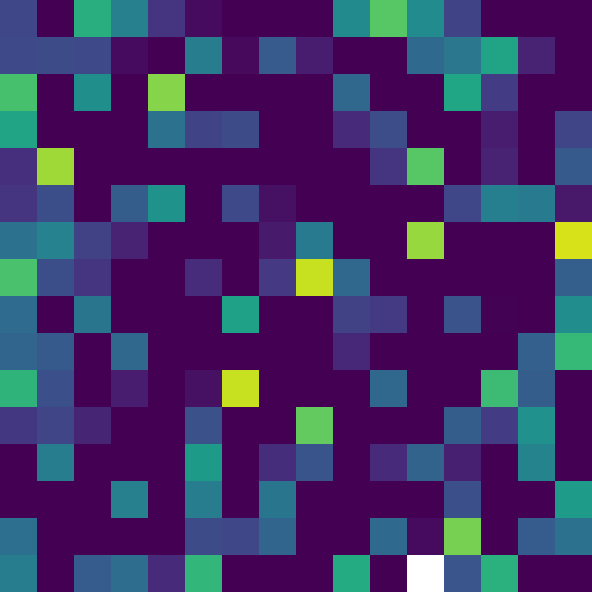
\includegraphics[width=0.9\linewidth]{figures/result/street/q2_4}
	\end{minipage}}

	\caption[An instance of Visualized results of the object query]{An instance of visualized results of the object query.from top to bottom, each row represents the position of the object, object query 1, object query 2 and object query 3.}
	\label{fig:tennis}
\end{figure}

\subsubsection{Result of our object query}
Next, we use our object query as the input of the object decoder to test the performance of these three queries in the task PredCLS, and we use recall@50 and recall@100 as the criterion.We can see the results in Table~\ref{tab:result_object _query}.

\begin{table}[!h]
	\centering
	\begin{tabular}{c|ccc}
		\hline
		& object query 1 & object query 2 & object query 2 \\ \hline
		Recall@50  & 62.9            & 63.2            & 63.0              \\
		Recall@100 & 65.0             & 65.3              & 65.1              \\ \hline
	\end{tabular}

\caption[The result of object query in PredCLS]{The result of object query in PredCLS.}
\label{tab:result_object _query}
\end{table}

According to the above table, the performance of the three object queries in PredCLS is similar. Based on the previous results, we draw the following conclusions:

\begin{enumerate}
	\item The object query and object feature we designed correspond to each other, which can replace learnable query and solve the VRD problem.
	\item Different object query designs are not very helpful to the VRD problem. We only need to design a query that can distinguish each object, that is, each query needs to correspond to each entity one by one.
\end{enumerate}


\subsection{Experiment on Attention  Loss Function}

We designed an attention loss to make our object feature better. In this part, we designed some experiments to verify its effect.

The Figure~\ref{fig:attention_loss_result} is the training result of our attention loss. We record a loss every 100 step, sum up 1000 data, and use matlab to perform low-pass filtering to draw the result. We found that our attention from the beginning $ 10^{-4} $ dropped rapidly and gradually tended to 0 in the process of about 500 steps.

\begin{figure}[h!]
	\centering
	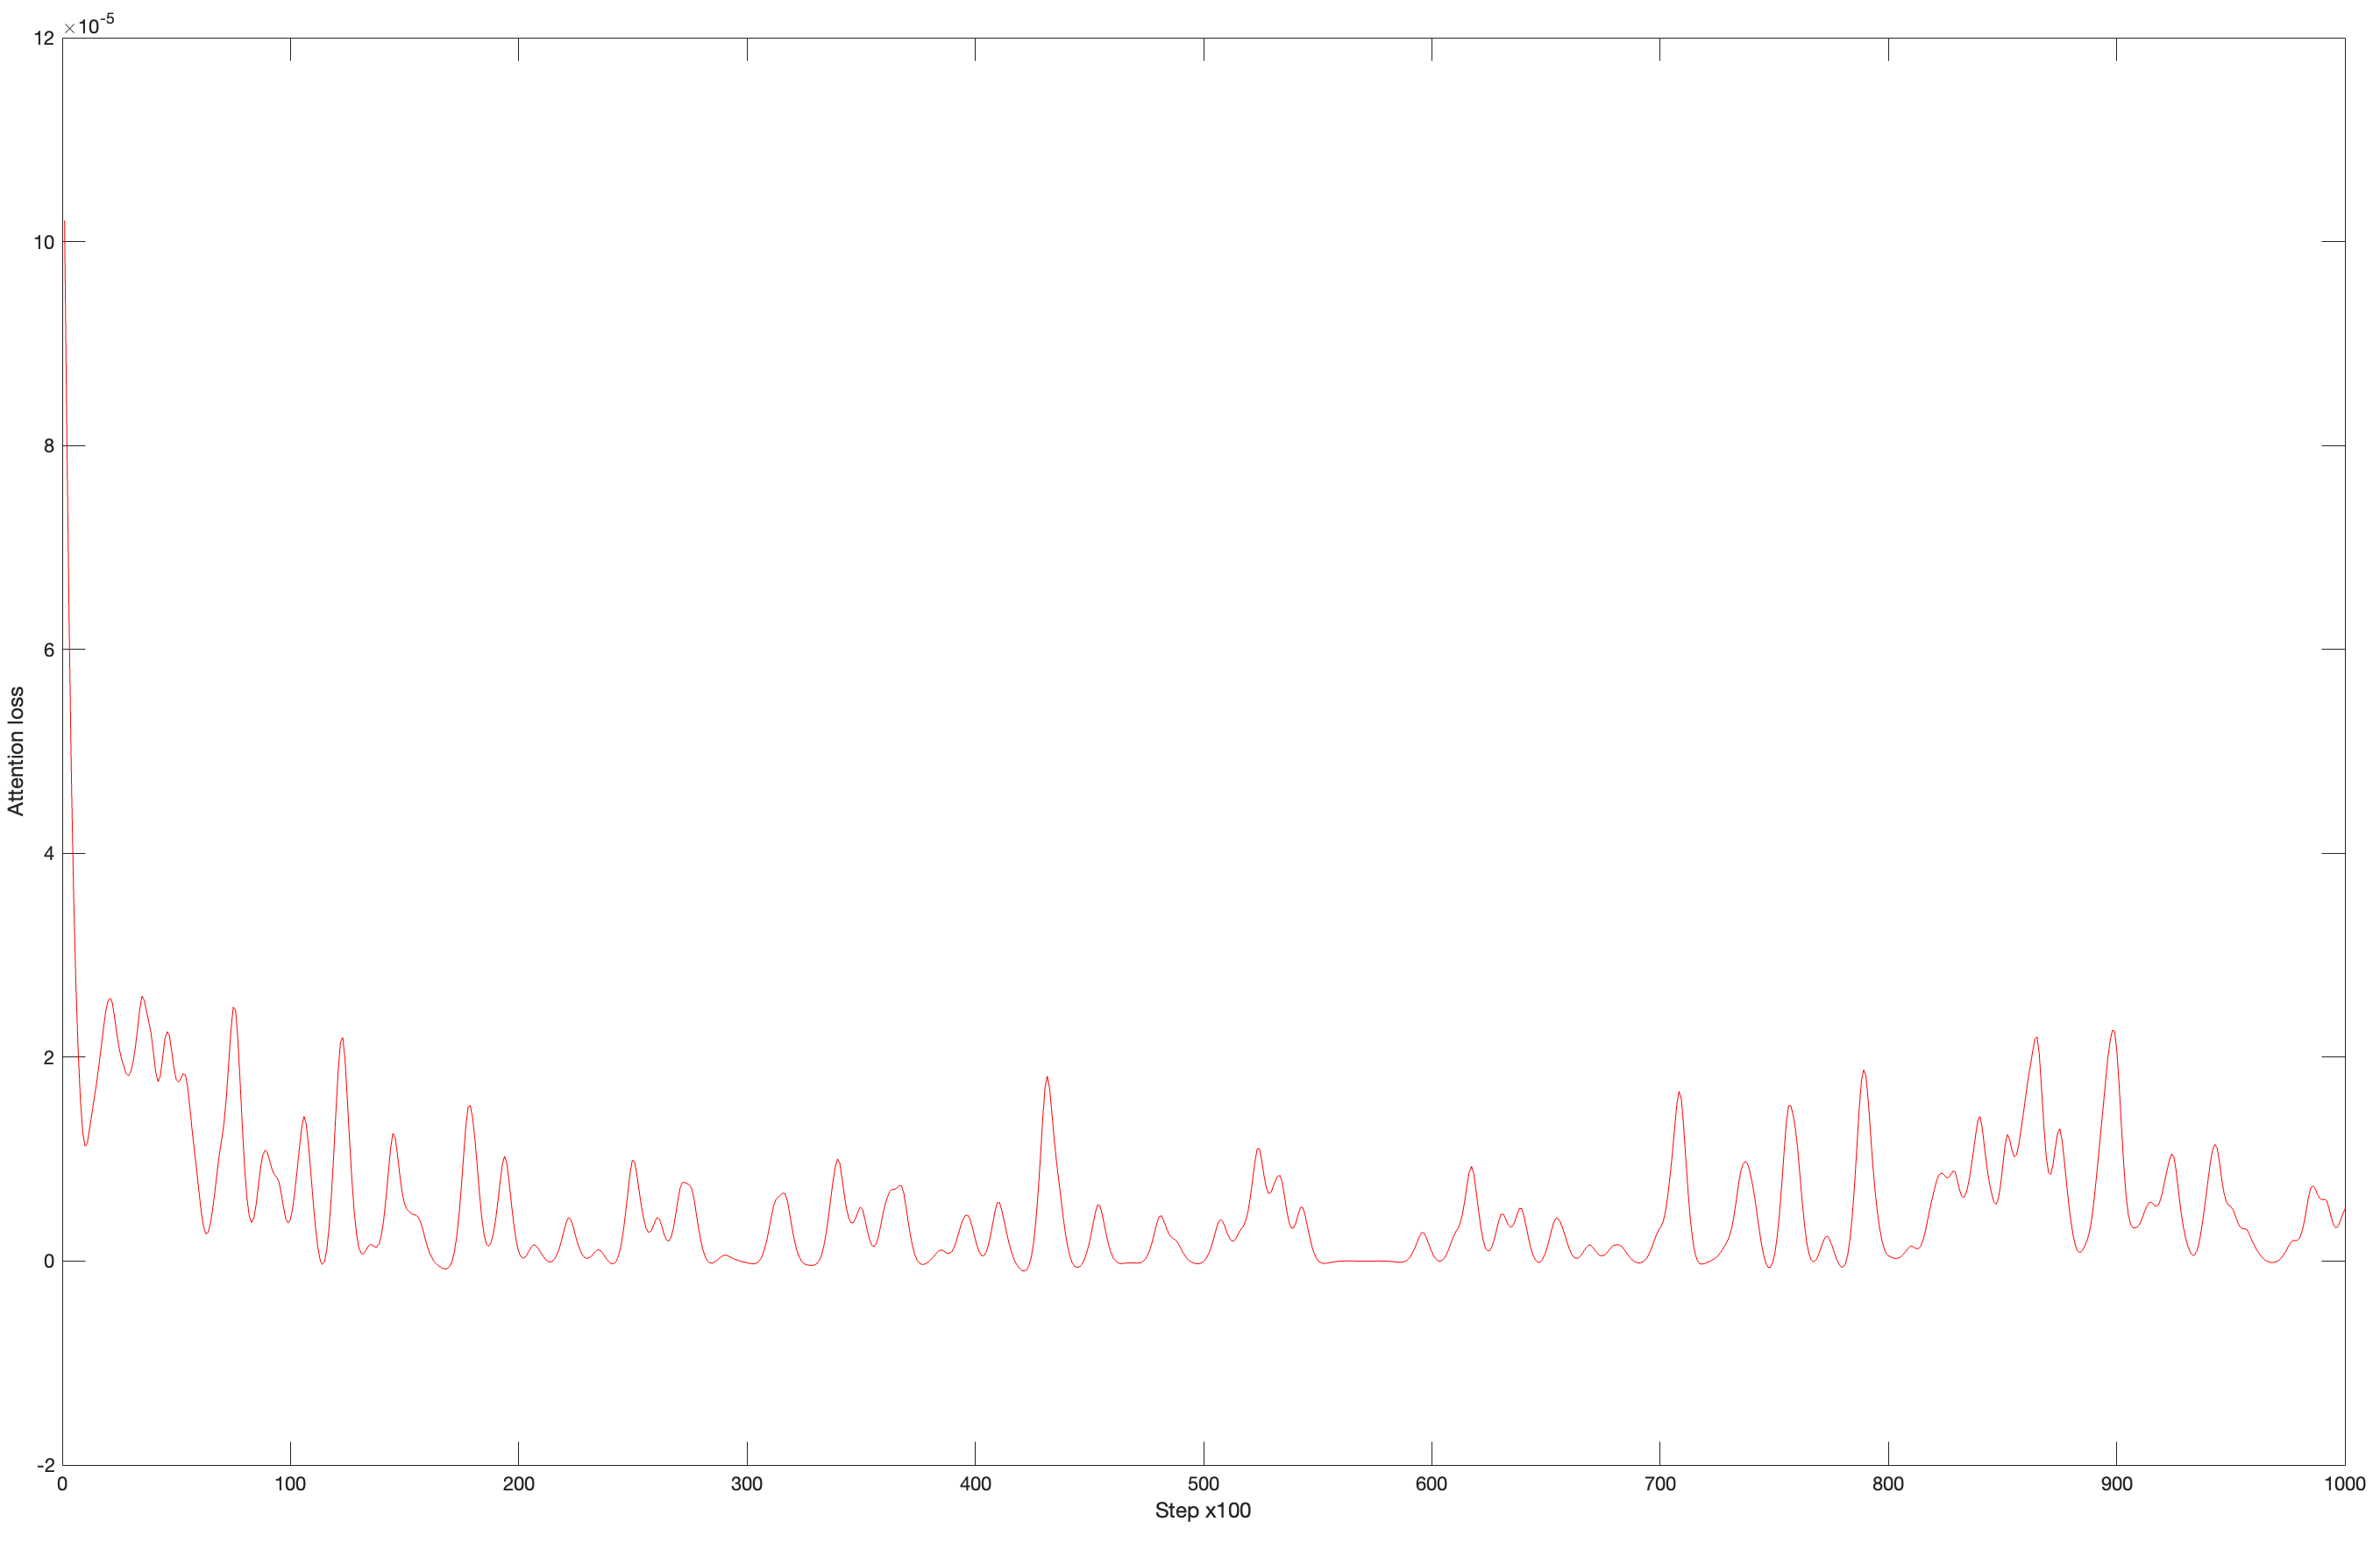
\includegraphics[width=0.9\linewidth]{figures/result/attention_loss}
	\caption[Training result of the Attention Loss]{Training result of the Attention Loss.}
	\label{fig:attention_loss_result}
\end{figure}

In the object decoder in our model in Fig.~\ref{fig:objectdecoder}, we will obtain the corresponding attention map when we get the object feature. Its size is $ 64\times1369 $, corresponding to each object, we draw it into a size of $ 37\times37 $ object attention map. As shown in Fig.~\ref{fig:train_attention_loss} and Fig.~\ref{fig:bus}.We selected the first and second image in our test data set, and drew the object bounding boxes and their attention maps (with and without attention loss).

We can find that our attention has a very good effect on the attention map. Without attention loss, the attention map is messy. As shown in Fig.~\ref{fig:train_attention_loss}(b), we can clearly see the position and shape of the train, and even better express the position of the train than the bounding box. And the area in other parts of the picture is shown in blue, the background is very clean, highlighting the attention weight of our object, making our decoder pay more attention to this object.


\begin{table}[!h]
	\centering
	\begin{tabular}{c|ccc|ccc}
		\bottomrule
		\multirow{2}{*}{}           & \multicolumn{3}{c|}{PredCLS} & \multicolumn{3}{c}{SGCLS} \\ \cline{2-7} 
		& R@20    & R@50    & R@100    & R@20   & R@50   & R@100   \\ \hline
		without our attention  loss & 53.9      & 61.8       & 64.0       & 25.7     & 30.7     & 31.4   \\
		with our attention loss     & 55.4       & 63.3       & 65.2        & 28.4      & 32.7      &33.6     \\ \bottomrule
	\end{tabular}

\caption[The result of attention loss in PredCLS and SGCLS]{The result of attention loss in PredCLS and SGCLS.}
\label{tab:result_attetnion_loss}
\end{table}

According to Table~\ref{tab:result_attetnion_loss}, we can know: our attention loss has got a better object feature. In predcls we have an improvement of about 0.1, and in sgcls our improvement is even greater by about 0.2.

Based on the above results, we get the following conclusions:
\begin{enumerate}
	\item Our attention loss can effectively change the attention map so that it can be well visualized and can show the position and shape of each object.
	\item Our attention loss can get a better object feature, so as to better solve the vrd problem.
\end{enumerate}

\subsection{Experiment on Relation Deocder}
In this section, we conducted experiments on the relation decoder. We designed the relation query. Based on the results of the previous object query, we designed a different relation query, and made our relation context have the spatial information and semantic information of the object.

%In Figure~\ref{fig:relation_d_vis}, we can see that the relationship query we designed has differences between each relationship pair. For example, in the figure (a) represents pair $ <man, pants?>$ and (b) represents pair $ <pant, man> $, their subject and The objects are opposite, but their relations are different. In the figure (c) is relation pair $ <man1, glove> $ and d is $ <man1, man2> $. They have the same subject and different objects, but their relation queries are also significantly different.

In Figure~\ref{fig:relation_attetnion}, We show our context effect through attention between relation and object. When we obtain the relation context through the relation decoder, we also obtain the attention map. Its y-axis represents the relation pair and its x-axis represents the object. We visualize it in the subgraph (c). Our relation pair contains both gt pair and no relation pair. For example, in the picture on the left, we can see that our gt pair $<glass, table> $ has higher attention weight for object \textit{`glass'} and \textit{`table'} than others, it means that this pair pays more attention to these two objects \textit{`glass'} and \textit{`table'}.We also have the same effect for no relation pair. For example, in the attention map on the right,the attention values of the object \textit{ `hair'} and \textit{`glove'} in the pair $<hair, glove> $   is higher than the object \textit{`girl'}.

The Table~\ref{tab:result_relation_decoder} is the result of using the realtion decoder in the predcls task. We can know that our relation decoder is very helpful to solve the VRD problem, and the effect is remarkable.
\begin{table}[!h]
	\centering
	\begin{tabular}{c|ccc}
		\bottomrule
		& R@20    & R@50    & R@100      \\ \hline
		without our relation decoder  loss & 51.1    &58.7      & 61.1    \\
		with our relation decoder     & 55.4       & 63.3       & 65.2       \\ \bottomrule
	\end{tabular}
	
	\caption[The result of our relation decoder in PredCLS]{The result of our relation decoder in PredCLS.}
	\label{tab:result_relation_decoder}
\end{table}

%\begin{figure}[h!]
%	\centering
%	\subfigure[]{
%		\begin{minipage}[t]{3.5cm}
%			\centering
%			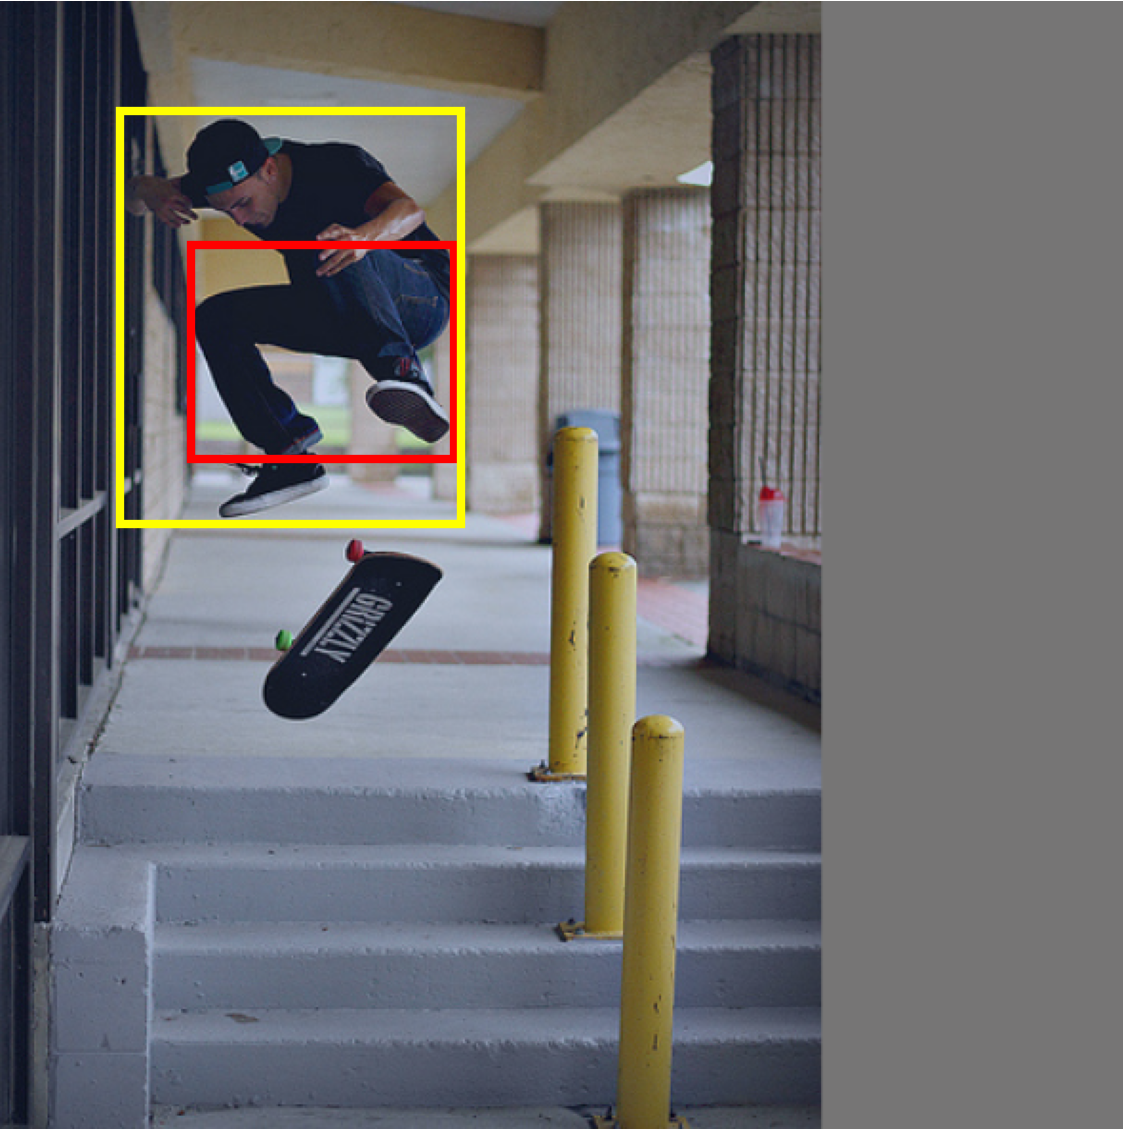
\includegraphics[width=0.9\linewidth]{figures/result/relation/r1}
%	\end{minipage}}
%	\subfigure[]{
%		\begin{minipage}[t]{3.5cm}
%			\centering
%			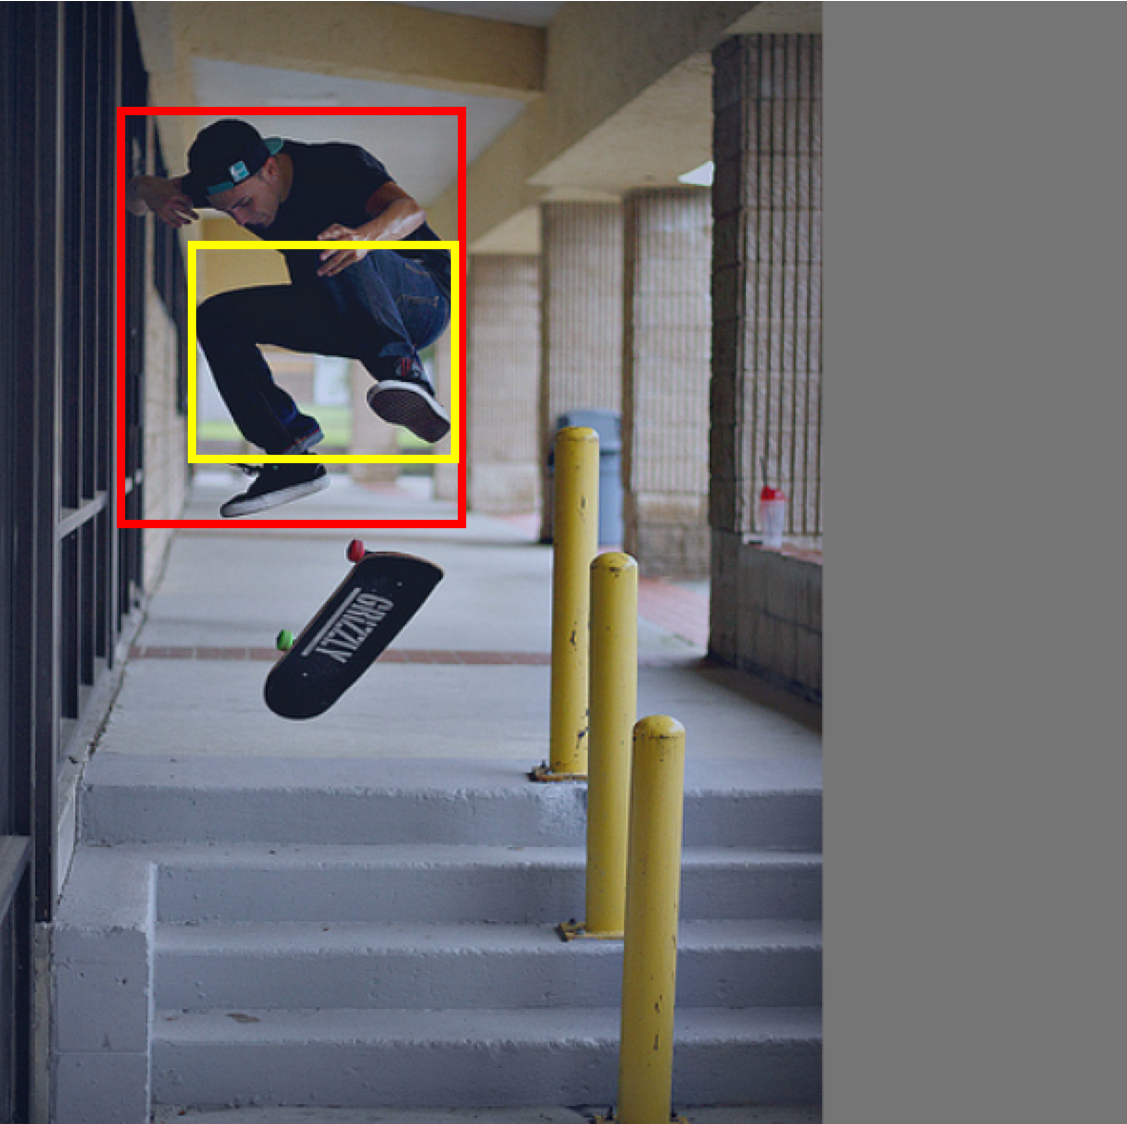
\includegraphics[width=0.9\linewidth]{figures/result/relation/r2}
%	\end{minipage}}
%	\subfigure[]{
%		\begin{minipage}[t]{3.5cm}
%			\centering
%			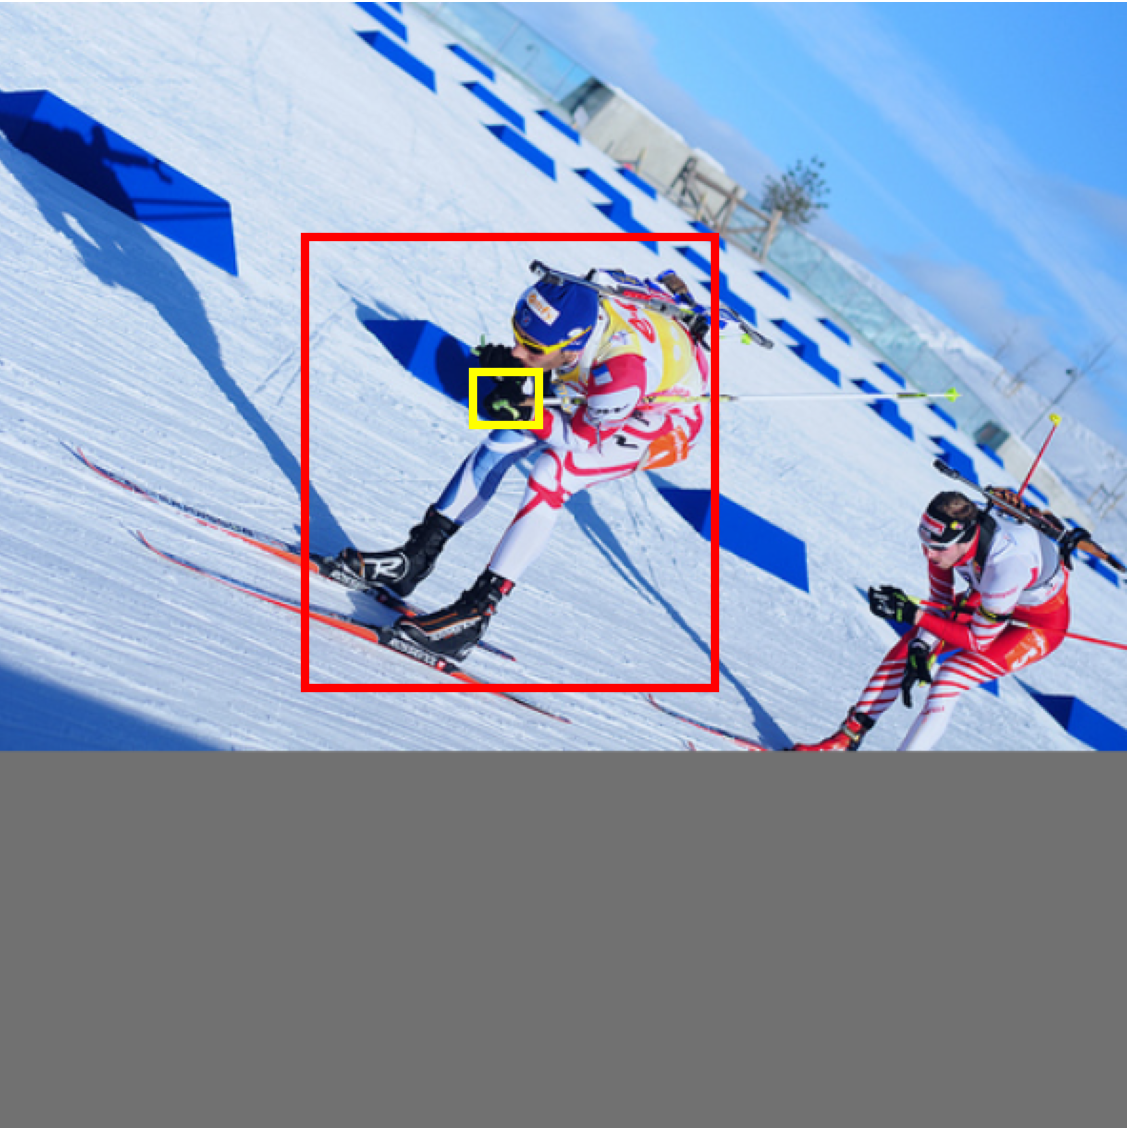
\includegraphics[width=0.9\linewidth]{figures/result/relation/r3}
%	\end{minipage}}
%	\subfigure[]{
%		\begin{minipage}[t]{3.5cm}
%			\centering
%			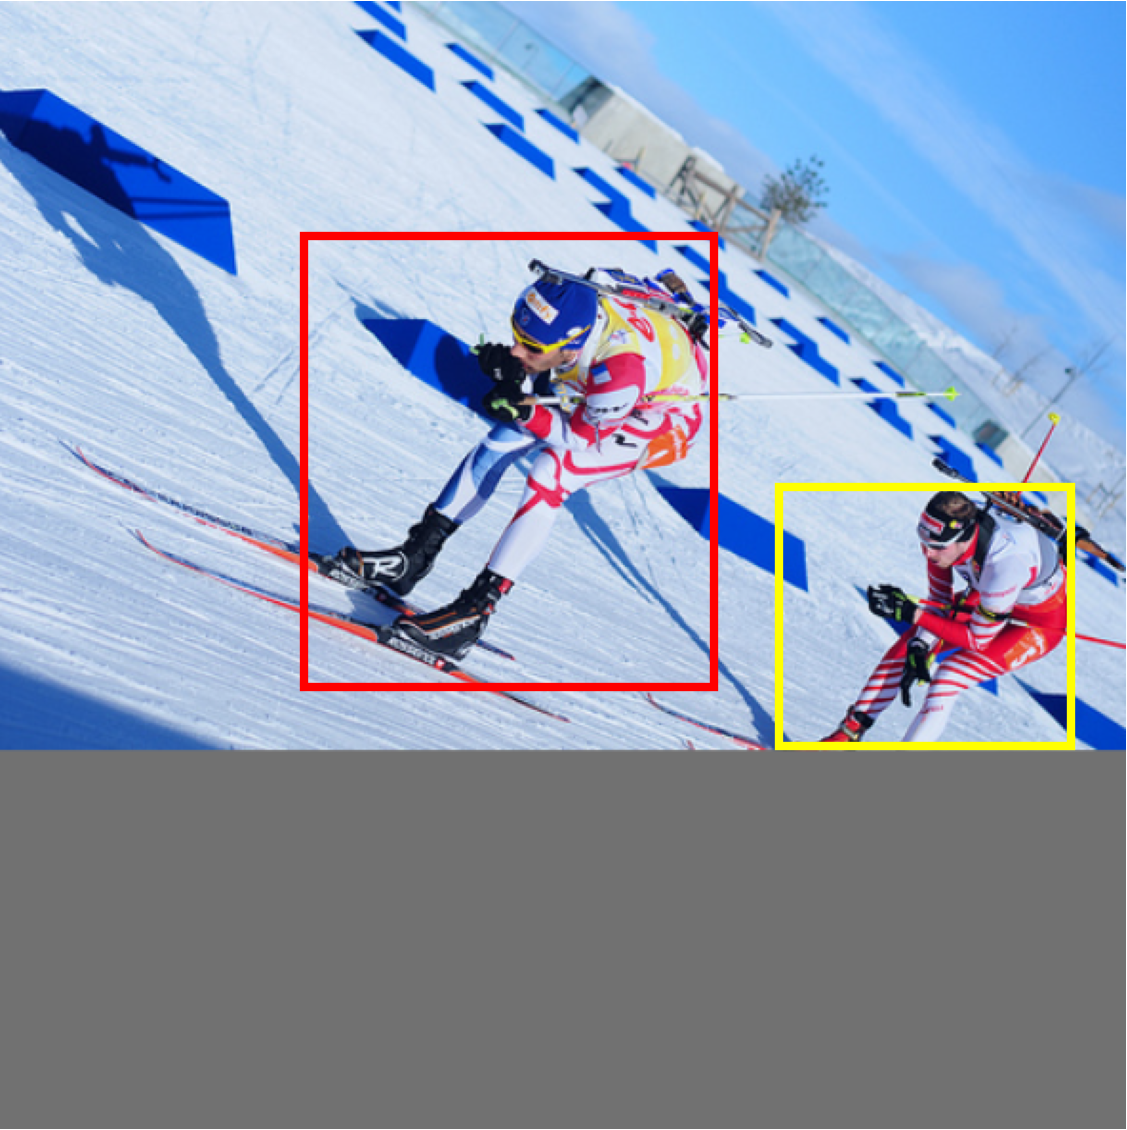
\includegraphics[width=0.9\linewidth]{figures/result/relation/r4}
%	\end{minipage}}
%	
%	\subfigure[]{
%		\begin{minipage}[t]{3.5cm}
%			\centering
%			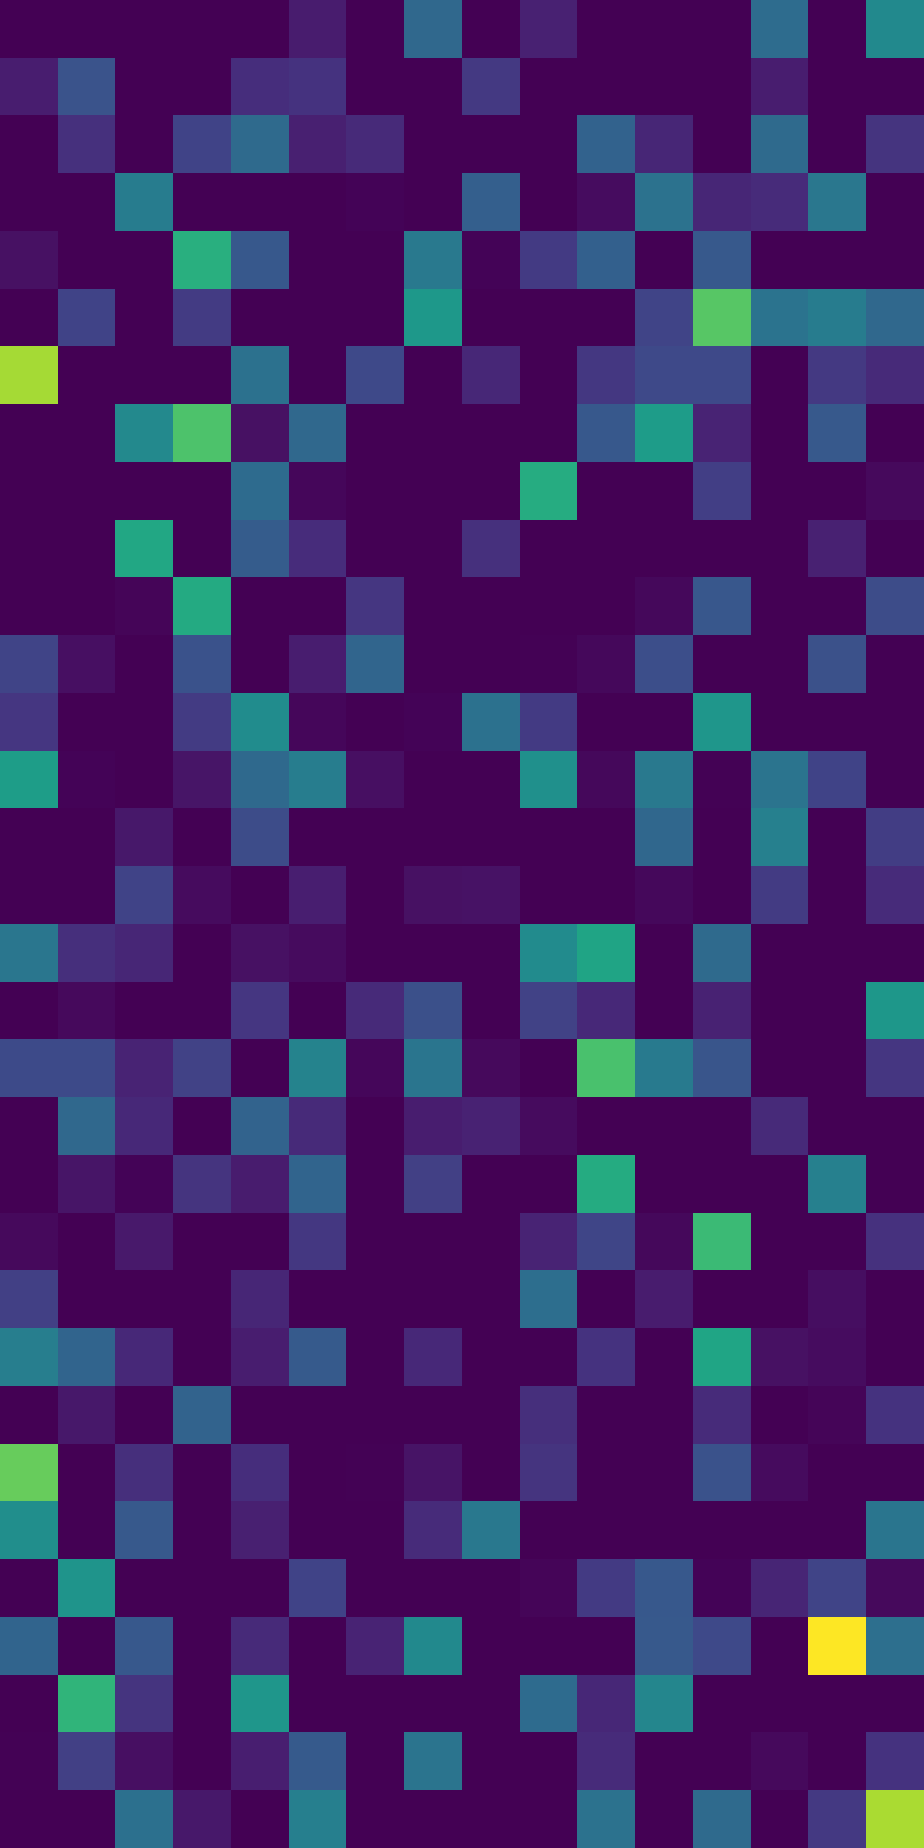
\includegraphics[width=0.9\linewidth]{figures/result/relation/q1}
%	\end{minipage}}
%	\subfigure[]{
%		\begin{minipage}[t]{3.5cm}
%			\centering
%			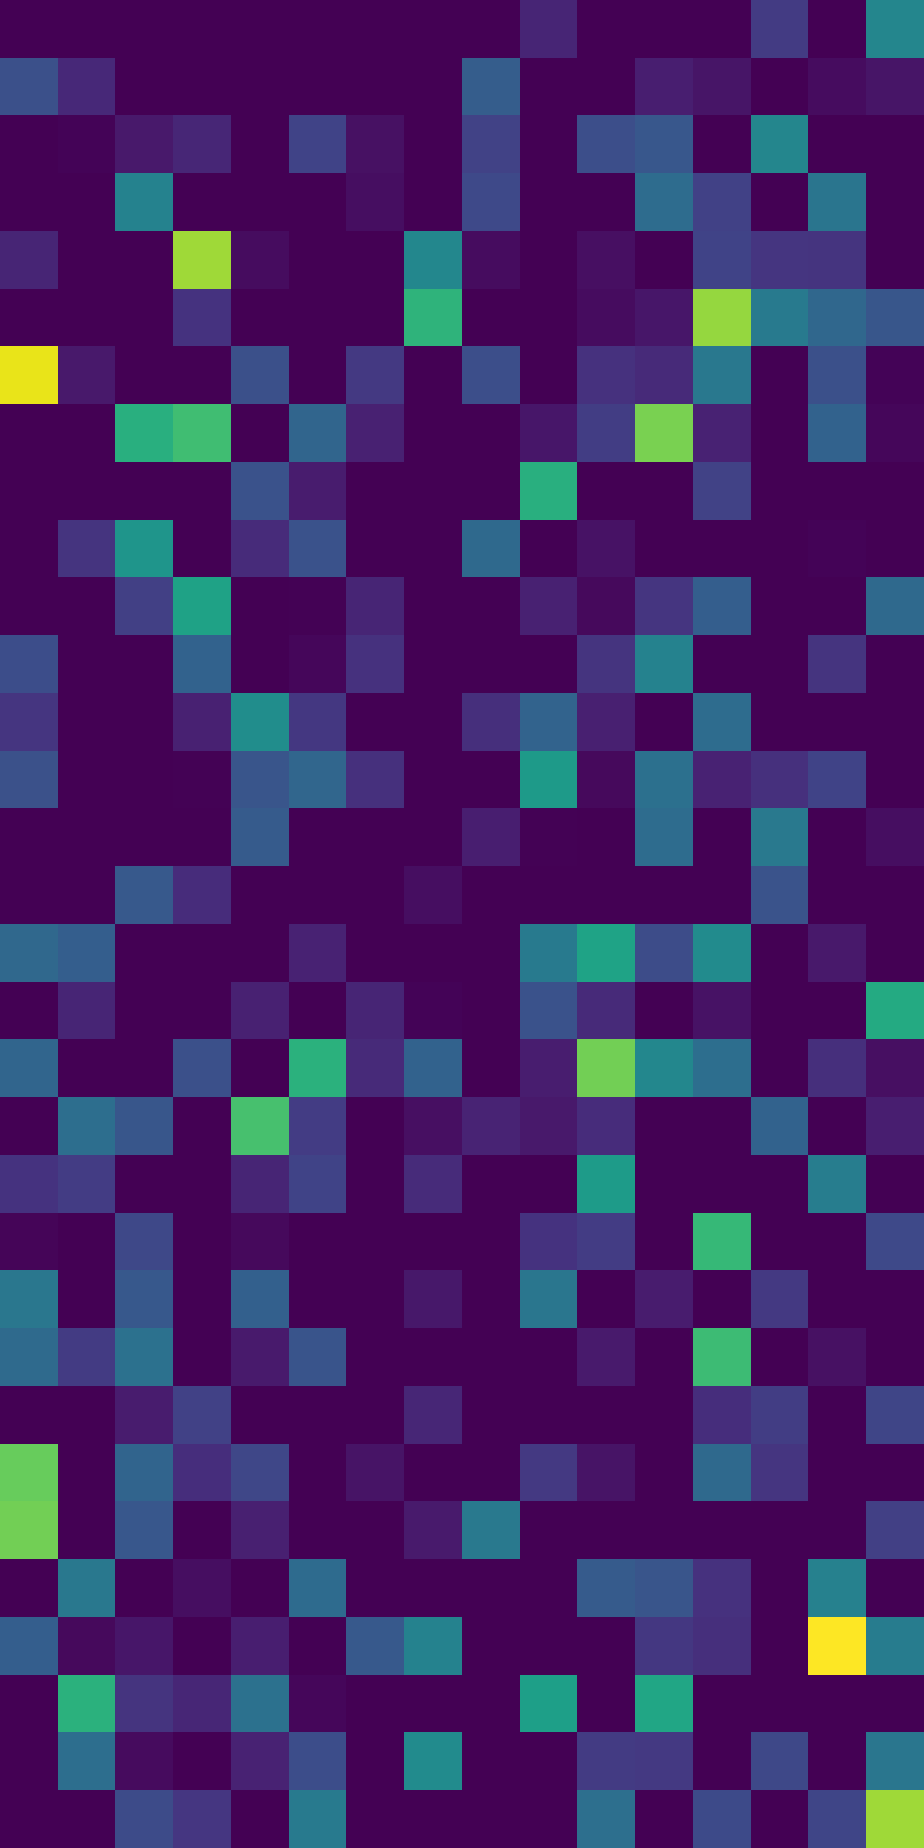
\includegraphics[width=0.9\linewidth]{figures/result/relation/q2}
%	\end{minipage}}
%	\subfigure[]{
%		\begin{minipage}[t]{3.5cm}
%			\centering
%			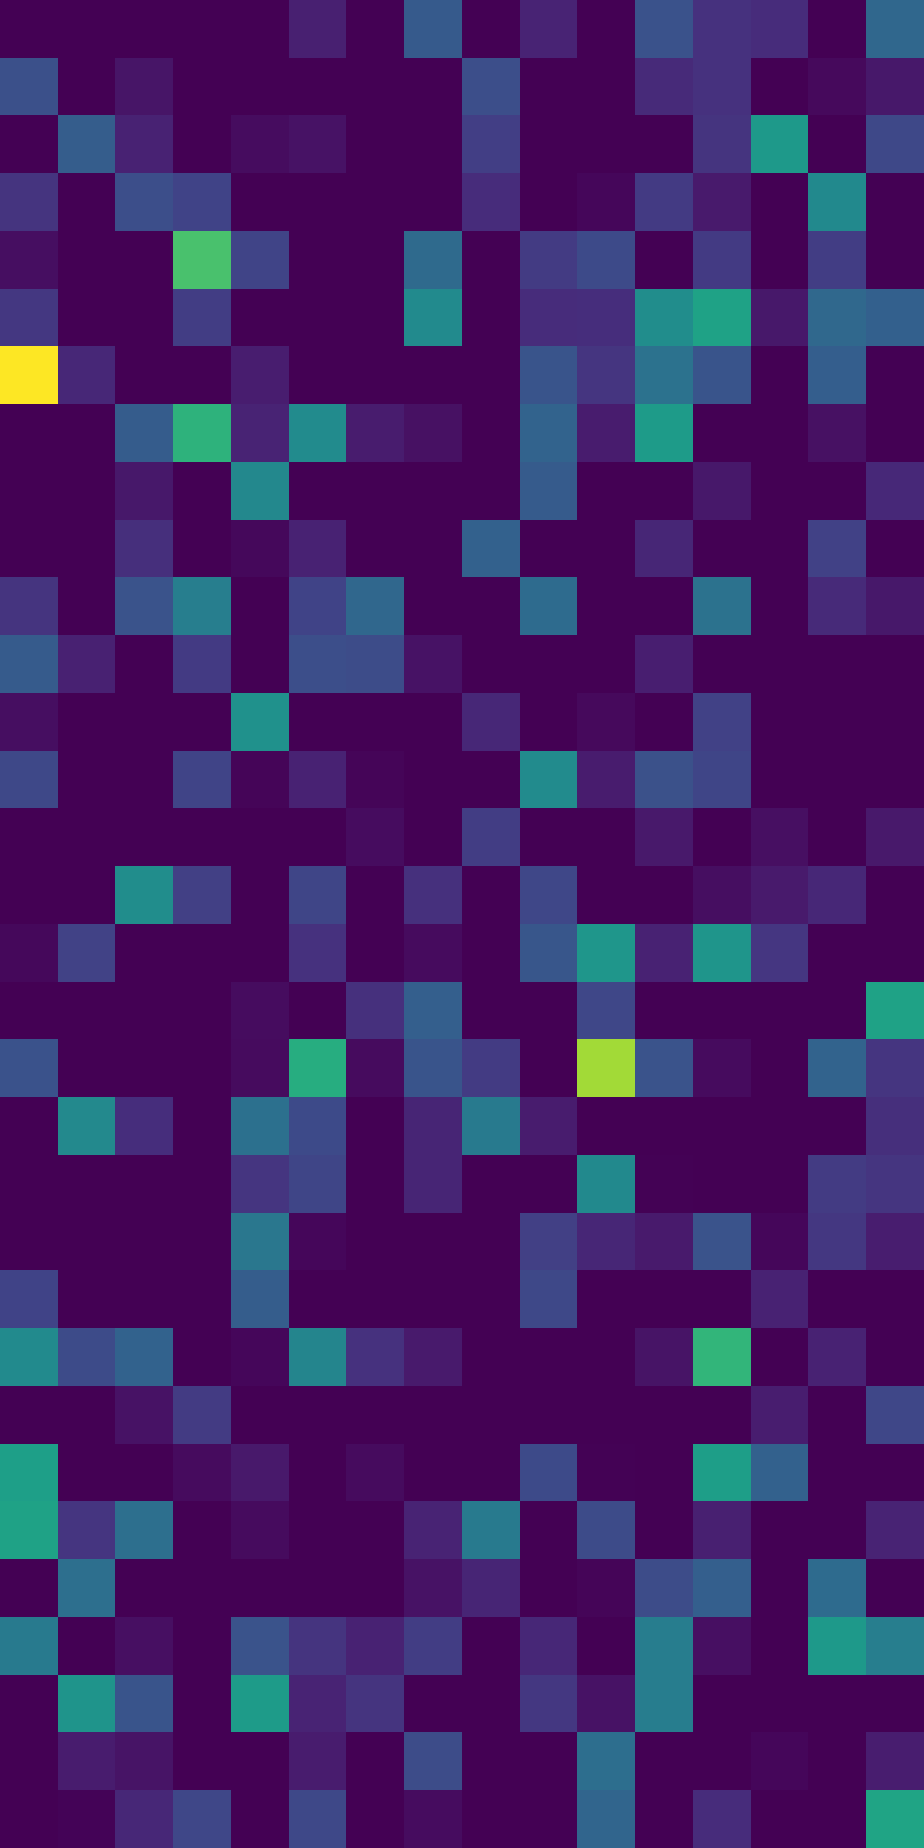
\includegraphics[width=0.9\linewidth]{figures/result/relation/q3}
%	\end{minipage}}
%	\subfigure[]{
%		\begin{minipage}[t]{3.5cm}
%			\centering
%			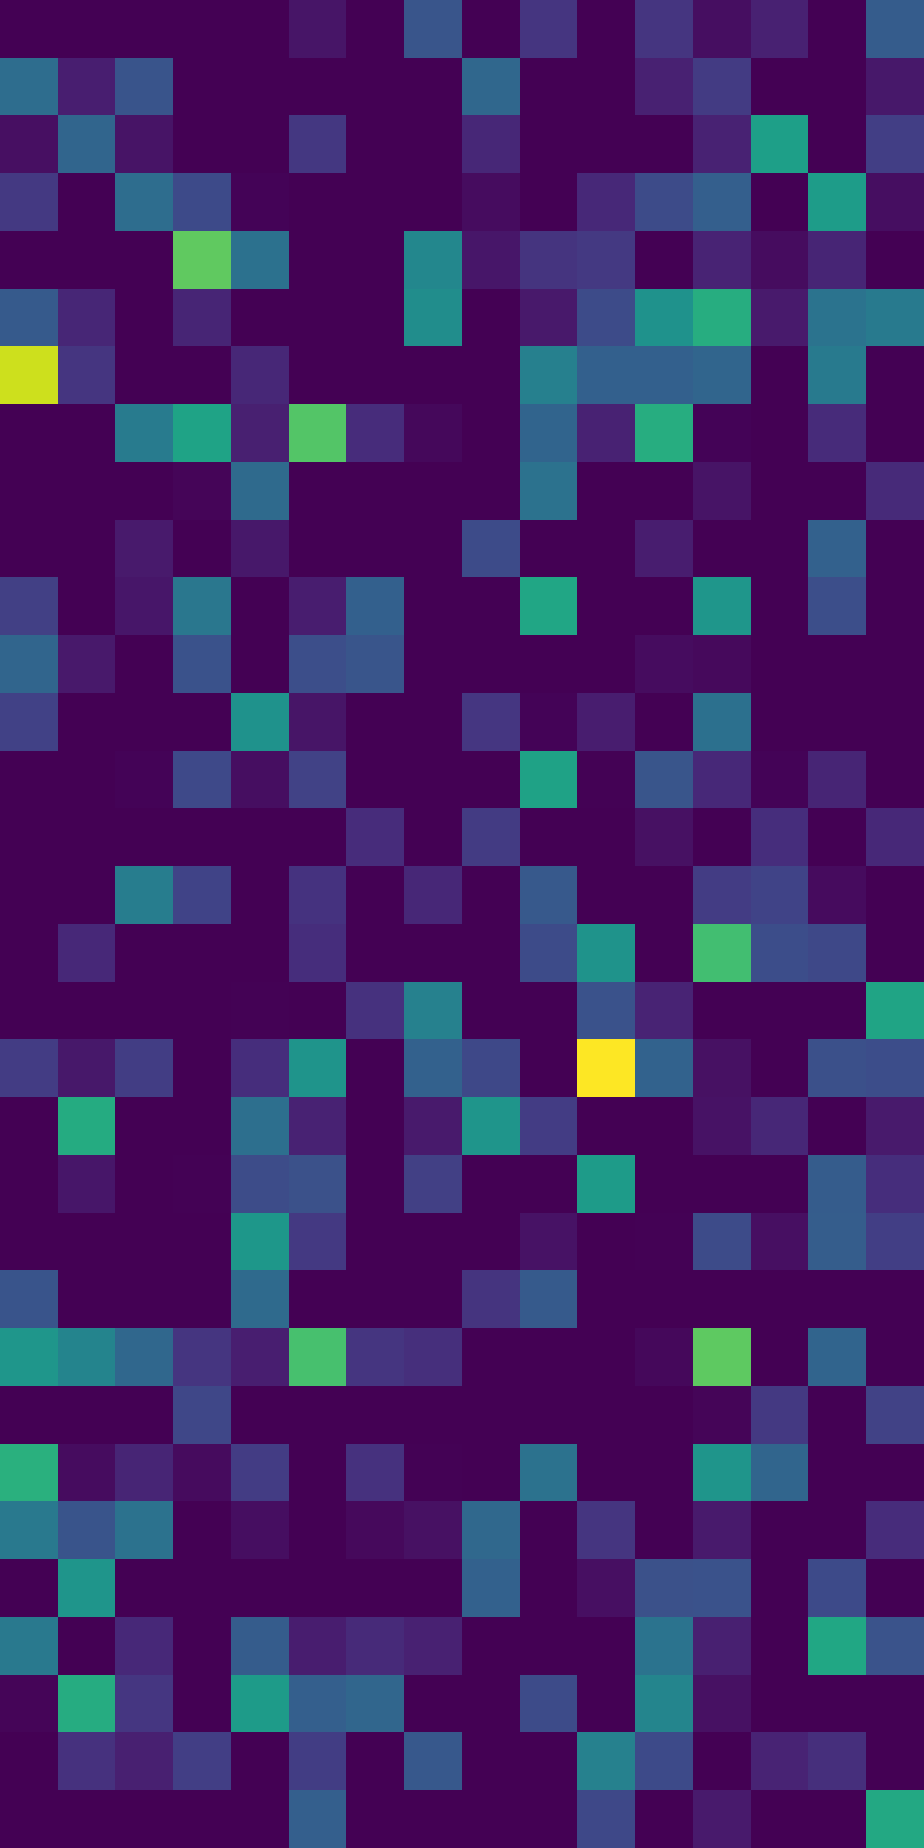
\includegraphics[width=0.9\linewidth]{figures/result/relation/q4}
%	\end{minipage}}
%	
%	\caption[An instance of Visualized results of the relation query]{An instance of visualized results of the object query.from top to bottom, each row represents the position of the object, object query 1, object query 2 and object query 3.}
%	\label{fig:relation_d_vis}
%\end{figure}


\subsection{Results Comparison}
In this section we provide the performance of some advanced related works for comparison in Tab.~\ref{tab:compare_recall}.

\begin{table}[!h]
	\centering
	\resizebox{\textwidth}{16mm}{
	\begin{tabular}{c|ccc|ccc|ccc}
		\hline
		\multirow{2}{*}{Models} & \multicolumn{3}{c|}{PredCLS}                                        & \multicolumn{3}{c|}{SGCLS}                                           & \multicolumn{3}{c}{SGDET}                                          \\ \cline{2-10} 
		& R@20 & R@50 & R@100 & R@20 & R@50 & R@100 & R@20 & R@50 & R@100 \\ \hline
		MESSAGE PASSING~\cite{xu2017scene}         & -                    & 44.8                 & 53.1                  & -                    & 21.7                 & 24.4                  & -                    & 3.4                  & 4.2                   \\
		ASSOC EMBED~\cite{newell2017pixels}             & 47.9                 & 54.1                 & 55.4                  & 18.2                 & 21.8                 & 22.6                  & 6.5                  & 8.1                  & 8.2                   \\
		MSDN ~\cite{li2017scene}                   & -                    & 42.3                 & 48.2                  & -                    & 20.9                 & 24.0                  & -                    & 11.7                 & 14.0                  \\
		FREQ ~\cite{zellers2018neural}                   & 53.6                 & 60.6                 & 62.2                  & 29.3                 & 32.3                 & 32.9                  & 20.1                  & 26.2                 & 30.1                  \\
		MotifNet~\cite{zellers2018neural}                & 58.5                 & 65.2                 & 67.1                  & 32.9                 & 35.8                 & 36.5                  & 21.4                 & 27.2                 & 30.3                  \\
		KERN~\cite{chen2019knowledge}                   & -                    & 65.8                 & 67.6                  & -                    & 36.7                 & 37.4                  & -                    & 27.1                 & 29.8                  \\
		RelDN~\cite{zhang2019graphical}                   & 66.9                 & 68.4                 & 68.4                  & 36.1                 & 36.8                 & 36.8                  & 21.1                 & 28.3                 & 32.7                  \\
		Ours                   & 55.4       & 63.3       & 65.2        & 29.4      & 33.7      &34.6              & 20.2                    & 26.3                    & 29.6                     \\ \hline
	\end{tabular}}

\caption[Comparison with some advanced related works.]{Comparison with some advanced related works.}
\label{tab:compare_recall}
\end{table}

From the above table, we can see that although our model does not reach State of the Arts, it can complete the VRD problem well. Note that the evaluation method of RelDN is different from ours, which causes its Recall@20 to be higher than actual.

\subsection{Visible Results}
In this section, we provide some visible experiment results of our model. There are three instances for respectively PredCLS, SGCLS and SGDET. The results are generated by the model illustrated in Fig.~\ref{fig:my_model}.

In Fig.~\ref{fig:predcls} we present an visible experiment result of PredCLS. We give an image from the VG test set with complex scene information (bounding boxes and classes of each object) to our  model to predicts the interactions between the objects in the image. For this single image, it has 5 relationships in the ground truth and our model predicts 3 relationship correctly. The wrong-predicted relationships are $ <window\ on\ bike >$ and $<seat\ on\ bike>$ and $<bike\ has\ seat>$. The possible reasons are: predicates such as \textit{`on' }and \textit{`has' } are the majority in our data set, so our model predicts them into these. But usually the result is not wrong, it's just not in the ground truth.

In Fig.~\ref{fig:sgcls}  we present an visible experiment result of SGCLS. We give an image from the VG test set with scene information(only bounding boxes) to our  model to classifies the object classes and predicts the interactions between the objects in the image. For this single image it has 3 relationships in the ground truth and one relationship are predicted correctly by our model, the recall@50 is 33.3\%. The reason for the low recall of this picture is that we did not predict \textit{`building'} and \textit{`coat'}. The score of \textit{`building'} is only 0.72\% and the score of \textit{`coat'} is only 3.4\%. In subfigure (a), we can see that the bounding box of \textit{`women'} completely occludes the bounding box of \textit{`building'}, and they almost overlap, so it is difficult for our model to accurately classify the \textit{`building'}correctly.Similarly,
The \textit{`coat'} is also blocked a lot by other objects.
 
In Fig.~\ref{fig:sgdet}  we present an visible experiment result of SGDET. We give only an image from the VG test set without other scene information to our model. The model need to detect the position and class of the bounding boxes for each object and predict the interactions between them. For this single image, we predicted one relationship correctly, and there are 3 ground true relationships. Our recall@50 is 33.3\%.  In subfigure (c), we can find some reasons for low recall. For example, the bounding box of \textit{`lamp' }we detected is much smaller than the ground truth, and the IoU between them is 0.23, which will not be detected. On the contrary, the \textit{`screen' }we detected matches the actual picture. Although we got the seemingly correct relationship of $ <scree\ on \ desk> $, it is not in our ground truth.

\begin{figure}[h!]
	\centering
	\subfigure[Scenes graph with bounding boxes and class labels]{
		\begin{minipage}[t]{8cm}
			\centering
			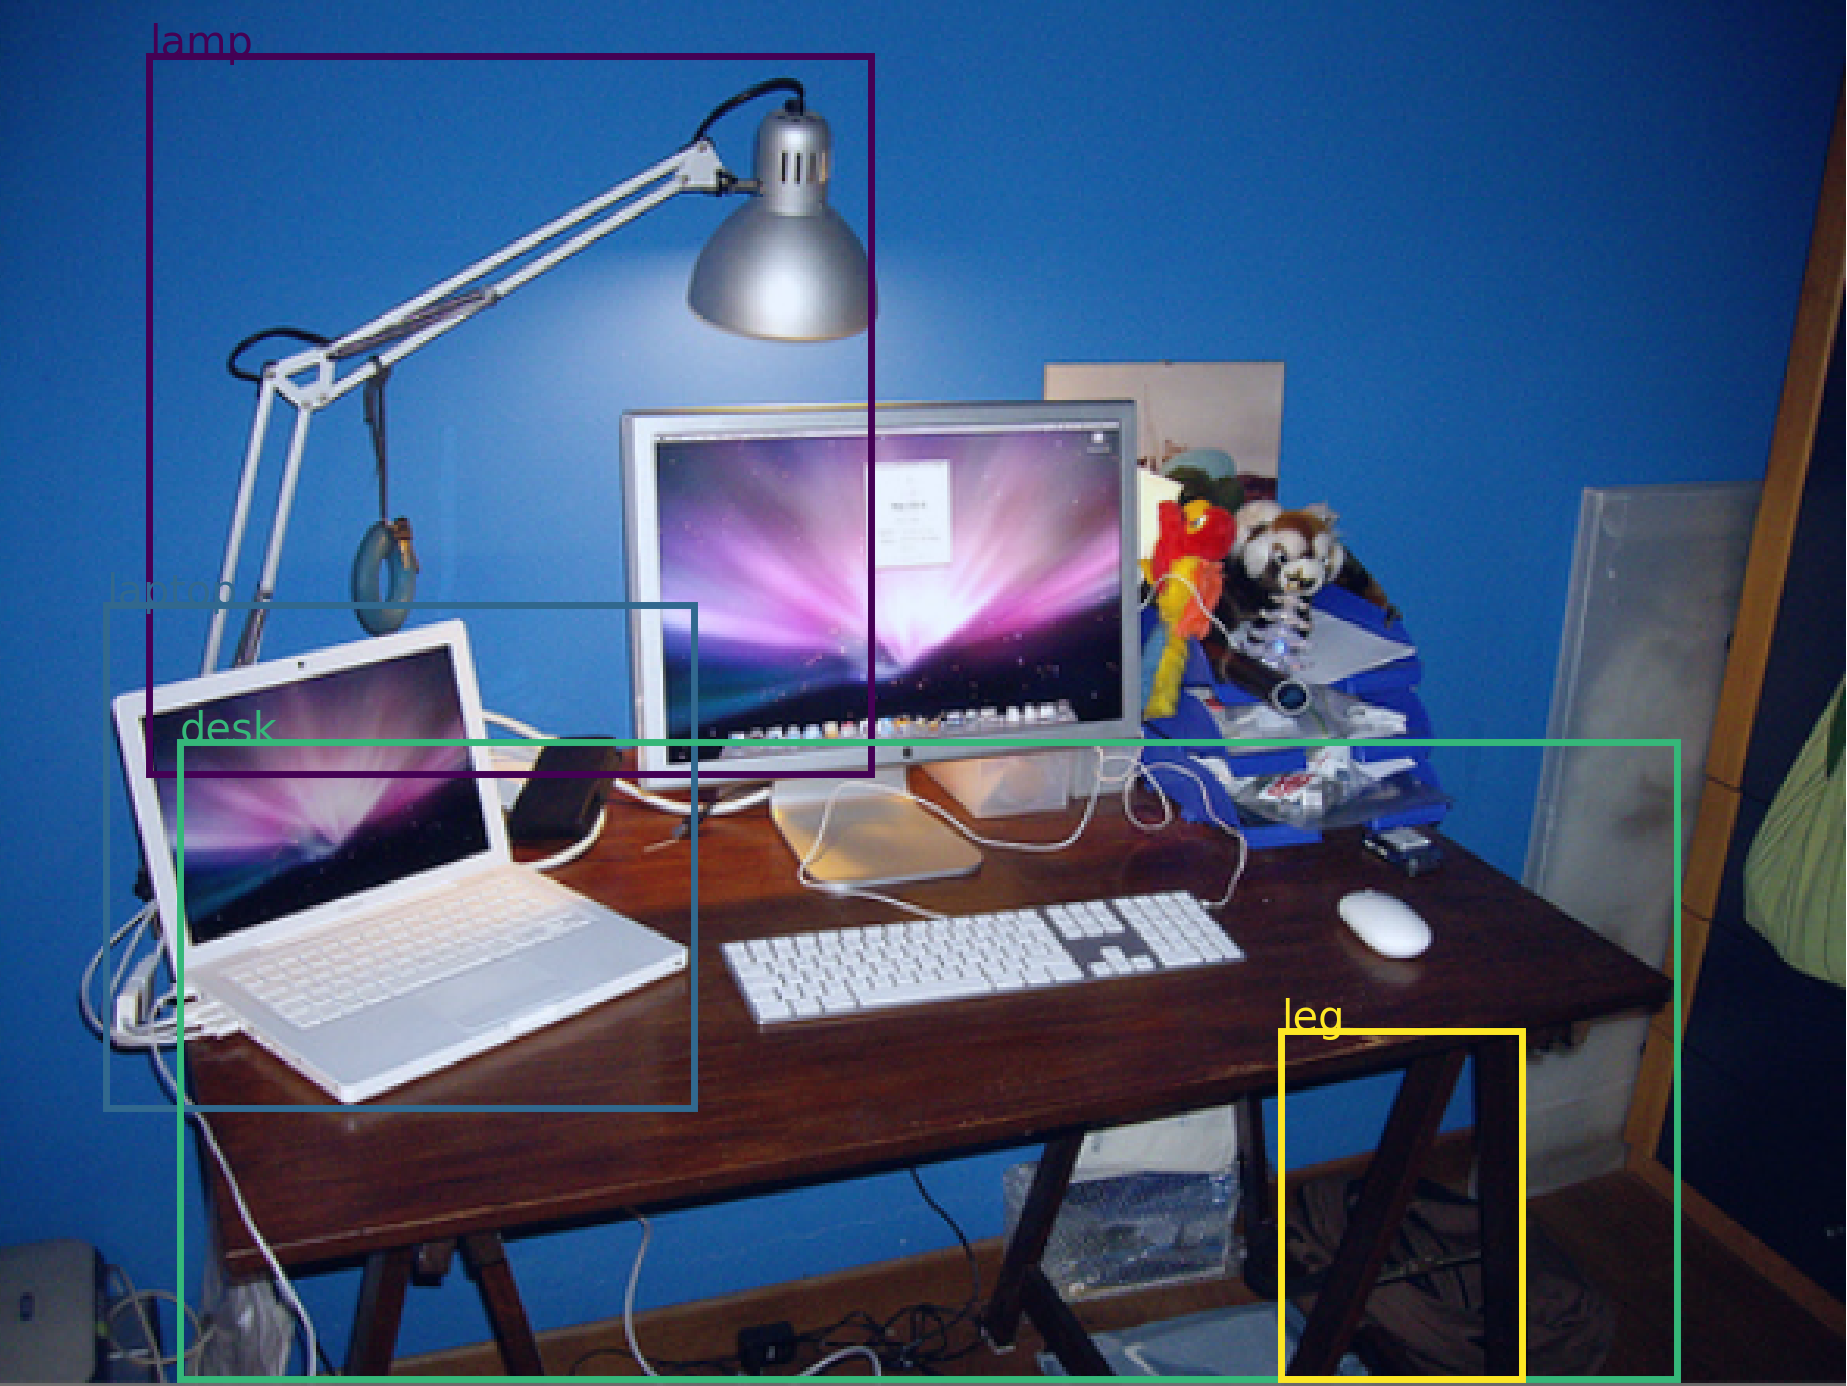
\includegraphics[width=0.95\linewidth]{figures/result/sgdet/img}
	\end{minipage}}
	\subfigure[Grund truth realtion.]{
		\begin{minipage}[t]{6cm}
			\centering
			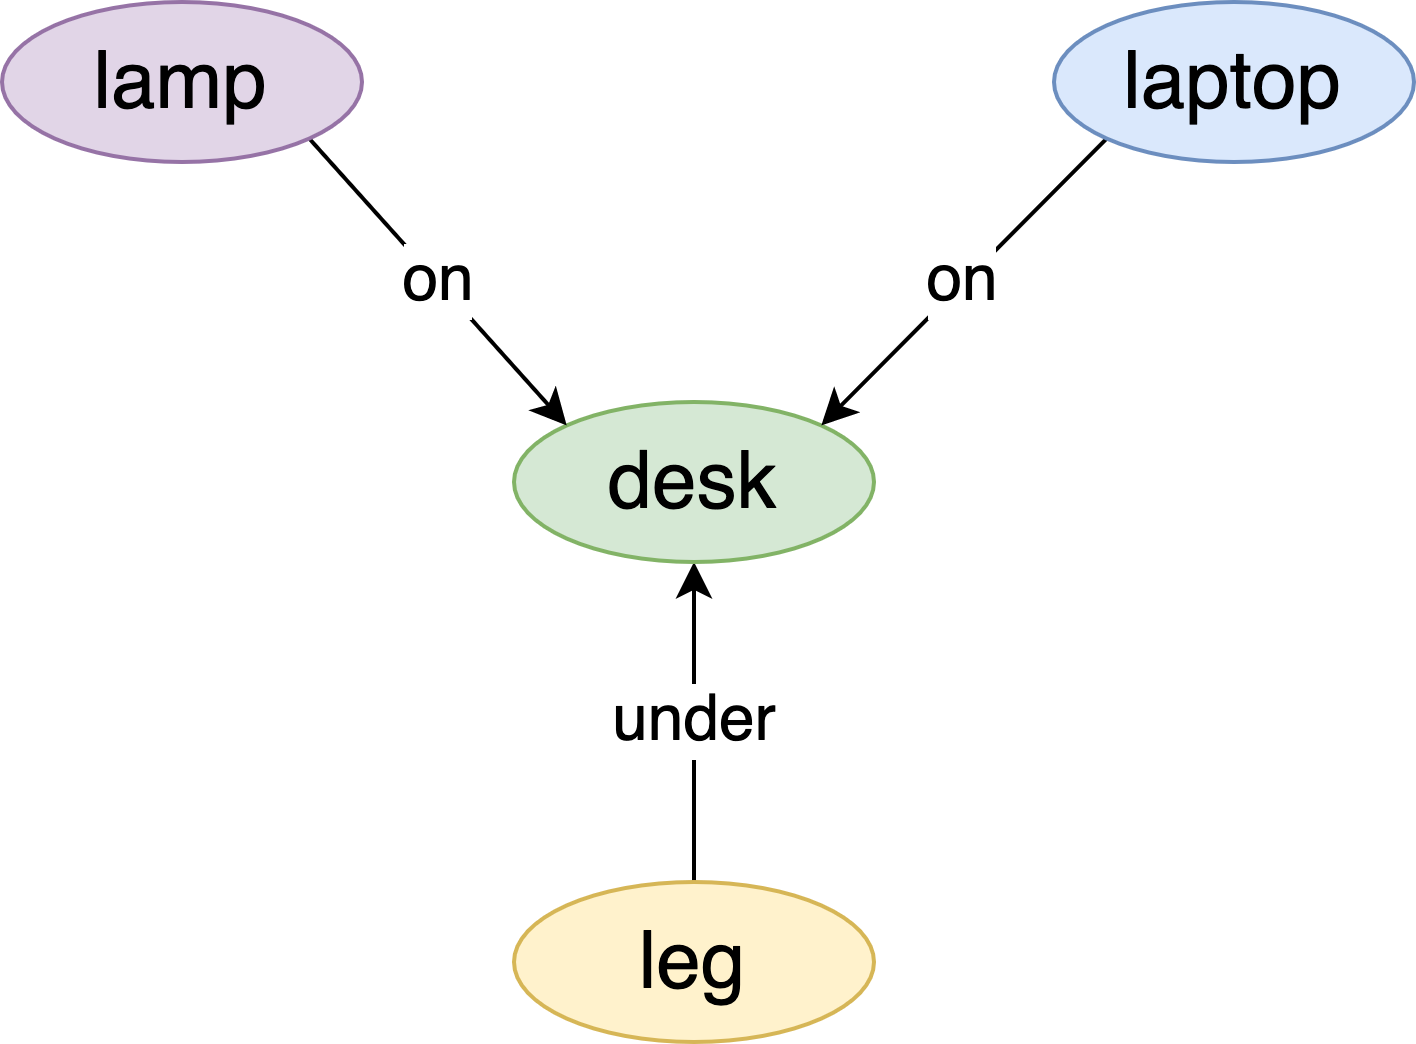
\includegraphics[width=1\linewidth]{figures/result/sgdet/gt}
	\end{minipage}}
	
	\subfigure[Scenes graph with dectected boxes and class labels.]{
		\begin{minipage}[t]{8cm}
			\centering
			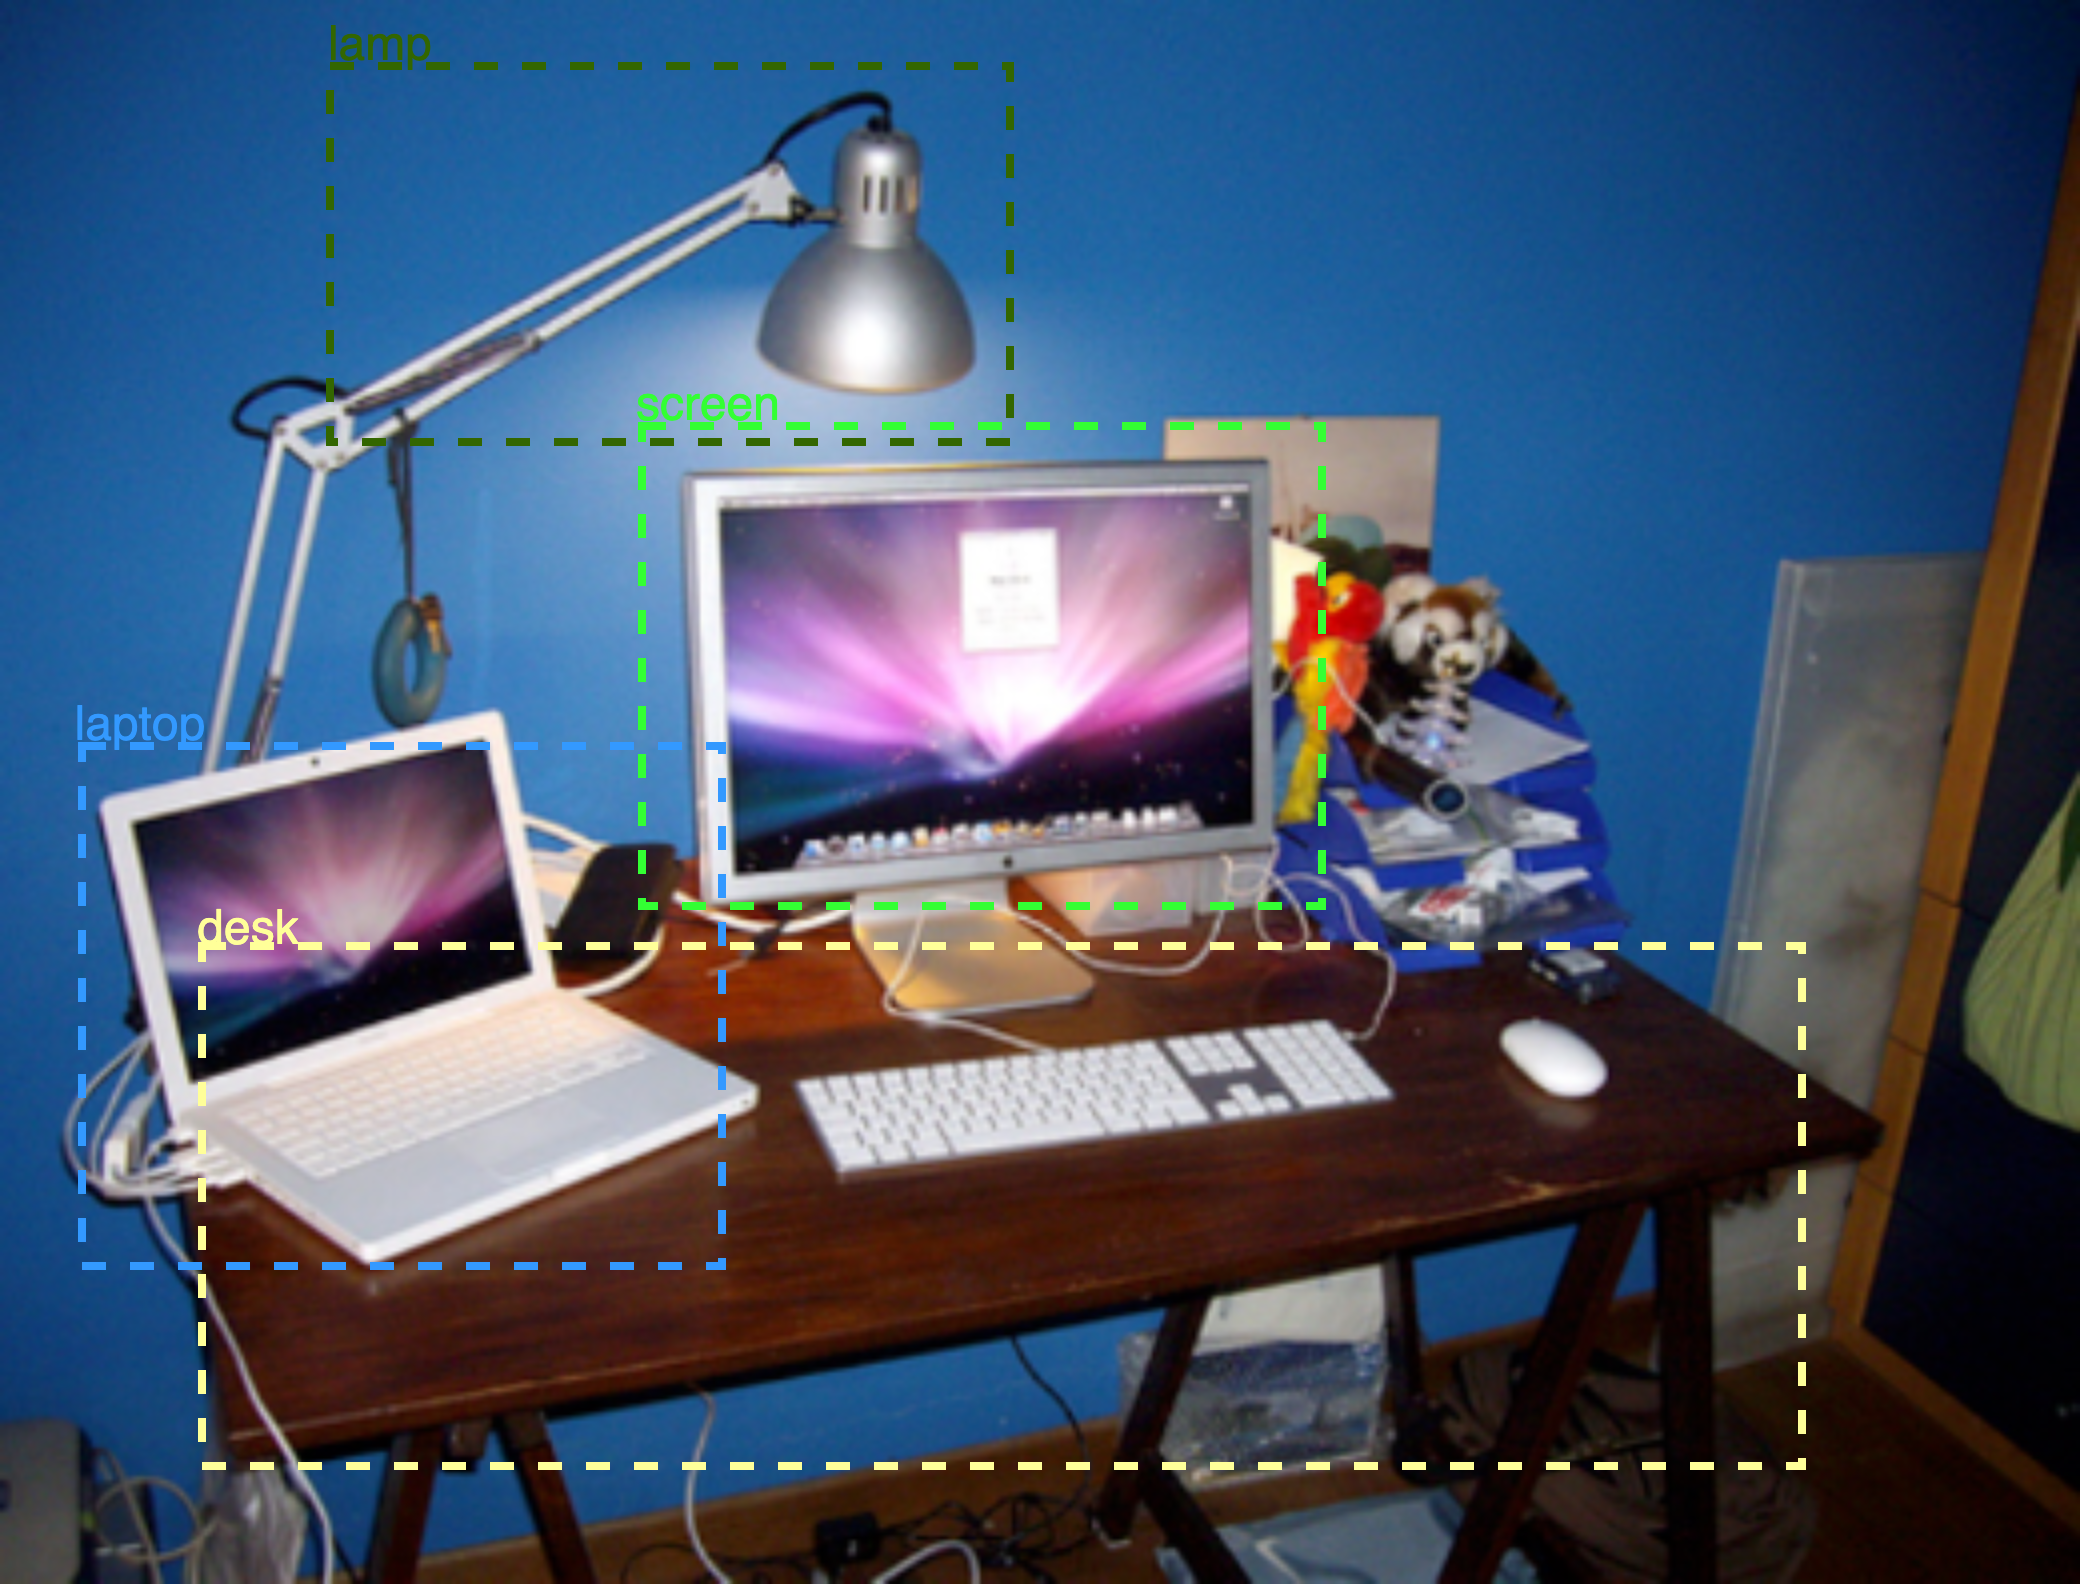
\includegraphics[width=0.95\linewidth]{figures/result/sgdet/img1}
	\end{minipage}}
	\subfigure[The result of Recall@50.]{
		\begin{minipage}[t]{6cm}
			\centering
			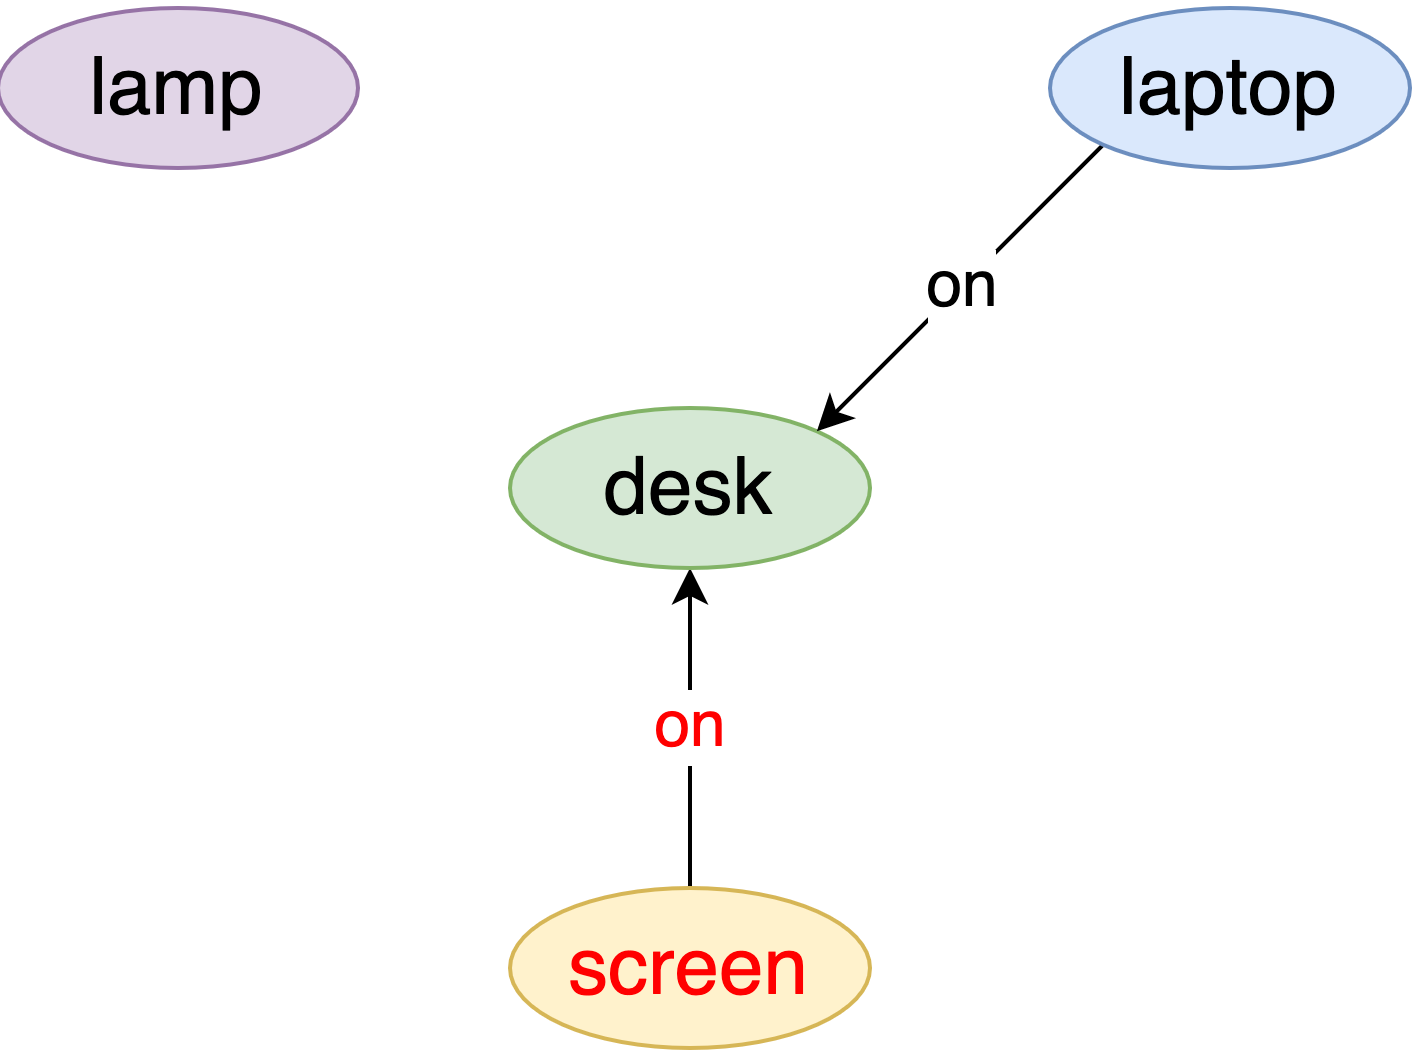
\includegraphics[width=0.9\linewidth]{figures/result/sgdet/rec}
	\end{minipage}}
	
	
	\caption[An instance of SGDET.]{An instance of SGDET.}
	\label{fig:sgdet}
\end{figure}

\begin{figure}[h!]
	\centering
	\subfigure[Scenes graph with bounding boxes and class labels]{
		\begin{minipage}[t]{10cm}
			\centering
			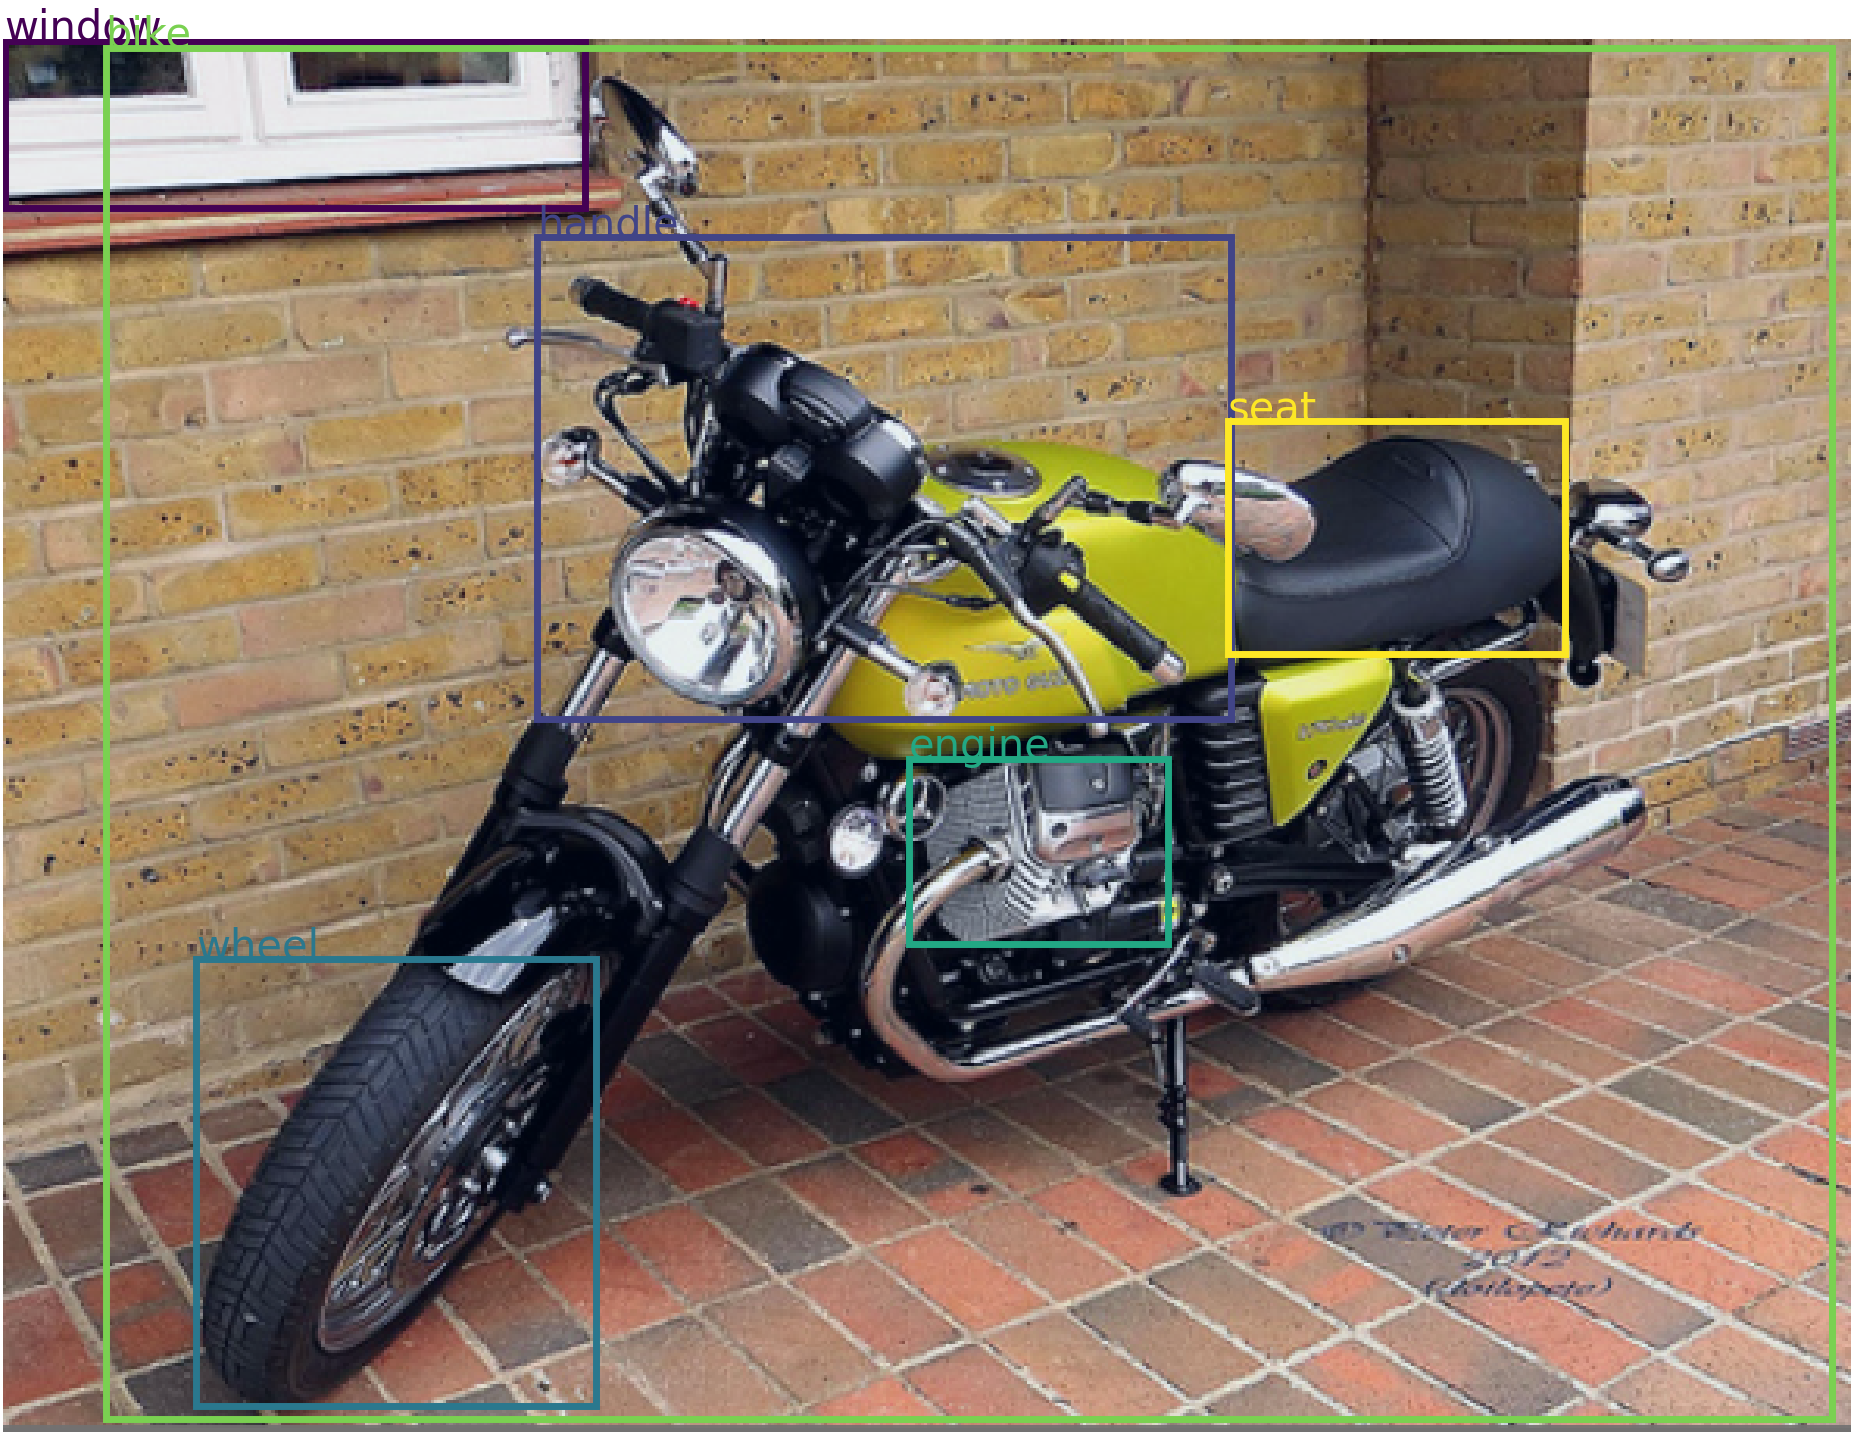
\includegraphics[width=0.8\linewidth]{figures/result/predcls/img}
		\end{minipage}}
	\subfigure[The grund truth realtion.]{
		\begin{minipage}[t]{7cm}
			\centering
			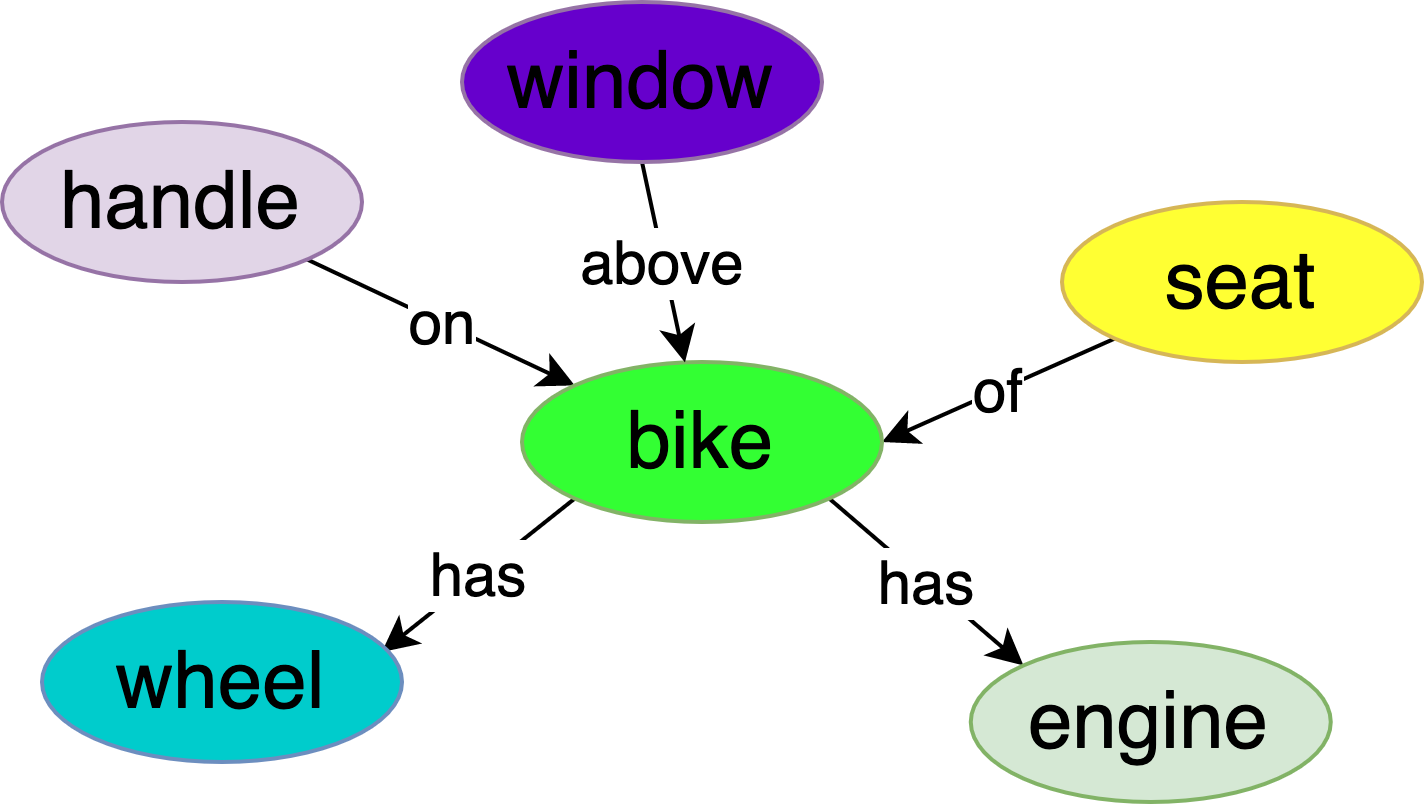
\includegraphics[width=0.8\linewidth]{figures/result/predcls/gt}
		\end{minipage}}
	\subfigure[The result of Recall@50.]{
		\begin{minipage}[t]{7cm}
			\centering
			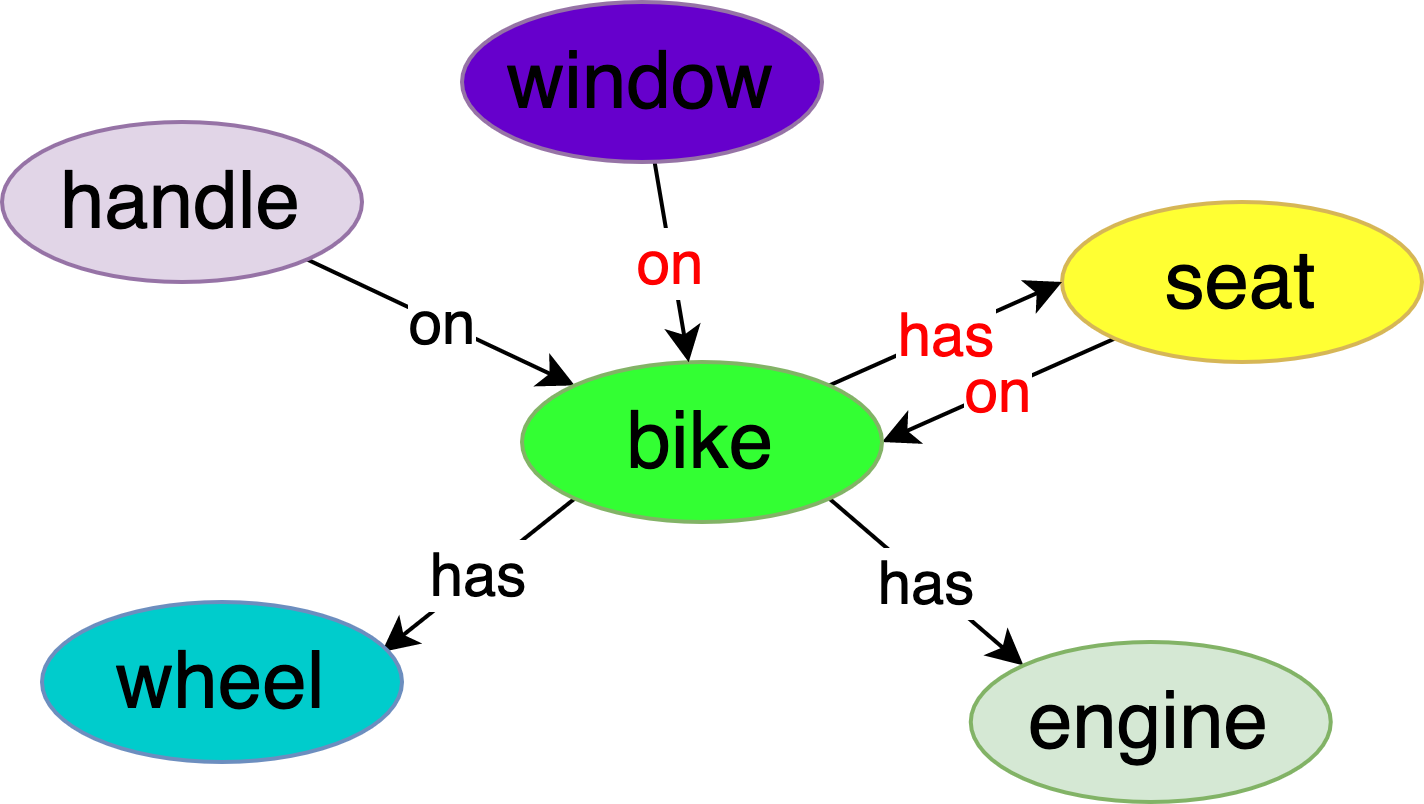
\includegraphics[width=0.8\linewidth]{figures/result/predcls/rec}
	\end{minipage}}
	
	\caption[An instance of PredCLS]{An instance of PredCLS.}
	\label{fig:predcls}
\end{figure}

\begin{figure}[h!]
	\centering
	\subfigure[Scenes graph with bounding boxes and class labels]{
		\begin{minipage}[t]{6cm}
			\centering
			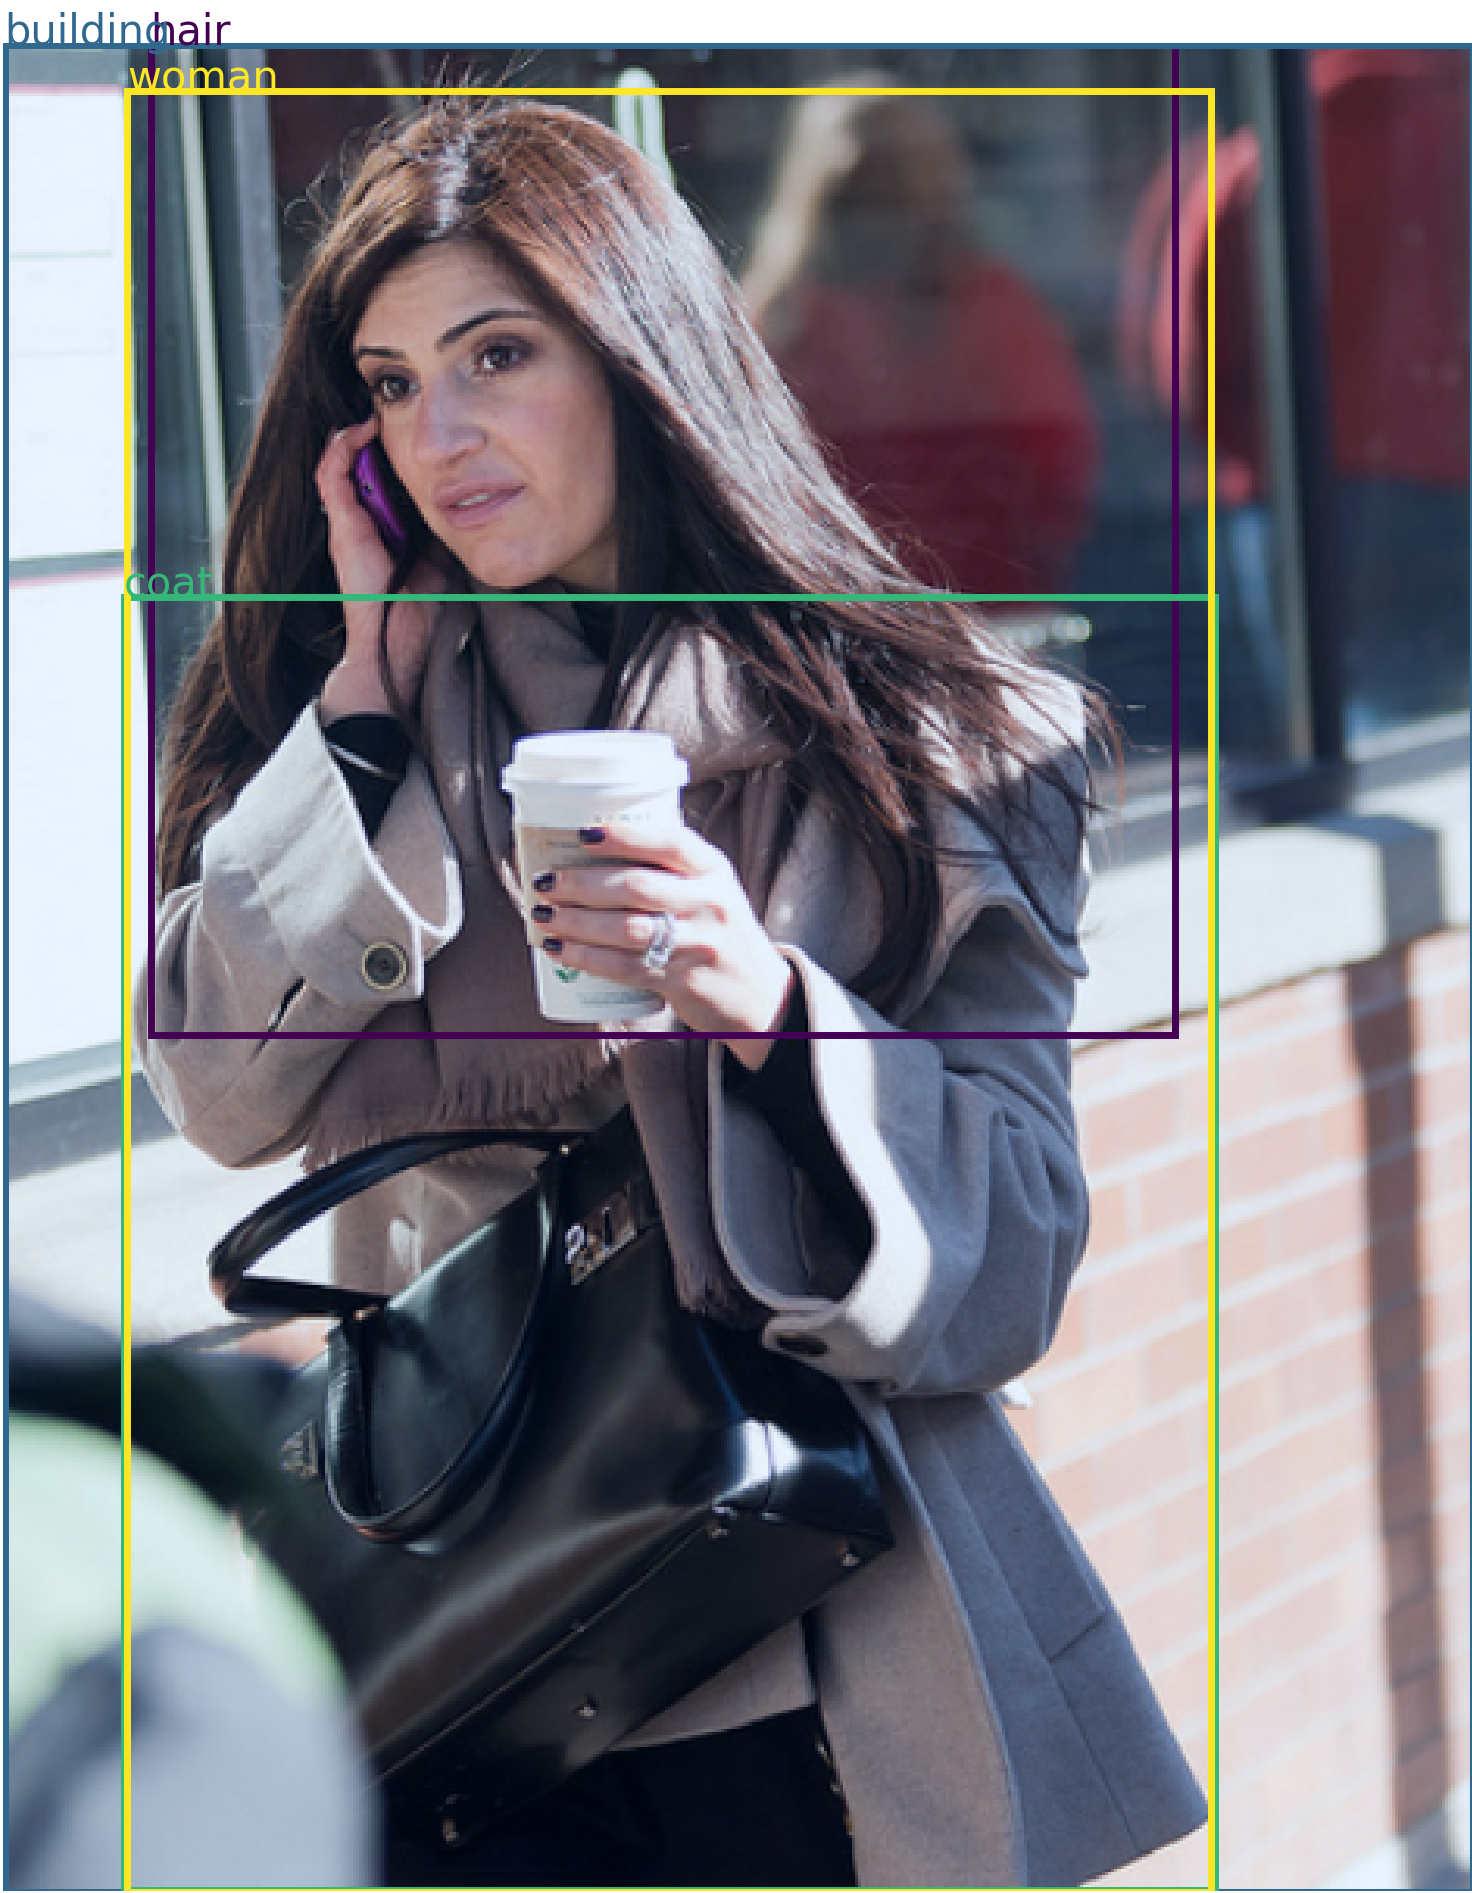
\includegraphics[width=1\linewidth]{figures/result/sgcls/img}
	\end{minipage}}
	\subfigure[Grund truth realtion.]{
		\begin{minipage}[t]{4.5cm}
			\centering
			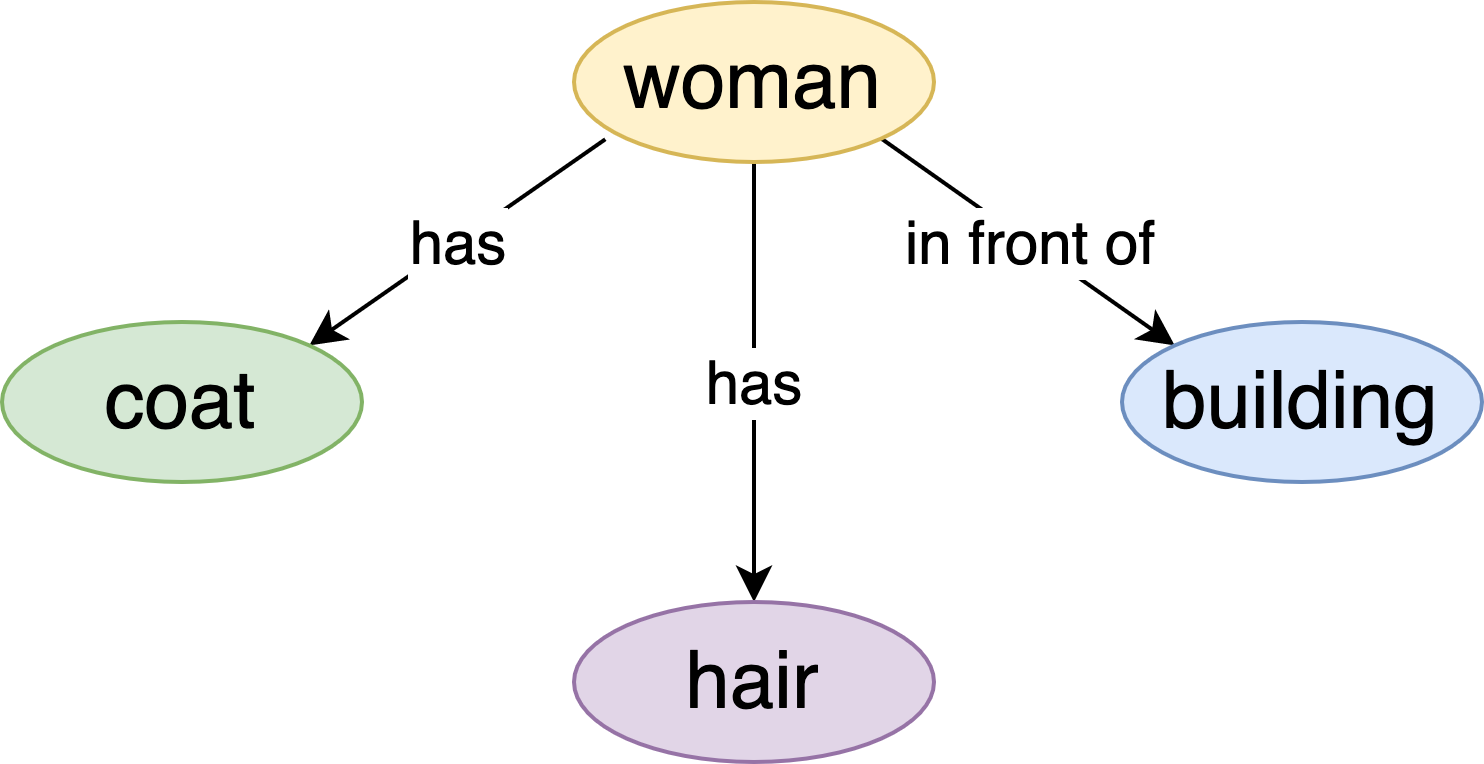
\includegraphics[width=1\linewidth]{figures/result/sgcls/gt}
	\end{minipage}}
	\subfigure[The result of Recall@50.]{
		\begin{minipage}[t]{4.55cm}
			\centering
			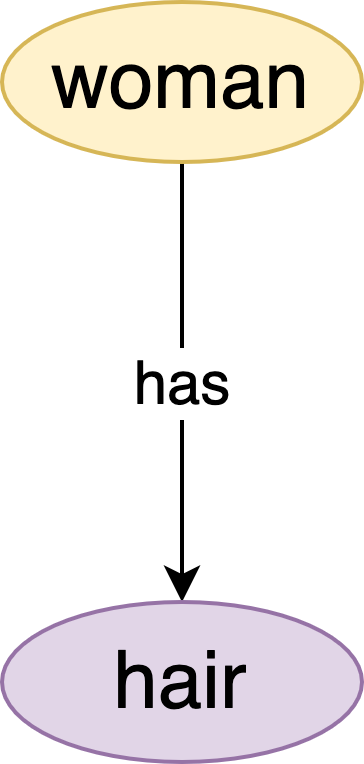
\includegraphics[width=0.3\linewidth]{figures/result/sgcls/rec}
	\end{minipage}}
	
	
	\caption[An instance of SGCLS]{An instance of SGCLS.}
	\label{fig:sgcls}
\end{figure}


\begin{figure}[h!]
	\centering
	\subfigure[Scenes with objects and bounding boxes with class labels]{
		\begin{minipage}[t]{6cm}
			\centering
			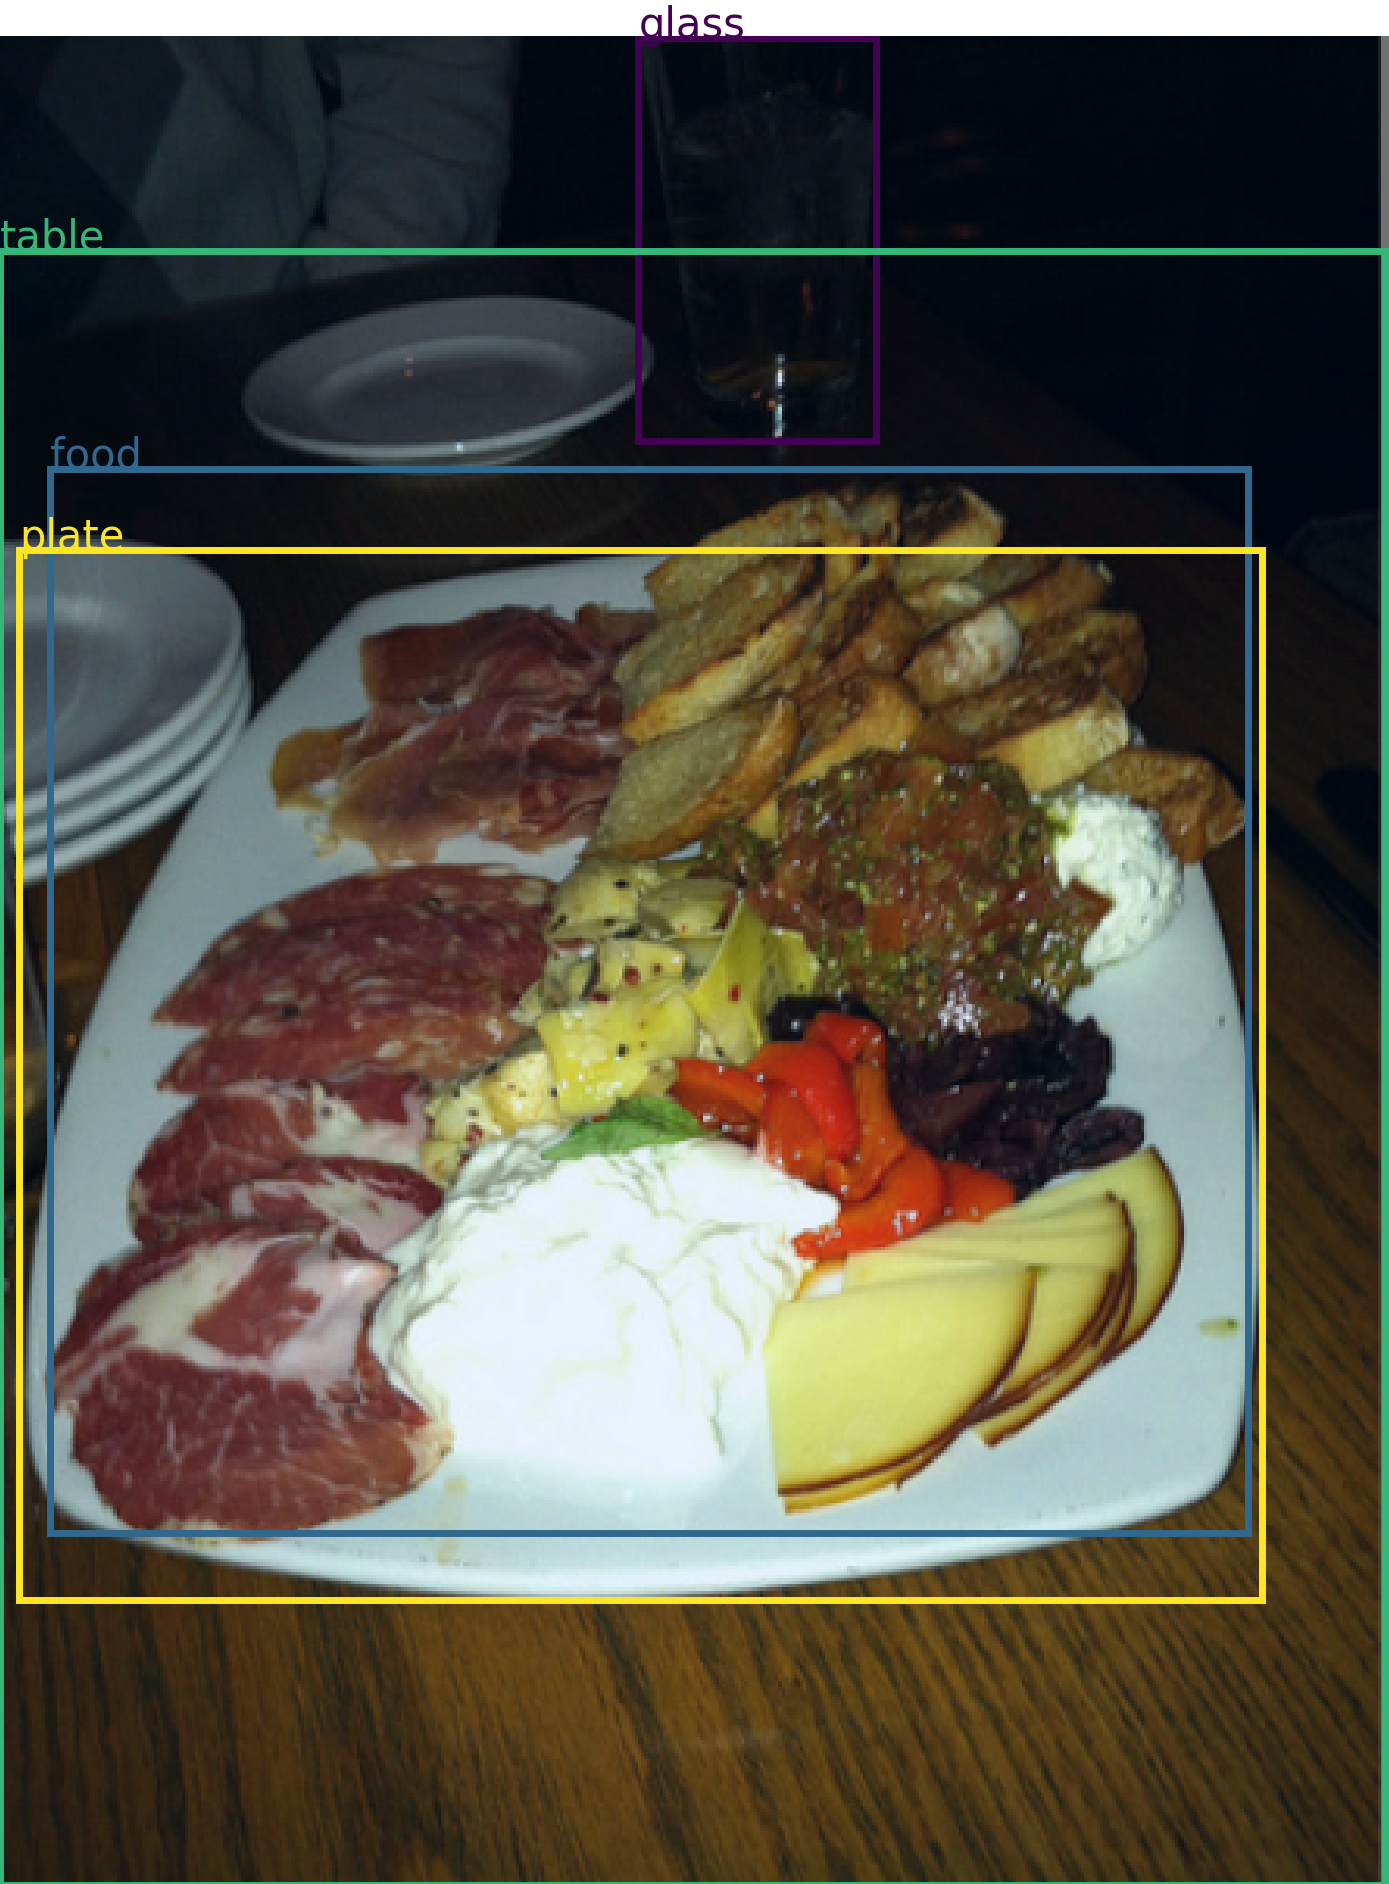
\includegraphics[width=0.9\linewidth]{figures/result/relation_Attention/img1}
		\end{minipage}
		\begin{minipage}[t]{6cm}
			\centering
			\includegraphics[width=0.86\linewidth]{figures/result/relation_Attention/img2}
	\end{minipage}}
	
	\subfigure[Grund truth realtion.]{
		\begin{minipage}[t]{6cm}
			\centering
			\includegraphics[width=1\linewidth]{figures/result/relation_Attention/rel1}
		\end{minipage}
		\begin{minipage}[t]{6cm}
			\centering
			\includegraphics[width=0.4\linewidth]{figures/result/relation_Attention/rel2}
	\end{minipage}}
	
	\subfigure[The attention between relations and objects in the Realtion Decoder.]{
		\begin{minipage}[t]{7cm}
			\centering
			\includegraphics[width=0.86\linewidth]{figures/result/relation_Attention/att1}
		\end{minipage}
		
		\begin{minipage}[t]{7cm}
			\centering
			\includegraphics[width=1\linewidth]{figures/result/relation_Attention/att2}
	\end{minipage}}
	
	\caption[The visualized results of the relation decoder attention.]{The visualized results of the relation decoder attention. We get the attention map from the second attention module of the relation decoder, it means which objects the relation pair pays more attention to, and the corresponding  attention weight will be higher in this map.}
	\label{fig:relation_attetnion}
\end{figure}


\begin{figure}[h!]
	\centering
	\subfigure[train]{
		\begin{minipage}[t]{5cm}
			\centering
			\includegraphics[width=0.9\linewidth]{figures/result/train/obj1}
	\end{minipage}}
	\subfigure[attention map with our loss]{
		\begin{minipage}[t]{5cm}
			\centering
			\includegraphics[width=0.9\linewidth]{figures/result/train/att1}
	\end{minipage}}
	\subfigure[ attention map without our loss]{
		\begin{minipage}[t]{5cm}
			\centering
			\includegraphics[width=0.9\linewidth]{figures/result/train/no1}
	\end{minipage}}
	
	\subfigure[haus]{
		\begin{minipage}[t]{5cm}
			\centering
			\includegraphics[width=0.9\linewidth]{figures/result/train/obj2}
			\label{fig:motor_man0}
	\end{minipage}}
	\subfigure[attention map with our loss]{
		\begin{minipage}[t]{5cm}
			\centering
			\includegraphics[width=0.9\linewidth]{figures/result/train/att2}
			\label{fig:motor_map0}
	\end{minipage}}
	\subfigure[attention map without our loss]{
		\begin{minipage}[t]{5cm}
			\centering
			\includegraphics[width=0.9\linewidth]{figures/result/train/no2}
			\label{fig:motor_man1}
	\end{minipage}}
	
	\subfigure[man]{
		\begin{minipage}[t]{5cm}
			\centering
			\includegraphics[width=0.9\linewidth]{figures/result/train/obj3}
			\label{fig:motor_man0}
	\end{minipage}}
	\subfigure[attention map with our loss]{
		\begin{minipage}[t]{5cm}
			\centering
			\includegraphics[width=0.9\linewidth]{figures/result/train/att3}
			\label{fig:motor_map0}
	\end{minipage}}
	\subfigure[attention map without our loss]{
		\begin{minipage}[t]{5cm}
			\centering
			\includegraphics[width=0.9\linewidth]{figures/result/train/no3}
			\label{fig:motor_man1}
	\end{minipage}}
	
	\subfigure[window]{
		\begin{minipage}[t]{5cm}
			\centering
			\includegraphics[width=0.9\linewidth]{figures/result/train/obj4}
			\label{fig:motor_man0}
	\end{minipage}}
	\subfigure[attention map with our  loss]{
		\begin{minipage}[t]{5cm}
			\centering
			\includegraphics[width=0.9\linewidth]{figures/result/train/att4}
			\label{fig:motor_map0}
	\end{minipage}}
	\subfigure[attention map without our loss]{
		\begin{minipage}[t]{5cm}
			\centering
			\includegraphics[width=0.9\linewidth]{figures/result/train/no4}
			\label{fig:motor_man1}
	\end{minipage}}
	
	\caption[The visualization of our attention loss of the first image in the test dataset]{The visualization of our attention loss of the first image in the test dataset.The first column is the object bounding box, the second column is the visualization result of the attention map when we use the attention loss, and the third column is the visualization result of the attention map without our attention loss.}
	\label{fig:train_attention_loss}
\end{figure}




\begin{figure}[h!]
	\centering
	\subfigure[bus]{
		\begin{minipage}[t]{5cm}
			\centering
			\includegraphics[width=0.9\linewidth]{figures/result/bus/obj1}
	\end{minipage}}
	\subfigure[attention map with our loss]{
		\begin{minipage}[t]{5cm}
			\centering
			\includegraphics[width=0.9\linewidth]{figures/result/bus/att1}
	\end{minipage}}
	\subfigure[attention map without our loss]{
		\begin{minipage}[t]{5cm}
			\centering
			\includegraphics[width=0.9\linewidth]{figures/result/bus/no1}
	\end{minipage}}
	
	\subfigure[man]{
		\begin{minipage}[t]{5cm}
			\centering
			\includegraphics[width=0.9\linewidth]{figures/result/bus/obj2}
	\end{minipage}}
	\subfigure[attention map with our loss]{
		\begin{minipage}[t]{5cm}
			\centering
			\includegraphics[width=0.9\linewidth]{figures/result/bus/att2}
	\end{minipage}}
	\subfigure[attention map without our loss]{
		\begin{minipage}[t]{5cm}
			\centering
			\includegraphics[width=0.9\linewidth]{figures/result/bus/no2}
	\end{minipage}}
	
	\subfigure[pants]{
		\begin{minipage}[t]{5cm}
			\centering
			\includegraphics[width=0.9\linewidth]{figures/result/bus/obj3}
	\end{minipage}}
	\subfigure[ attention map with our loss]{
		\begin{minipage}[t]{5cm}
			\centering
			\includegraphics[width=0.9\linewidth]{figures/result/bus/att3}
	\end{minipage}}
	\subfigure[ attention map without our loss]{
		\begin{minipage}[t]{5cm}
			\centering
			\includegraphics[width=0.9\linewidth]{figures/result/bus/no3}
	\end{minipage}}
	
	\subfigure[board]{
		\begin{minipage}[t]{5cm}
			\centering
			\includegraphics[width=0.9\linewidth]{figures/result/bus/obj4}
	\end{minipage}}
	\subfigure[ attention map with our loss]{
		\begin{minipage}[t]{5cm}
			\centering
			\includegraphics[width=0.9\linewidth]{figures/result/bus/att4}
	\end{minipage}}
	\subfigure[ attention map without our loss]{
		\begin{minipage}[t]{5cm}
			\centering
			\includegraphics[width=0.9\linewidth]{figures/result/bus/no4}
	\end{minipage}}
	
	\caption[The visualization of our attention loss of the second image in the test dataset]{The visualization of our attention loss of the second image in the test dataset.The first column is the object bounding box, the second column is the visualization result of the attention map when we use the attention loss, and the third column is the visualization result of the attention map without our attention loss.}
	\label{fig:bus}
\end{figure}



